\chapter{\color{oxfordblue} Machine Learning \& Deep Learning}\label{Chap-ML}
\ChapFrame

\textit{
This chapter is dedicated to a review of relevant machine learning and deep learning methods in the context of High Energy Physics (HEP). As for other fields of science and technology, the recent advancements in artificial intelligence have introduced many useful techniques that can be leveraged in particle physics. Before starting the review, a definition of the often confonded terminology is presented. This is followed by presenting the most commonly deployed approaches in particle physics: decision trees and deep neural networks. A final word on optimisation techniques is given at the conclusion of this chapter.
}

\section{Definitions}
\subsection{Artificial Intelligence}
Artificial Intelligence encapsulates any piece of software, any \textit{program}, that aims to mimic an aspect of human intelligence, a non-exhaustive list of which includes: 
\begin{itemize}
    \item \textit{Reasoning}, the ability to conduct logical thoughts and establish their validity.
    \item \textit{Inferring}, the ability to connect logical statements to induce or deduce new statements.
    \item \textit{Creating}, the ability to generate new content or information. 
    \item \textit{Acting}, the ability to perform a task or to modify the direct environment.
\end{itemize}
\gls{ai} research is a large field of investigation that studies these various aspects through numerous subjects such as robotics, \gls{nlp}, computer vision, generative modelling, and \gls{rl}. Artificial intelligence is broadly separated into three levels according to the performance of the underlying system: 
\begin{enumerate}
    \item \textit{Narrow Intelligence} represents artificial intelligence capabilities on a unique task, for which the software is specifically trained or designed. This field includes \textit{reactive \gls{ai}}, where a model is trained to output an optimal decision or prediction based on current conditions only and \textit{limited-memory \gls{ai}}, where a model can draw knowledge from past data to build an internal understanding of the problem to make better-informed decisions later. An example of the former is the IBM chess player Deep Blue, while the latter is most famously demonstrated by OpenAI's GPT model. 
    \item \textit{General Intelligence} refers to an artificial intelligence capable of matching human problem-solving skills in multiple environments. In particular, this hypothetical setting require machine to learn new tasks on their own and extrapolate from pre-acquired knowledge, a process referred to as \textit{transfer learning}. Such a model would have the ability to adopt and combine several of the traits of intelligence and to generalise the automated learning process to any task.
    \item \textit{Super Intelligence:} describes a hypothetical type of intelligence able to exceed human abilities and exhibit independent control of thoughts. 
\end{enumerate}

Of these, currently, only the first type is accessible and routinely deployed, with the second one the focus of ambitious research for state-of-the-art research laboratories. The inception of reactive \gls{ai}, the initial approach attempted, comes from the research into games in the 50s and 60s. This paradigm saw the rise of algorithms capable of searching for optimal moves in a large space of possible actions using \textit{heuristics}, human-passed knowledge on useful features of the specific environment of the game. For example, in chess one can use the point system assigning arbitrary values to each piece to help decide the worthiness of an action: e.g., a queen is typically worth more than a simple pion. In this reactive approach, neither the rules of the game nor the decision process are learnt. The former is forced into the search logic and the latter is the outcome of the search process. State space exploration of many realistic problems however scales asymptotically with the dimension of the input, quickly rendering reactive-based approaches impractical. Combined with the need for human-encoded insights into the problem, the potential of reactive \gls{ai} is restricted to specific well-controlled settings with a high degree of human understanding and low environment complexity. \\

limited-memory \gls{ai} revolutionised the field by removing the need for complete human control of the data interpretation and state formulation, letting instead a well-crafted mathematical model abstract and represent the information internally. It opens the door to applications that are not otherwise realistically tractable, such as autonomous driving, speech recognition, seamless robotics, etc. For such problems, complete programmatic problem formulations do not exist, prohibiting a reactive-based approach. The revolutionary paradigm of limited-memory \gls{ai} has been observed to outperform reactive \gls{ai} in all settings (e.g., in chess) and can be exploited in abstract scenarios where heuristics finding is impractical or intractable. For this reason, the focus of this chapter is on limited-memory \gls{ai} as exemplified by machine learning. 

\subsection{Machine Learning} 
Machine Learning (\gls{ml}) underpins the field of narrow \gls{ai} with limited-memory capabilities. It introduced a paradigm shift to the field, moving away from human-declared logic-based rules written in a specific syntax, the wholemark of reactive \gls{ai}. The lattter involves the execution of statements such as \[\textrm{\textit{If x happens, do y}},\] for an input $x$ and an output $y$. With limited-memory \gls{ai}, the state representation and decision steps are encoded in the mathematical models of the dataspace ($\mathcal{D}$) and the learning process: \[\forall\, x \in \mathcal{D}, \textrm{ do }f(x) = \hat{y}; \textrm{ update }f(x) \textrm{ given } (x, y),\] where $\hat{y}$ is the prediction of the model. In this case, both the internal representation of the rules and the decision-making are underpinned by the trained mathematical model $f$. Essentially, two distinct steps are applied to the model underpinned by adjustable parameters: 
\begin{enumerate}
    \item \textit{Inferring:} the model has to give its prediction $\hat{y}$ on a new data point $x$: $f(x) = \hat{y}$.
    \item \textit{Learning:} the parameters of the model are updated based on a specific training or fitting procedure, depending on whether the training will be progressively exposed to the data points of a training dataset or directly exposed to the entirety of the set. The objective is to align the output of the model $\hat{y}$ with the expected behaviour $y$: given the couple $(x, y)$, let $f(x) = \hat{y} \rightarrow y$ under training convergence. The model $f$ is trained to become an accurate estimator of the label $y$.
\end{enumerate}
The training process closely depends on the type of model being deployed. These can be broadly separated into two groups:
\begin{itemize}
    \item \textit{Classical machine learning:} covers models deploying specific algorithms to exploit the data in a pre-defined and fixed approach. They include linear regression, decision trees, Support Vector Machine (SVM), logistic regression, kernel methods, $k$-Nearest Neighbours, etc.
    \item \textit{\gls{dl}}: these methods are based on a core logical module called the \textit{artificial neuron}. This module is stacked into layers of given widths, meaning a given number of neurons, and several layers of such modules are then connected along depth. Within this category, the information flow through the network defines different types of \gls{dl}.
\end{itemize}
\gls{dl} is thus very much a part of \gls{ml}, constituting a specialised approach to building models from the core artificial neuron unit. Non-\gls{dl} are often referred to as \textit{classical} machine learning and still prove valuable in many applications thanks to their ease of use and their ability to be deployed in contexts with small dataset sizes. \gls{ml} can be deployed on various different tasks: 
\begin{itemize}
    \item \textit{Classification:} assigning a discrete variable called \textit{label}, to a datapoint: e.g., identifying $b$-jet. The general case is multiclass, with $n$ possible labels, and a particularly common case is binary classification ($n = 2$).
    \item \textit{Regression:} predicting a continuous variable for a datapoint: e.g., momentum reconstruction. 
    \item \textit{Features extraction:} given a dataset with specific internal features, construct new features, e.g., reconstructing the secondary vertex from a set of tracks. A special subcase of this category is embedding data points into a different hyperspace. The dimension of this final space can be larger, when embedding the data into a richer space, or smaller in the case of dimensionality reduction. A common example of the latter is \gls{pca}, which projects the data to a subspace spanned by the principal eigenvectors, those associated to the largest eigenvalues.
    \item \textit{Generation:} sampling new data from a distribution matching the training dataset distribution, e.g., sampling new $t\bar{t}$ events from a learnt statistical model. 
    \item \textit{Anomaly detection:} identify and flag rare events in an unlabelled dataset.
\end{itemize}

To perform these different tasks, models are constructed following different paradigms of \gls{ml}, divided according to the amount of human intervention \cite{MurphyML}:
\begin{itemize}
    \item \textit{Supervised learning:} the data used for training is endowed with the information the model must learn to predict. In the training step, the model is therefore optimised to make predictions that closely align with the target. Classification and regression are the most common tasks to fall under this realm.
    \item \textit{Unsupervised learning:} the data is not endowed with the extra information the model must predict but rather has underlying features that to be extracted. The model is therefore trained with an objective to optimise without explicit targets and should discover patterns and insights without guidance. Generative models and clustering are prime examples. 
    \item \textit{Semi-supervised learning:} also called \textit{weak supervision}, is a paradigm combining the supervised and unsupervised approaches. The model is mostly unsupervised but can benefit from some labelled cases or human input in \textit{active learning}. A prime example is to combine an unsupervised clustering task with a classification of the clusters. This is particularly fruitful when the cost of labelling the data is expensive, as is the case with real-world data.
    \item \textit{Self-supervised learning:} a machine instructs itself on what tasks to learn. The overarching goal of the model is loosely defined and the learning process includes superficial global objectives.
    \item \textit{Reinforcement Learning:} this paradigm of \gls{ml} is dedicated to the setting of a game-theoretic environment. An agent explores and interacts with an environment by choosing actions from a learnable policy by estimating its current situation and expected reward. In \gls{rl}, the agent learns to construct the best policy to satisfy a reward function and obtain the best outcome.
\end{itemize}
These different settings are particularly explored in deep learning, which is widely recognised as the most performant technique thanks to its ease of scaling in complexity.

\subsection{Deep Learning} 
\glsfirst{dl} refers to family of methods predominantly derived in the 1980s that have quickly grown in popularity in the last decade, with widely advertised results on competitive benchmark tasks in pattern recognition, such as the super-human performance of the \textit{DanNet} model \cite{DanNet} based on \glspl{cnn} \cite{NIPS198953c3bce6}. The basis of any deep learning method is the artificial neuron, a logical unit inspired by the design of a human neuron. Several such units are combined into layers of any number of neurons defining the width of the layer, and the layers are stacked into depth, with deeper layers receiving as input the output of earlier layers. Different \gls{dl} models are constructed by modifying the structure of the layers - in particular, the input, output, and activation function used - and the transfer of information between neurons, be that depth-wise between layers or width-wise between neurons. \gls{dl} is specifically well-suited to the setting of the ATLAS experiment, because:
\begin{itemize}
    \item Large datasets of both real and simulated data are available.
    \item Thanks to advanced \gls{mc} simulation programs of both the physics process and the detector reconstruction, the simulations are faithful representations of the real data.
    \item The data and data model from which the data originates is well understood in physics, the former coming from measurements from well-calibrated detectors and the second from crafted theories of the field. 
    \item The data exhibits rich features due to the collection of different detectors and the different scales of the underlying physics processes. The typical available representations span images, sequences, sets, and graphs, aligning with the main data representations studied by the deep learning community.
\end{itemize}
Given how important this form of \gls{ai} has become in all technological fields, this chapter is primarily dedicated to introducing some of its most relevant approaches for \gls{hep}. 

\section{Machine Learning Methods for Physics}
High-energy physicists enjoy a special relationship with machine learning. Experimental particle physics largely relies on statistical analyses of complex and large datasets, be that simulated using \gls{mc} methods or collected from sophisticated detector apparata. A typical \gls{hep} analysis can be described as five steps process:
\begin{enumerate}
    \item Data collection: real data is collected from a detector exposed to the underlying physics desired. 
    \item Simulated data is generated to match the condition of collection of the real data in terms of detector effects and operational conditions such as energy, \gls{pu}, and luminosity. This simulated data englobes the best of our current theoretical knowledge of the law of physics. 
    \item The detector required by modern particle physics experiment are composed of a complex set of subdetectors sensitive to different physical phenomena, as described in Chapter \ref{chapter-ATLAS}. The low-level information collected by different devices must be processed and recombined to generate \textit{objects}, aggregated information that hold physical meaning. This task corresponds to a mapping \textit{low}-level $\rightarrow$ \textit{high}-level information to reconstruct interesting and physically meaningful features of the measured data. 
    \item An analysis strategy is established, with the objective to similarly restrict the full datasets of both simulated and real data to a portion of the data that is most sensitive to the studied \textit{signal} or process. The sensitivity aspect underlies the need to take into account limitations in the knowledge of theoretical physics, the precision of the apparata, and the statistics of both simulated and measured events. To optimise the analysis, selection rules are derived based on physically accessible information, e.g., the centre-of-mass energy, the presence of leptons, the transverse momentum \pt, and other high-level objects reconstructed in the previous step.
    \item With the optimally selected set of real and simulated data points, a statistical model is built to quantify the agreement of the measured data with the expectations from the theory under the conditions of the experiment. This is often achieved through a profile likelihood computation, where the parameters of interest targeted by the analysis are measured to be those maximising the likelihood under the given measured data.
\end{enumerate}

Modern advanced machine learning has the potential to \textbf{improve all steps} of this process:
\begin{enumerate}
    \item The operational side of running the detector and the accelerators can benefit from \gls{rl} methods for improved control of the different electronic devices and online data quality monitoring. Triggers, an essential component of the ATLAS experiment described in Chapter~\ref{sub-sec-trigger}, can be upgraded to use sophisticated \gls{dl} models running online thanks to a hardware backbone built on \glspl{fpga} or \glspl{gpu}.
    \item Simulating a dataset through Monte Carlo is a computationally intensive task. Each event must pass through a selection of probabilistic steps, with only a simulated data point satisfying all requirements reaching the final sample. While This process can be optimised significantly with refined \gls{mc} methods, the cost remains significant to generate datasets of sufficient statistics. Generative \gls{ai} has the potential to accelerate this step by giving a statistical model that can be efficiently sampled. \gls{gan} and \gls{vae} have been shown to perform the sampling step in a competitive amount of time. However, a key current limitation of these approaches is the difficulty to fully incorporate the sophisticated theoretical model required to simulate the data, as any discrepancy or non-closure introduces levels of disagreements that are counter-productive in the final the physics analysis.
    \item \gls{ml} is particularly well-suited for object reconstruction. Broadly, machine learning offers scalable, efficient, and accurate techniques for this essential task. Important examples in ATLAS are particle identification (e.g., $\tau$ identification), \etm\ reconstruction, and heavy-flavour jets classification, as demonstrated in Chapter~\ref{chap-ftag}.
    \item Historically, physicists have relied on a cut-base approach to selecting data: the relevance of different variables is analysed for the physics problem at hand, to identify the best features to use to select events through manually defined restrictions. For example, in a leptonically decaying $Z$ boson measurement to two charged leptons $\ell^+\ell^-$, restricting the invariant mass of the lepton pair $m_{\ell^+\ell^-}$ to lie close the $Z$ boson rest mass is beneficial to select this process. Machine learning entirely bypasses this process, learning directly from an appropriate set of signal and background samples a transformation of the input features optimising the separation of signal from background. 
    \item The likelihood function of the constructed statistical test, quantifying the level of agreement between the real data and the theory through the simulated sample, can be directly learnt by a model given access to both sets. Additionally, anomaly detection, such as the search for unknown resonances, can be automated with unsupervised machine learning. 
\end{enumerate}

Contributing to step 3 in the aforementioned list is of the main focus of this thesis: developing \gls{dl}-tools for improved jet classification. The analysis presented in the latter part of the text also introduces some classical \gls{ml} techniques of data selection as suggested in step 4. 

\subsection{Decision Trees}
\glspl{dt}, also called \textit{Classification and Regression Trees} (CART), are the bread-and-butter of any data analysis. They are simple to train, give a good ground performance for both classification and regression, and are interpretable. The model relies on the recursive partitioning of the input space \cite{MurphyML}. Each partition step is a \textit{node} from which a tree structure emerges, where an initial \textit{root} state is subsequently partitioned along different branches with one \textit{leaf} per final output region. The splits are performed on the features of the input data, with the method accepting both discrete categorical values (e.g., the label of a lepton as $e, \mu, \tau$) and continuous values (e.g., $m_{\ell^+\ell^-}$). The following is a simple example of a classification tree outputting the predicted class as 0 or 1:

\Tree[.\textit{$x_i \leq c_i$} [.{True \\\textit{$x_j \geq c_j$}} [.True 1 ]
            [.False 0 ]]
        [.{False \\\textit{$x_k \leq c_k$}} [.True 0 ]
            [.{False \\{\textit{$x_l$} is \textit{$e$}}} [.True 0 ]
                            [.False 1 ]]]]

At each node, a condition is learnt with $x_i, x_j, x_k$ being continuous features of the dataset that are cut at the thresholds $c_i, c_j, c_k$ and $c_l$ is a categorical feature (e.g., is the lepton an electron). The leaves values are the output of the tree in different regions defined by the combination of successive selections - here a binary variable indicating a class. An example of a tree performing classification is shown in Figure~\ref{fig:tree-ex}, where a tree with two nodes can isolate most of the blue class from the red class with the region limited by green lines, corresponding to both conditions $x_1 \geq c_2$ and $x_2 \geq c_2$ being satisfied.

\begin{figure}[h!]
    \center
    \begin{minipage}[c]{0.3\textwidth}
        \caption{A binary classification problem with two features. A decision tree applies two successive cuts $c_1$ and $c_2$ to isolate most of the blue class from the red.}\label{fig:tree-ex}
      \end{minipage}
      \begin{minipage}[c]{0.5\textwidth}
        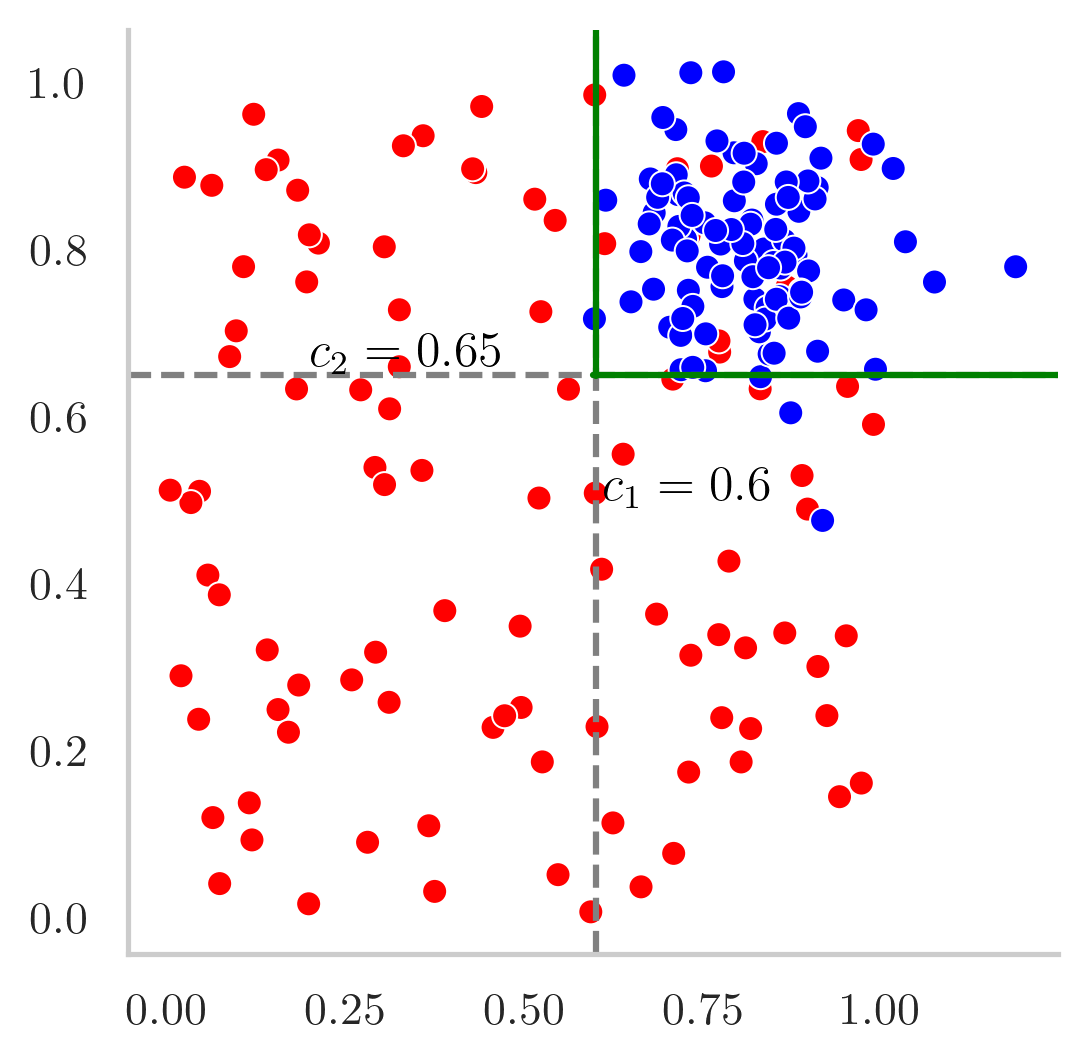
\includegraphics[width=\textwidth]{Images/ML/scatterPlot.png}
      \end{minipage}
\end{figure}
    
\paragraph{}Finding the optimal set of partitions of a dataset is an NP-complete problem and therefore intractable for large datasets. Instead, a greedy approach is adopted to build a tree, relying on a heuristic to find a satisfying solution. The most common approach is to successively choose the most optimal step at each stage with no guarantee to find a global optimum instead of a local one. The chosen split is selected based on a defined \textit{cost} function as
\begin{equation}\label{eq:DTcost}
    (j^*, t^*) = \arg\min_{j\in \{1, ..., D\},\, t \in T_j} \min \left(\text{cost} (\{x_i, y_i : x_{ij} \leq t\}) + \text{cost}(\{x_i, y_i : x_j > t\}) \right),
\end{equation}
where $T_j$ is the set of possible thresholds, and $x_j$ and $y_j$ are the features and labels (or regressive objectives). For categorical variables, the inequality $x_j >< t$ is converted into a value equality $x_j == t$. The \textit{cost} function depends on the objective of the tree, with the regression case typically using the \gls{mse} error function \[cost(D) = \sum_{i\in D}(y_i - \bar{y})^2,\] and for a classification the loss is often one of the following:
\begin{itemize}
    \item \textit{Missclassification rate:} $\frac{1}{|D|} \sum_{i \in D} \mathbb{I}(y_i \neq \hat{y})$, where $D$ is the data in the leaf of the tree and $\mathbb{I}$ is the identity operator defined as $\mathbb{I}(x) = 1$ if $x$ is True, else $0$. 
    \item \textit{Statistical entropy:} defining the class-condition probability as $\pi_c = \frac{1}{|D|} \sum_{i \in D} \mathbb{I}(y_i \neq c)$, the entropy over the $C$ classes is defined as
    \begin{equation}\label{eq:statEntropy}
        H(\boldsymbol{\pi}) = - \sum_{c=1}^C \pi_c \log \pi_c,
    \end{equation}
    with $boldsymbol{\pi}$ a vector ($\pi_1, \pi_2, ..., \pi_C$) of the class-condition probabilities.
    \item \textit{Information Gain:} an equivalent formulation to the entropy, measuring the gain in information from the change in entropy induced by adding a selection on feature $X_j$ to the current selection 
    \[ \text{Gain}(X_j < t, Y) = H(Y) - H(Y | X_j < t) \]
    \item \textbf{Gini:} computes and minimises the expected error rate:
    \begin{equation}\label{eq:giniClass} 
        \sum_{c=1}^C \pi_c (1 - \pi_c).
    \end{equation}
\end{itemize}

The pseudocode algorithm to train a \gls{dt} with the update rule of Equation \ref{eq:DTcost} is summarised in Algorithm \ref{ag:DT}. 

\begin{algorithm}
    \caption{Recursive Procedure to Train a Decision Tree \cite{MurphyML}.}
    \begin{algorithmic}
    \Function{fitTree}{node, $D$, depth}
        \State $\text{node.prediction} \gets \text{mean}(\{y_i : i \in $D$\})$ 
        \State $(j^*, t^*, D_L, D_R) \gets \text{split}(D)$
        \If{\text{not worthSplitting}(\text{depth}, \text{cost}, $D_L$, $D_R$)}
            \State \Return node
        \Else
            \State node.left $\gets$ \textsc{FitTree}(node, $D_L$, depth + 1)
            \State node.right $\gets$ \textsc{FitTree}(node, $D_R$, depth + 1)
            \State \Return node
        \EndIf
    \EndFunction
    \end{algorithmic}
    \label{ag:DT}
\end{algorithm}

\glspl{dt} can overfit a dataset, when the model tunes itself to specific features of the training set that do not generalise. Regularisation serves as an important step to contain this mostly undesirable behaviour. For trees, a common procedure to avoid overtraining is to interrupt the growth of the tree when it is no longer worth doing so or to \textit{prune} the tree by removing nodes or branches that contribute little to the overall performance. A simpler way to regularise the performance by reducing the variance of the estimate of the model is to train several trees with different random subsets of the data and aggregate the results into a single prediction. For example, taking as regressive output the average over several $N_l$ base learners \[ y(x) = \frac{1}{N_l} \sum_{i=1}^{N_l} y_i(x),\] over base learner predictions $y_i(x)$ for a common input $x$. For classification, the predicted class can be decided with majority voting. This statistical technique of combining different predictors is referred to as \textit{bagging} or \textit{ensembling}. The different predictors can be built on subsets of the input features and training datapoints to further decorrelate them, thereby forming a \textit{random forest}.

\subsection{Boosted Decision Trees}
A popular extension to the simple \gls{dt} approach is to introduce the concept of \textit{boosting}, leading to a technique referred to as \textit{\glsfirst{bdt}} or \textit{\glsfirst{mva}}. Boosting is a greedy algorithm leveraging a weak learner and applying it sequentially to weighted versions of the data, with a larger weight given to misclassified datapoints. This method is hugely popular in data science, having earned the title \textit{``best off-the-shelf classifier in the world''} \cite{baggingML}. Two particularly useful approaches are adaptive boosting (AdaBoost) \cite{Adaboost} and gradient boosting \cite{gradientBoosting}, both combining an ensemble of $M$ weak learners $f_i$ ($i = 1, ..., M$) into a strong learner $F$: \[F(x) = \sum_{i=1}^M f_i(x).\] For the following discussion, the model is built using a training dataset $ \{(x_1, y_1), ..., (x_N, y_N)\}$ with input vectors $x_i \in \{\mathbb{R} \otimes \mathbb{D}\}^d$ of $d$ features that are real or discrete ($\mathbb{D}$) and $y_i \in \mathbb{R}^d$ is a $d$-dimension real vector that serves as output to be predicted by the model.

\subsubsection{AdaBoost}\label{sub-adaboosted}
AdaBoost combines the $M$ weak learners $f_i$ with adaptive weights $\alpha_i$ to improve the ensemble performance as \[F(x) = \sum_{i=1}^M \alpha_i f_i(x),\] where $F$ is the boosted model, and the successive boosting stages $F_T = \sum_{i=1}^{T \leq M} \alpha_i f_i(x)$ define stronger combinations of the weak learners $f_i$ with weights $\alpha_i \in \mathbb{R}$. At each iteration $m$ of the training process ($m = 1, ..., M$), a weak learner $f_m$ is fitted to the training set to minimise a loss function $L(y_i, F_{m}(x_i))$. AdaBoost relies on the exponential loss
\begin{equation}\label{eq:adaboosterror}
    L(y, F_m(x)) = \sum_{i=1}^N \exp\left(-y_i F_m(x_i)\right) = \sum_{i=1}^N \exp\left(-y_i (F_{m-1}(x_i) + \alpha_m f_m(x_i))\right),
\end{equation}
that the new weak learner $\alpha_m f_m$ added at step $m$ has to minimise. The typical case for AdaBoost is binary classification with $y_i \in \{-1, 1\}$, but the algorithm is generalisable to multi-class \cite{MurphyML}. Equation \ref{eq:adaboosterror} can be re-expressed as: \[\sum_{i=1}^N w_{i,m} \exp\left(-\alpha_m y_i f_m(x_i)\right),\] where $w_{i,m} = \exp\left(-y_i F_{m-1}(x_i)\right)$ is interpreted as a weight applied to the datapoint $(x_i, y_i)$  indexed by $i$ at step $m$ proportionaly to the error of the current strong learner. One can show that the weak learner $f_m$ minimising the optimisation objective at step $m$ is the one minimising the miss-classified weights sum error $\epsilon_m$ of the reweighted version of the dataset with weights $w_{i,m}$ \cite{MurphyML}, where \[\epsilon_m = \sum_i w_{i,m} \mathbb{I}(y_i \neq f_m(x_i)).\] For the first step $m = 1$, the weights are initialised to $1 / N$. They are then updated to \[w_{i,m+1} = w_{i,m} e^{-\alpha_m y_i f_m(x_i)},\] and renormalised so that $\sum_i w_{i, m+1} = 1$ before being assigned to each training input in the next step. The weak learner is combined with the strong learner using an optimal weight $\alpha_m$ found by minimising the loss $L$ of the combined learner \[\alpha_m = \frac{1}{2} \log \frac{1 - \epsilon_m}{\epsilon_m},\] giving the overall update rule
\begin{equation}\label{eq:updateOverall}
    F_m(x) = F_{m-1}(x) + \alpha_m f_m(x),
\end{equation}
that combines the new weak learners $f_m$ with optimal weight $\alpha_m$ to the current strong learner $F_{m-1}$. The AdaBoost algorithm is summarised in Algorithm \ref{algo:adaboost}.

\begin{algorithm}
    \caption{Adaboost for Binary Classification with Exponential Loss \cite{MurphyML}}
    \label{algo:adaboost}
    \begin{algorithmic}
    \State Initialise weights: $w_{i,1} = 1/N$, where $N$ is the number of samples.
    \For{$m = 1$ to $M$}
        \State Minimise $\epsilon_m = \sum_i w_{i,m} \mathbb{I}(y_i \neq f_m(x_i))$ on training set with weights $w_{i,m}$ to find $f_m(x)$.
        \State Compute $\alpha_m = \frac{1}{2} \log\left(\frac{1 - \epsilon_m}{\epsilon_m}\right)$.
        \State Update weights: $w_{i,m+1} \leftarrow w_{i,m} \, \exp(-\alpha_m y_i f_m(x_i))$ and renormalise $\sum_i w_{i, m+1} = 1$.
    \EndFor
    \State \Return $F(x) = \sum_{m=1}^M \alpha_m f_m(x)$
    \end{algorithmic}
\end{algorithm}

\subsubsection{Gradient boosting}\label{sec-gradient-boost}
Gradient boosting is a generic approach which, contrary to AdaBoost, is not restricted to a specific loss function. The objective to minimise is the empirical risk, the expected value of the loss function $L$ on the training set 
\begin{equation}\label{eq:empRisk}
    \hat{f}  = \arg \min_f \mathbb{E}_{x,y} L(y, f(x)).
\end{equation}
As the name suggests, the approach leverages gradient descent to find the optimal $\hat{f}$. At step $m$, the gradient of the loss $L$ is evaluated at $f = f_{m-1}$ as \[ g_{i,m} = \left[ \frac{\partial  L(y_i, f(x_i))}{\partial f(x_i)} \right]_{f= f_{m-1}}, \] which is then used to update the learner with a step $f_m = f_{m-1} - \alpha_m g_{m},$, where $g_m$ is the gradient of each datapoint and the step-length $\alpha_m$ is chosen to minimise the residual loss $L(y, f_{m-1}$ $- \alpha_m g_{m})$. This implements functional gradient descent and leads the model to fit the $N$ datapoints of the set. This procedure naturally leads to overfitting, an undesirable feature that is remedied by using a weak learner to approximate the negative gradients. In the specific case of gradient-boosted decision trees, at step $m$ a decision tree $h_m(x)$ is fitted to the pseudo-residuals $g_{i,m}$. This \gls{dt} $h_m$ at step $m$ defines $J_m$ disjoint regions through its leaves with predictions $b_{jm}$ in each region indxed by $j = 1, ..., J_m$: \[ h_m(x) = \sum_{j=1}^{J_m} b_{jm} \textbf{1}_{R_{jm}}(x),\] where $\textbf{1}_{R_{jm}}(x)$ is the indicator function - equals to 1 when $x \in R_{jm}$ and 0 otherwise. The model update is \[f_m(x) = f_{m-1} + \alpha_m h_m(x),\] with $\alpha_m$ selected by minimising the empirical risk \[ \alpha_m = \arg \min_{\alpha} \sum_{i=1}^N L\left(y_i, f_{m-1}(x_i) + \alpha h_m(x_i)\right).\]

The full algorithm for gradient boosting is presented in Algorithm \ref{algo:gradient_boosting}, where the update rule is added a \textit{learning rate} hyperparameter $lr$ to introduce regularisation and reduce the risk of overfitting. By keeping $0 < lr \leq 1$, the ability of the model to fully adapt to the training error is limited, thereby improving generalisation to unseen data. The price is a slower updating of the model and a higher computational complexity. Further regularisation techniques are bootstrap aggregation - training each weak learner on a random subset of the data -, limiting the number of leaves, penalising models of larger complexity, and pruning branches that do not sufficiently reduce the loss. \\

\begin{algorithm}
    \caption{Gradient Boosting \cite{MurphyML}}
    \label{algo:gradient_boosting}
    \begin{algorithmic}
    \State Initialise $f_0(x) = \arg\min_\alpha \,\sum_{i=1}^N L(y_i, \alpha)$
    \For{$m = 1$ to $M$}
        \State Compute the gradient residuals for each $i= 1, ..., N$: $g_{i,m} = -\left[\frac{\partial L(y_i, f(x_i))}{\partial f(x_i)}\right]_{f(x_i) = f_{m-1}(x_i)}$
        \State Train weak learner $h_m$ on the dataset $\{(x_i, g_{i,m})\}_{i=1}^N$
        \State Compute $\alpha_m$ by minimising $\sum_{i=1}^N L(y_i, f_{m-1}(x_i) + \alpha h_m(x_i))$
        \State Update $f_m(x) = f_{m-1}(x) + lr \times \alpha_m h_m(x)$
    \EndFor
    \State \Return $f(x) = f_M(x)$
    \end{algorithmic}
\end{algorithm}

\glspl{bdt} resist better to overtraining thanks to the regularisation effect. An undesirable feature of boosting is the loss of direct interpretability of the decision-making. This is however more than met by an appreciable gain in performance of the underlying model. An interesting property exhibited by all tree-based algorithms and many \gls{ml} approaches is the ease of quantifying the impact of a specific feature on the result. This technique of \textit{feature importance} assigns a score to each input feature, typically the Gini importance of Equation \ref{eq:giniClass}. Another popular technique taken from the field of cooperative game theory is the Shapley value, measuring the average marginal contribution of each feature to the objective function \cite{shapley:book1952, Rozemberczki2022TheSV}.

\paragraph{Pros:}
\begin{itemize}
    \item \textit{High Accuracy:} \glspl{bdt} easily achieve high accuracy in many tasks.
    \item \textit{Ease of Deployment:} \glspl{bdt} typically perform reasonably well out-of-the-box and are easy to train with few hyperparameters to optimise. 
    \item \textit{Adaptability to Different Distributions:} boosting algorithms adapt to different types of data distributions and capture non-linear relationships.
    \item \textit{Ensemble Learning:} combining multiple weak learners to create a strong learner improves the overall model performance. 
    \item \textit{Robustness to Overfitting:} boosting mitigates overfitting, enhancing the generalisation of the model to unseen data. 
\end{itemize}

\paragraph{Cons:}
\begin{itemize}
    \item \textit{Sensitivity to Noisy Data:} \glspl{bdt} are sensitive to noisy data and outliers.
    \item \textit{Computational Complexity:} Training multiple weak learners sequentially can be computationally expensive, especially on large datasets.
    \item \textit{Parameter Tuning:} \glspl{bdt} require some fine-tuning of the hyperparameters for optimal performance.
    \item \textit{Black Box Nature:} The ensemble nature of \glspl{bdt} make them somewhat of a black box, sacrificing the interpretability of \glspl{dt} for the sake of performance.
\end{itemize}

\subsection{Artificial Neurons}
The Artificial Neuron or \textit{perceptron}, as initially named by its inventor Frank Rosenblatt in his seminal 1958 paper \cite{rosenblatt1958perceptron}, is the logical unit at the core of modern deep learning. Notably, the \gls{mlp} or \gls{dnn} are obtained by stacking layers of artificial neurons. Inspired by biological principles, the perceptron, shown in Figure~\ref{fig:annModel}, accepts multiple inputs and gives as output 1 if the combination of inputs exceeds a certain modifiable threshold, otherwise giving 0. This combination accepts weights to scale the input which are modified during training to correct the output of the perceptron. Artificial neurons are a direct generalisation on this principle, with the output no longer being thresholded but applied a chosen function $f$ after being added a learnable bias term $b$. 

\begin{figure}[h!]
    \center
    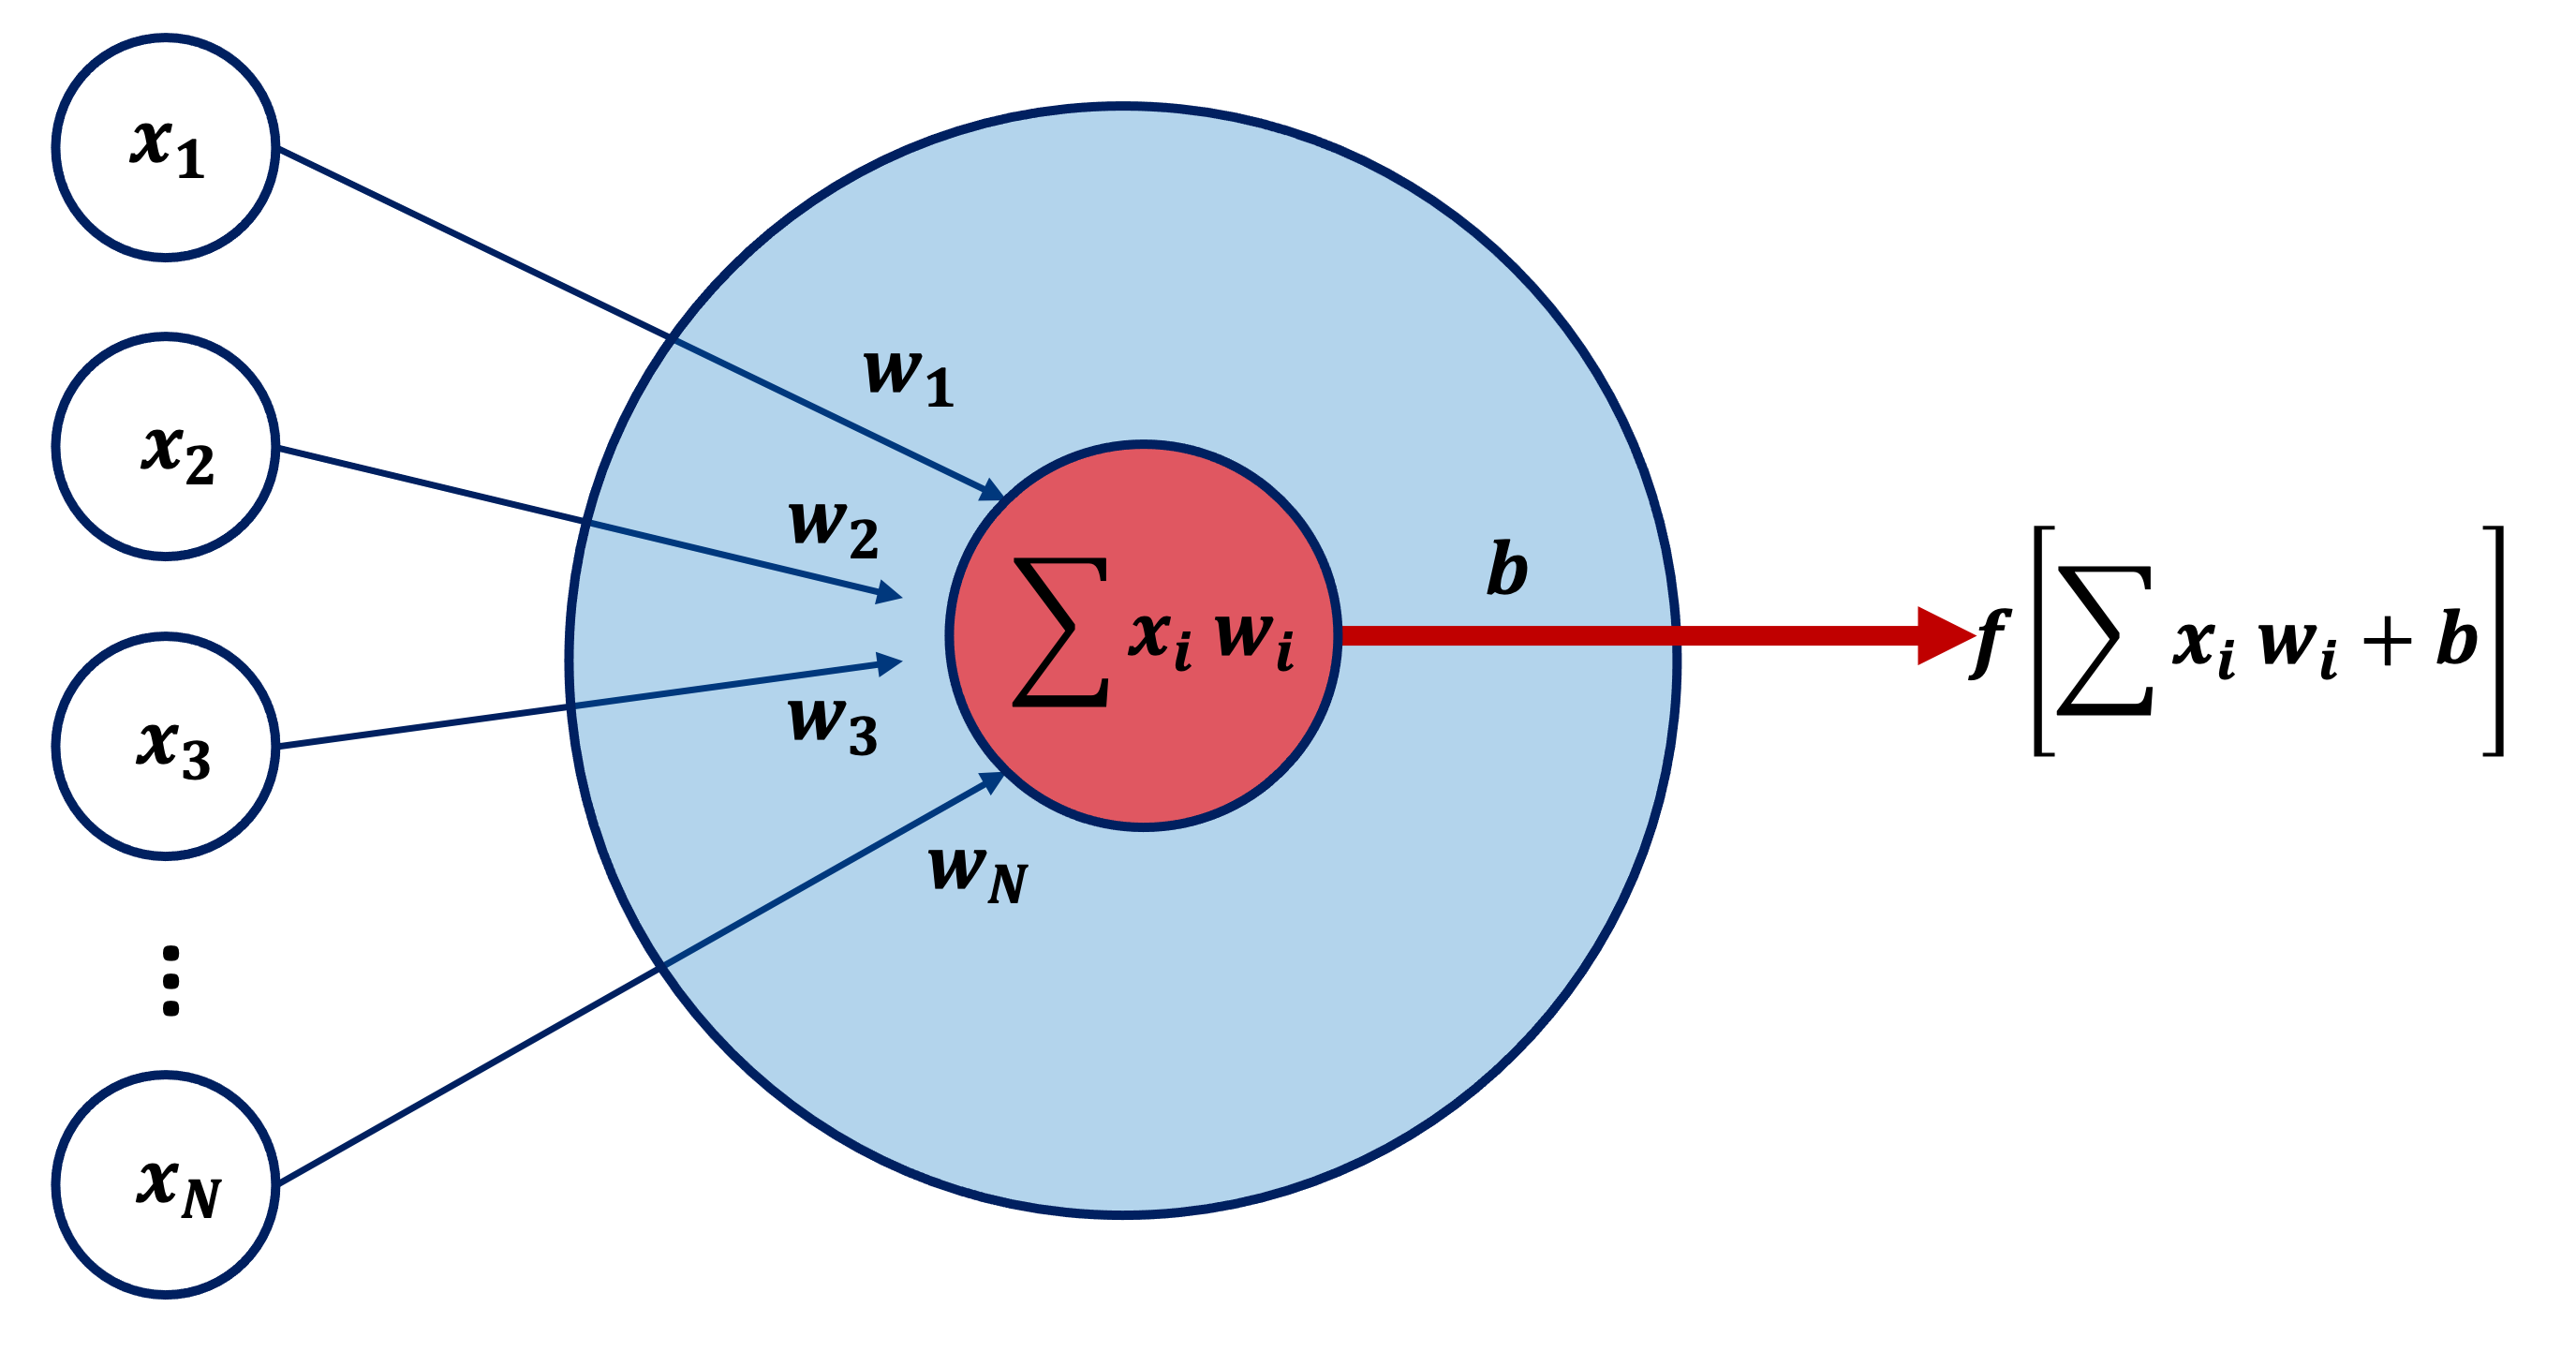
\includegraphics[width=0.8\textwidth]{Images/ML/ann.png}
    \caption{An artificial neuron: the inputs $x_i$ ($i= 1, ..., N$) are multiplied by learnable weights $w_i$, summed and added a learnable bias $b$ and passed to an activation function $f$.} 
    \label{fig:annModel}
\end{figure}

\paragraph{} The interest in artificial neurons stems from a significant theoretical result: stacks of artificial neurons are \textit{universal function approximator} \cite{universalFuncApproxNN,HORNIK1989359}, as shown in the next section. This theoretical result is built on a mathematically advantageous function chosen for $f$: the sigmoid $\sigma$, defined in equation \ref{eq:sigmoid} and shown in Figure~\ref{fig:sigmoid}:
\begin{wrapfigure}{r}{0.5\textwidth}
    \begin{center}
        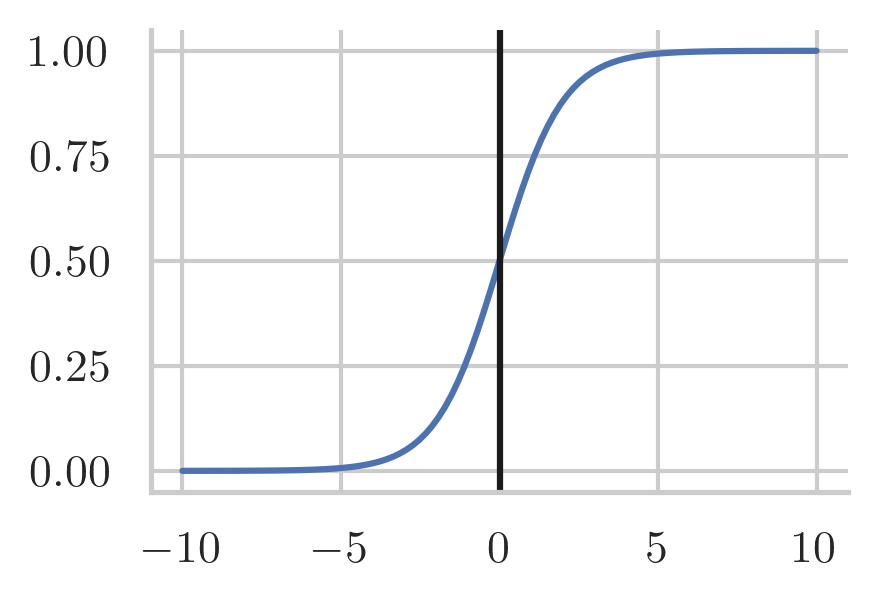
\includegraphics[width=0.4\textwidth]{Images/ML/sigmoid.png}
        \caption{The sigmoid function $\sigma$.} 
        \label{fig:sigmoid}
    \end{center}
\end{wrapfigure}

\begin{equation}\label{eq:sigmoid}
    \sigma(x) = \frac{1}{1 + e^{-x}}.
\end{equation}

Thanks to its property to map the set of real numbers to the [0, 1] range, this activation function is often used for numerical stability and probability distribution mappings. An essential mathematical property of the sigmoid, particularly relevant for \gls{dl}, is the ease to compute its derivative: \[\sigma^\prime(x) = \sigma(x) (1- \sigma(x)).\]

The power of artificial neurons stems from the ability to be efficiently combined them into ordered structure with powerful representation powers. For an input $x \in \mathbb{R}^d$, a neuron individually applies an affine transformation $W_i^T x + b_i$, where $W_i \in \mathbb{R}^d,\,b_i \in \mathbb{R}$ are the weights and bias of the neuron $i$, that is passed through an activation function $f$ for a total output of a single neuron $f(W_i^T x + b_i)$. Combining these operations leads to a mathematical model that can approximate any continuous function. 

\subsection{Deep Neural Networks}
A Deep Neural Network (\gls{dnn}) - also called Multilayer Perceptron (\gls{mlp}), \gls{ann}, feed-forward neural network, or sometimes only \gls{nn} - is constructed by stacking layers of artificial neurons as shown in Figure~\ref{fig:neuralnet}. Each neuron in a layer receives as input the output of the neurons of the previous layer, and connects to the neurons of the next layer. Layers of artificial neurons that are placed between the input and output ones are said to be \textit{hidden layers}. The particularity of the design underpinning this architecture is that layers of neurons connect to all neurons of the next layers only, defining a feed-forward computation graph flowing from the input $x$ to the output $y$. Mathematically, a single layers at depth $i$ with $m$ units given as input the previous $n$-neurons layer at depth $i-1$ computes an affine transformation
\begin{equation}\label{eq:feedforward}
    a^i = f^i\left({W_i}^T a^{i-1} + b_i\right),
\end{equation}
where $W^i \in \mathbb{R}^{m \times n}$ is the matrix of learnable weight of layer $i$ - one row per unit of layer $i$, one column per unit of layer $i-1$, $b_i \in \mathbb{R}^m$ the vector of learnable biases, $f^i$ is the activation function of layer $i$, and $a^{i-1} \in \mathbb{R}^n$ are the $n$ activated outputs of the previous layer. The activations can differ for the units of the same layer but are often kept similar to vectorise the mathematical operations. 

\begin{figure}[h!]
    \center
    \begin{minipage}[l]{0.38\textwidth}
        \caption{A deep neural network with $d$ layers of width $m$, $l$ ..., $k$. Each artificial neuron, represented by a ball of darkening blue along the depth, computes an affine transformation of the input of the layer followed by an activation function. The input of the \gls{dnn} is $x$ and the output is $y$.} 
    \label{fig:neuralnet}
      \end{minipage}
      \begin{minipage}[c]{0.6\textwidth}
        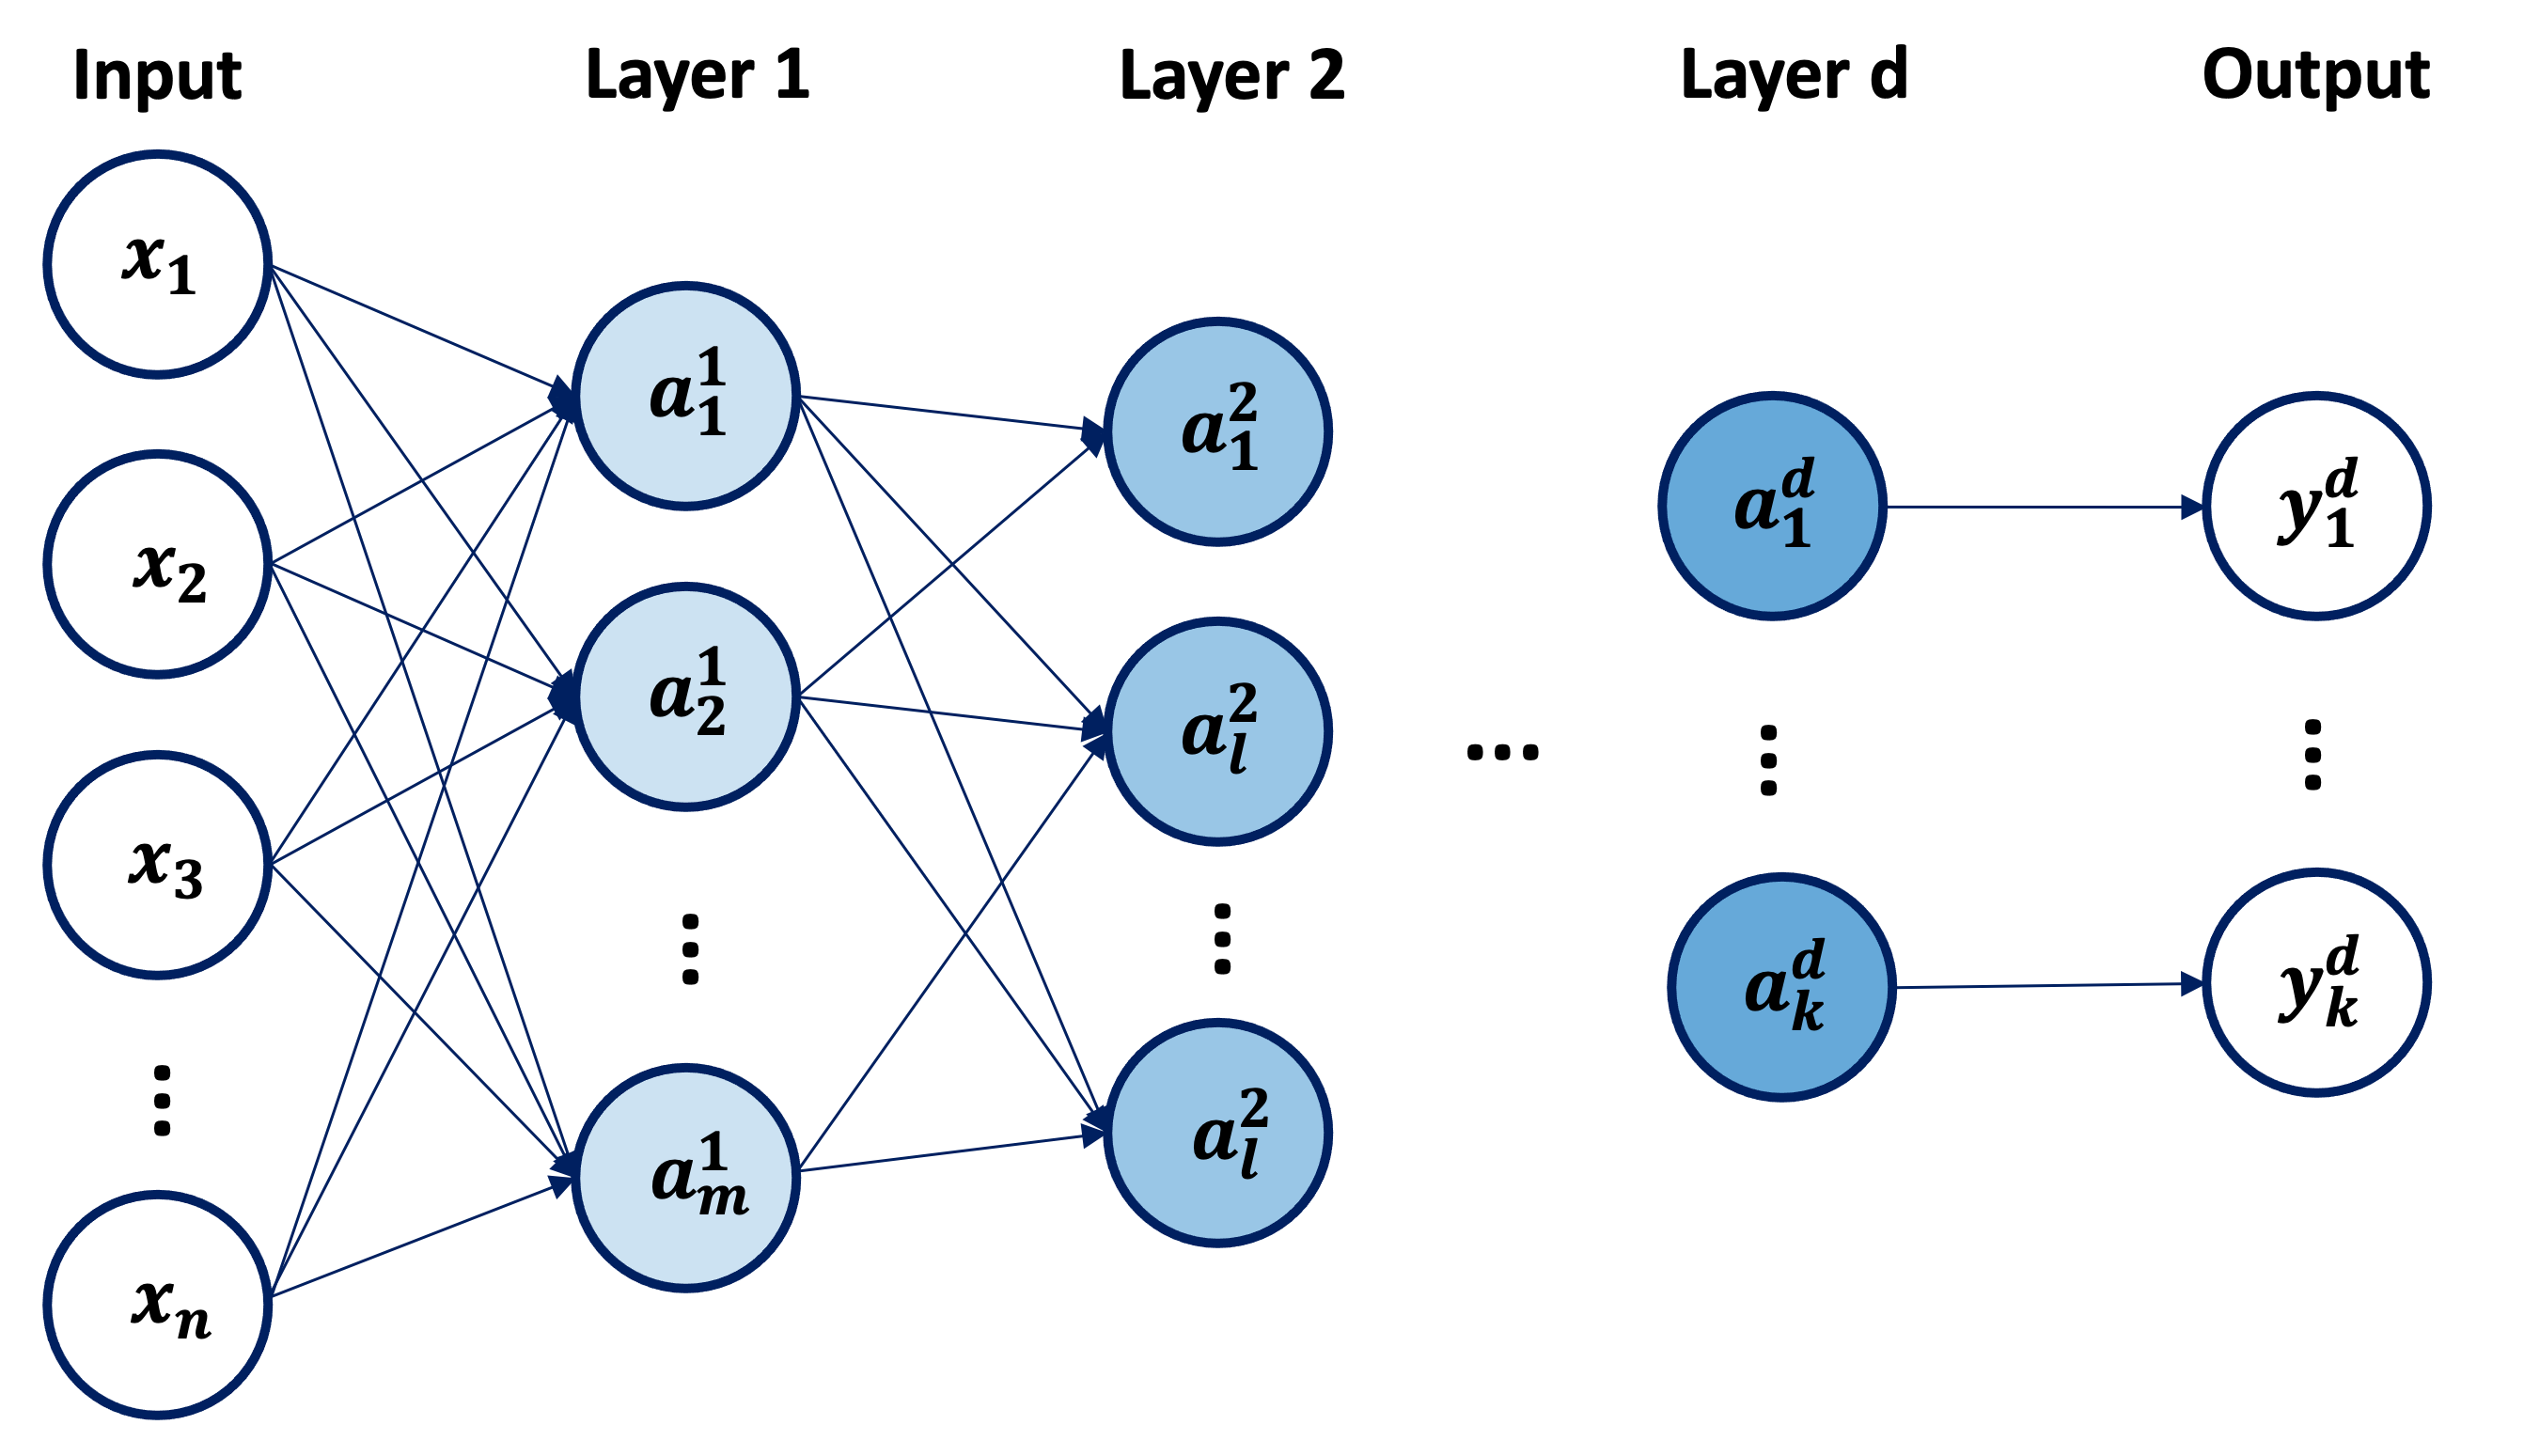
\includegraphics[width=\textwidth]{Images/ML/neuralnet.png}
      \end{minipage}
\end{figure}

\paragraph{}Neural networks implement a recursive system of computation based on Equation~\ref{eq:feedforward}. A powerful theoretical property of neural networks is their capacity to be \textit{Universal Function Approximators}. This family of theorems, defined for various types of activations and network, demonstrates that neural networks built with appropriate activation functions and sufficient capacity are able to approximate most well-behaving functions. The most famous such theorem states \cite{universalFuncApproxNN,HORNIK1989359}:

\paragraph{Theorem:} \textit{Let $C([0, 1]^n)$ denote the set of all continuous functions $[0, 1]^n \rightarrow \mathbb{R}$ and $\sigma$ be any sigmoidal activation function. Then the finite sum $\hat{f}(x) = \sum_{i=1}^N \alpha_i \sigma(w_i^T x + b_i)$ is dense in $C([0, 1]^n)$. In other words, given any $f \in C([0, 1]^n)$ and $\epsilon > 0$, there is a sum $\hat{f}(x)$ of the above form for which \[ f(x) - \hat{f}(x)| < \epsilon \quad \forall x \in [0, 1]^n.\]}

The theorem essentially establishes that any function defined over the $n$-dimensional unit hypercube $[0, 1]^n$ can be approximated by an arbitrarily wide neural network. This result only requires $\sigma$ to be sigmoidal or discriminatory in the sense
\begin{equation}
    \sigma(x) \rightarrow
    \begin{cases}
        1 \text{ if } x \rightarrow \infty,  \\
        0 \text{ if } x \rightarrow -\infty,
    \end{cases}
\end{equation}
which is satisfied by the sigmoid function. This result can be applied outside the unit hypercube by a homothetic transformation of the data space. Many flavours of \gls{dnn} exist with different functions used. An important theoretical result is the requirement for the output function applied to the artificial neuron to possess some degree of \textit{non-linearity}. A neural network with strictly linear functions would indeed collapse into a linear regression model. Such a non-linear function, when applied to the output of an artificial neuron, is said to \textit{activate} it and is hence called \textit{activation functions}. Interestingly, similar theorems were derived for the most important activation functions commonly used in deep learning \cite{universApproximator-Relu}. Som e common activation functions, shown in Figure~\ref{fig:commonAct}, are:
\begin{itemize}
    \item The sigmoid function of Equation \ref{eq:sigmoid}.
    \item The hyperbolic tangent function tanh$(x) = \frac{e^x - e^{-x}}{e^x + e^{-x}}$.
    \item The \gls{relu} function\cite{agarap2019deep}
    \begin{equation}\label{eq:relu}
        \text{ReLu}(x) = \text{max}(0, x).
    \end{equation}
    The non-linearity here is strictly between positive and negative inputs, making this activation function the simplest that can be leveraged in \gls{dnn}. A generalisation of \gls{relu} called leakyReLU $= \max(\alpha x, x)$ introduces a linear function in the negative range, with $\alpha \in [0, 1[$. 
    \item The Exponential Linear Unit (ELU) function modifies the leakyReLU in the negative domain while keeping the saturation property as
    \begin{equation}\label{eq:elu}
        \text{Elu}(x) = 
        \begin{cases}
            x \quad \text{ if } x >= 0, \\
            \alpha (e^x - 1) \text{ otherwise},
        \end{cases}
    \end{equation}
    with the hyperparameter $\alpha > 0$.
    \item The softmax function which, for an $x \in \mathbb{R}^n$, return a vector softmax$(x) = [..., \frac{e^{x_i}}{Z}, ...]$ with $Z = \sum_i e^{x_i}$. For a 2-dimensional $x$, the softmax is equivalent to the sigmoid. In $n$-dimension, it maps each entry of $x$ to the range $[0, 1]$ and guarantees $\sum_i $softmax$(x)_i = 1$. The softmax is therefore helpful to define probability distributions over multidimensional outputs.
\end{itemize}

\begin{wrapfigure}{R}{0.5\textwidth}
    \begin{center}
        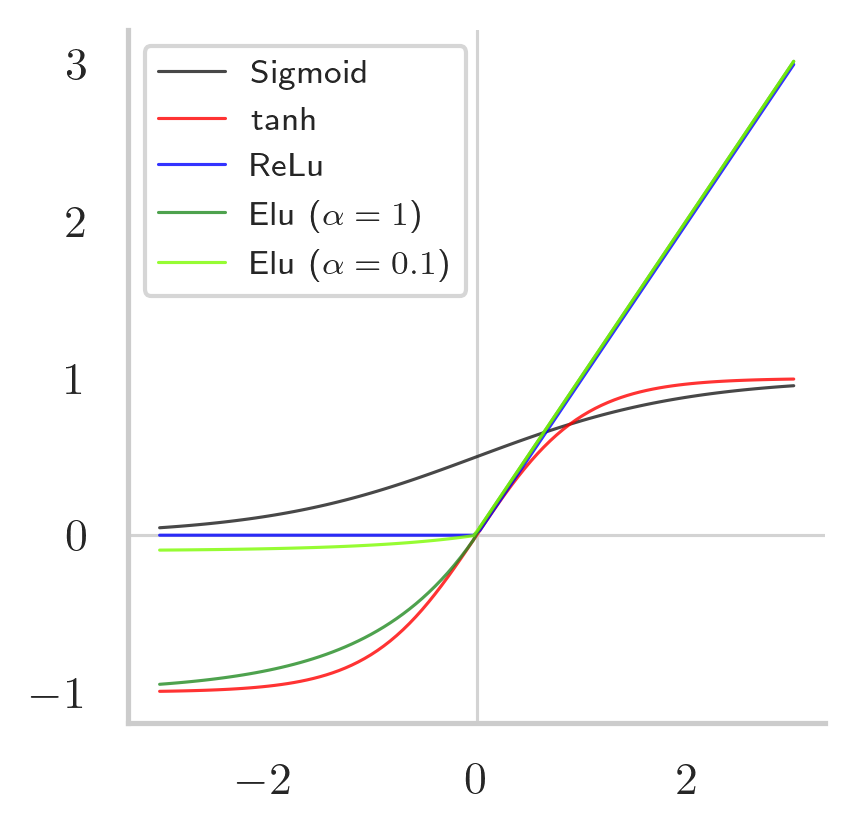
\includegraphics[width=0.45\textwidth]{Images/ML/activations.png}
        \caption{The most common non-linear activations used in deep learning.} 
        \label{fig:commonAct}
    \end{center}
\end{wrapfigure}

The sigmoid is no longer the choice of reference, due to its tendency to quickly saturate - meaning its gradient for large positive or negative values \textit{vanishes} by tending to 0. The hyperbolic tangent offers larger gradients thanks to its [-1, 1] range with steeper curvature, making it the activation of choice for autoregressive architecture such as the \gls{rnn}. The \gls{relu} function is the most widely used activation function as its derivative is trivial and does not suffer from vanishing gradients for positive values. Its fixed 0-value for negative input is a double edge sword: on one side, it helps the network regularise itself by deactivating neurons, on the other some neurons can be stuck in \textit{off}-mode. For this reason, it is important to correctly initialise the weights of a \gls{dnn}. A workaround for this limitation is the introduction of leakage for the negative inputs with leakyReLU or Elu activations.\\

While the Universal Function Approximator theorem is a powerful endorsement of neural netowrks, it does not state \textit{how} to derive the best network. The task of choosing the right architecture depthwise and widthwise and the correct weights and biases is approximated by a learning strategy updating the parameters to reduce the error between the empirical risk. What sets apart neural networks from other Universal Function Approximators is the simplicity of the procedure to update their weights: with a suitable computational structure and activation function choice, the \glspl{nn} are \textit{differentiable}. Gradients can therefore be computed from a loss function measuring the quality of the output $\hat{y}$ and \textit{backpropagated} across the neurons to update the weights and biases. The recent rise of \gls{dl} in \gls{ai} can be traced back to improvements in making this backpropagation of the gradients with publically available software, such as PyTorch \cite{pytorch} and TensorFlow \cite{tensorflow2015-whitepaper}, implementing efficient algorithms to perform this essential step. \\

There are two main difficulties encountered when optimising a neural network: the non-convexity of the objective function means saddle points and local minima are abundant and the computational complexity due to the large number of parameters makes a single update using a large dataset expensive. The large number of parameters implemented by neural networks requires a large dataset to correctly assign values to the parameters without suffering from overtraining. The \textit{backpropagation} algorithm of Algorithm \ref{ag:backpropagation} circumvent these problems \cite{backprop}.

\begin{algorithm}
    \caption{Backpropagation Algorithm}
    \begin{algorithmic}
    \Function{Update}{$x$, $y$, $N$, $\mathcal{L}$}
        \State Forward step: propagate input $x$ through network $N$ to get prediction $\hat{y}$
        \State Loss: compute the loss or reward of $N$ as $\mathcal{L}(y, \hat{y})$
        \While{$\exists$ a layer without local gradients}
            \State Take the right-most layer required a gradient
            \State Take the gradient at the input of the subsequent layer
            \State With the chain rule, propagate the gradient of the next layer to the current layer
            \State Store the gradient at the layer
        \EndWhile
    \EndFunction
    \end{algorithmic}
    \label{ag:backpropagation}
\end{algorithm}

In summary, the backpropagation algorithm serves as an effective way to compute \[ \frac{\partial\mathcal{L}(x, \theta)}{\partial\theta} = \sum_{i=1}^N \frac{\partial l_i(x_i, \theta)}{\partial\theta},\] where $\theta$ encapsulates all parameters of the model, with a per datapoint $x_i$ loss of $l_i$. The backpropagation algorithm starts with a forward pass through the network before computing the gradient of each layer by starting from the output and applying the chain rule of calculus. Once all the local gradients are available, the parameters are updated to reduce the loss by taking a step in the direction opposite the gradients, giving the largest reduction in loss. For example, for a specific parameter $w_{ij}$ at training step $t+1$:
\begin{equation}\label{eq:gradientdescent}
    w^{T=t+1}_{ij} \leftarrow w^{T=t}_{ij} - lr \times \text{grad}\left[w^{T=t}_{ij}\right],
\end{equation}
where the \textit{learning rate} $lr$ controls how large a step is taken in the opposite direction of the gradient. Since the gradient of the earlier layers will be derived from the gradient of later layers, the gradients need to respect some numerical stability to avoid the risk of vanishing ($\rightarrow$ 0) or exploding ($\rightarrow \infty$) gradients. This requires some care in the architecture choice and can motivate the use of a specific activation function over another. Concerning the loss function $\mathcal{L}$, some typical choices are:
\begin{itemize}
    \item The cross-entropy loss function is based on the definition of entropy in Equation~\ref{eq:statEntropy}. It is commonly used to assign probabilities in a classification problem with $c \in C$ classes: \[ -y_i \log\hat{y}_i,\] where $y_i$ is the real label of the datapoint and $\hat{y} \in [0, 1]^C$ is the model prediction, respecting $\sum_i \hat{y}_i = 1$. Given the requirements of the output, it is typically combined with a softmax. 
    \item The \glsfirst{mse} and Mean Absolute Error (MAE) \[\frac{1}{N}\sum_i^N (y_i - \hat{y}_i)^2 \quad \text{and} \quad \frac{1}{N}\sum_i^N |y_i - \hat{y}_i|.\] 
\end{itemize} 
To regularise the model, \textit{regularisers} are added to the loss function to restrict the size of the weights, either with the L2-penalty \[\lambda \sum_i w_i^2,\] on the sum of the squared values of the weights, or an L1-penalty \[\lambda \sum_i |w_i|,\] where this last approach using the absolute value has the results in sparse networks with unnecessary weights set to 0. The amount of regularisation is controlled by the hyperparameter $\lambda$. Further regularisation can be obtained by randomly dropping out some connexions in the network during training, a technique called \textit{dropout} and controlled by the dropout probability $p$ to include a neuron.

\paragraph{Pros:}
\begin{itemize}
    \item \textit{Universal Function Approximators:} neural networks are universal function approximators. With enough parameters, they can approximate any continuous function to arbitrary precision.
    \item \textit{Flexible Architecture:} the architecture of \glspl{nn} is flexible, allowing for extensive customisation of the number of layers, number of neurons, and the activation function. This flexibility makes them suitable for various tasks.
    \item \textit{Feature Learning:} neural networks automatically learn hierarchical representations of features from the input data. They can therefore capture complex non-linear features.
    \item \textit{Availability of Optimisation Techniques:} optimisation techniques built on gradient descent are well-suited for training neural networks. 
\end{itemize}

\paragraph{Cons:}
\begin{itemize}
    \item \textit{Limited Modeling of Sequential and Geometrical Data:} these networks are not naturally designed for handling sequential data and temporal dependencies nor images.
    \item \textit{Fixed Input Size:} they require a fixed input size. While techniques like padding or resizing can be employed, these might not be suitable for handling inputs of varying lengths.
    \item \textit{Lack of Memory:} neural networks do not have an inherent memory mechanism.
    \item \textit{Vanishing and Exploding Gradients:} training \glspl{dnn} can be challenging due to vanishing and exploding gradients.
    \item \textit{Need for Sufficient Labelled Data:} \glspl{dnn} require a large amount of data for effective training. In domains where data is scarce, the performance may be limited.
\end{itemize}

This section introduces deep neural networks, the fundamental architecture constituted of artificial neurons stacked into layers. There are many refinements to this base architecture, and the most important ones are next explored. 

\subsection{Recurrent Neural Networks}\label{sec:RNN}
The first modification to the \gls{dnn} considered in this thesis are Recurrent Neural Networks (\gls{rnn}). These models were derived to work with sequences, such as occurring in \gls{nlp}. The main adaption from the \gls{dnn} architecture is in the way information is passed through the network: \gls{rnn} are autoregressive models. The information flow is bidirectional: the computation sequentially processes the input at a given step with the output of the prior step. The advantage of this representation is that this cyclical flow can be unfolded into a direct acyclical computational graph that, for a given sequence length, is equivalent to a \gls{dnn} dynamically adapted to variable length of the input. Figure~\ref{fig:rnnNet} presents the structure of an \gls{rnn}-based network as well as its unfolding. The input $x$ is a sequence of $N$ tokens, and the length of different inputs $x_i$ in the dataset can vary. The mathematical structures implemented by this architecture to generate an output $y$ of length equal to the input is
\begin{equation}\label{eq:rnnModel}
    y_t = W(h_t) = W(V(x_t) + U(h_{t-1})),
\end{equation}
where $U$, $V$, and $W$ are three different \gls{dnn} mappings taking at timestep $t$ respectively the previous hidden state $h_{t-1}$, the current input token $x_t$ and the new hidden state $h_t = V(x_t) + U(h_{t-1})$. The initial hidden state $h_0$ is usually initiated from a special mapping from the whole input $x$. An interesting feature of such a network is its ability to build an internal memory of previous inputs up to a timestep $T$ thanks to the chain of hidden states $h_{t<T}$. To avoid having exploding or vanishing gradients, the $tanh$ function is often used as activation in \gls{rnn} thanks to its smooth distribution and limitation to the range $[-1, 1]$. As the network relies on repetitive multiplications of numbers in the range $[-1, 1]$, the effect of much earlier timestep ($h_{t<<T}$) is lost when processing later input at $T$. This process is referred to as \textit{memory loss}. This undesired property is remedied with architectural modifications to \gls{rnn} that improve their operational memory, such as the \gls{lstm}.% and \gls{gru}.

\begin{figure}[h!]
    \center
    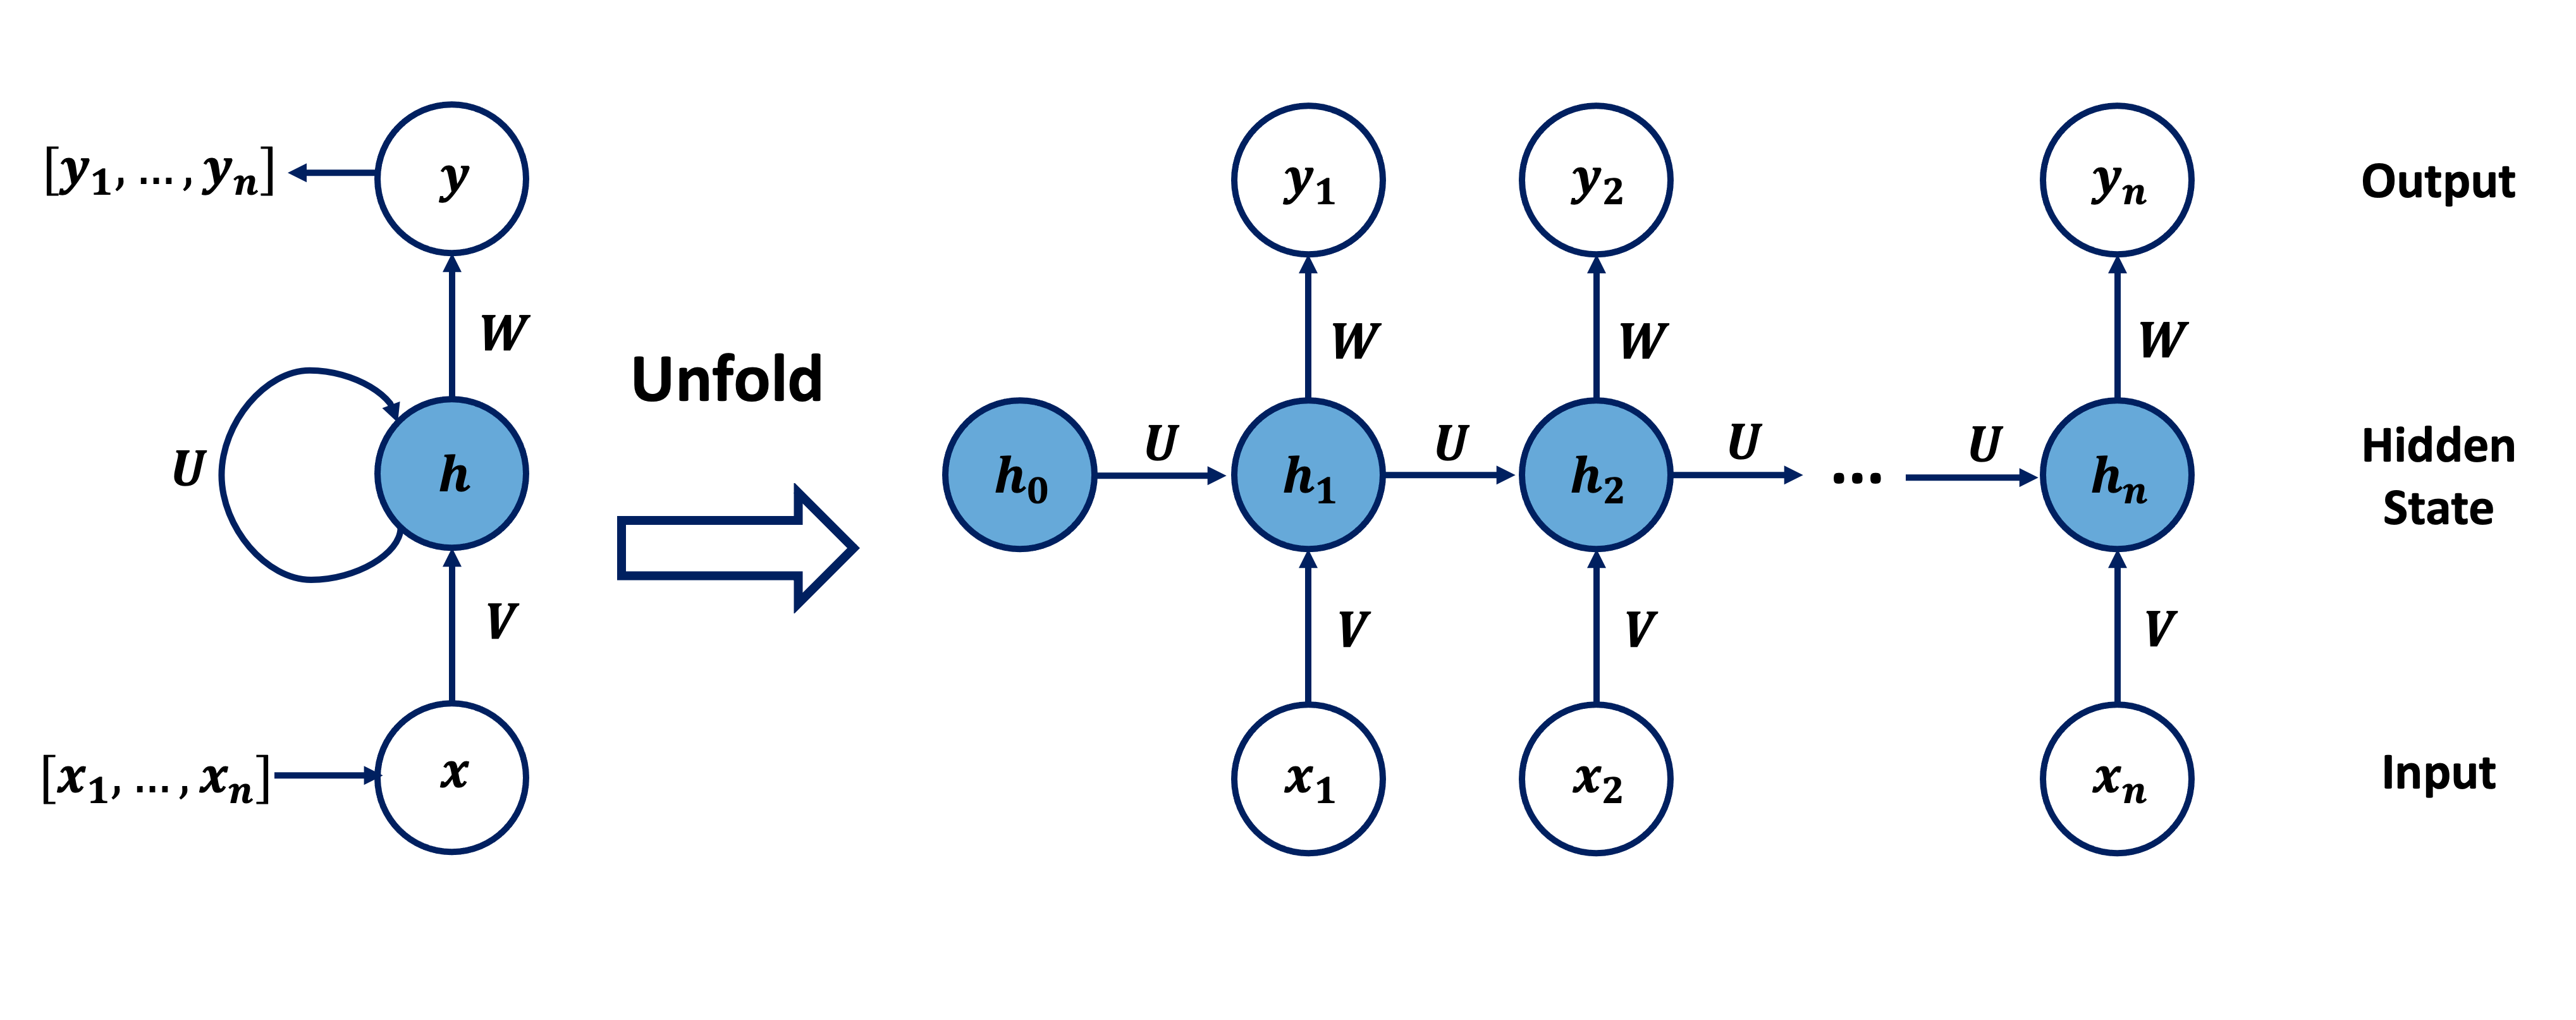
\includegraphics[scale=0.5]{Images/ML/rnn.png}
    \caption{A recurrent neural network, using 3 feed-forward neural networks (DNN) $U$, $V$, $W$, to map the input sequence $x = [x_1, x_2, ..., x_N]$ to the output $y = [y_1, y_2, ..., y_N]$ using the internal hidden state $h^t$ evolving for each timestep $t$. $h_0$ would typically be obtained by a mapping of the whole input sequence $x$. } 
    \label{fig:rnnNet}
\end{figure}

%\subsubsection{Long-Short Term Memory} 
As shown in Figure~\ref{fig:lstmCell}, Long-Short Term Memory (\gls{lstm}) cells implement a specific architecture to propagate information along the sequence, with the introduction of a new control state $c$ \cite{lstmPaper}. Three gates covering the forget, the input, and the output regulate the flow of information from the cell. In particular, the forget gate $F$ decides what information to keep from prior states, by multiplying these values by a factor 1 and discards the rest through a multiplication by a factor close to 0. The input gate $I$ is tasked with creating the new internal state of the cell and what information to store in it. Finally, the output gate $O$ decides what information in the cell should be brought to the output. This selectivity of the \gls{lstm} cell to decide what to use from memory, what to keep in memory, and what to output gives this architecture a far-improved memory for long sequences which results in a much-improved efficiency. 

\begin{figure}[h!]
    \center
    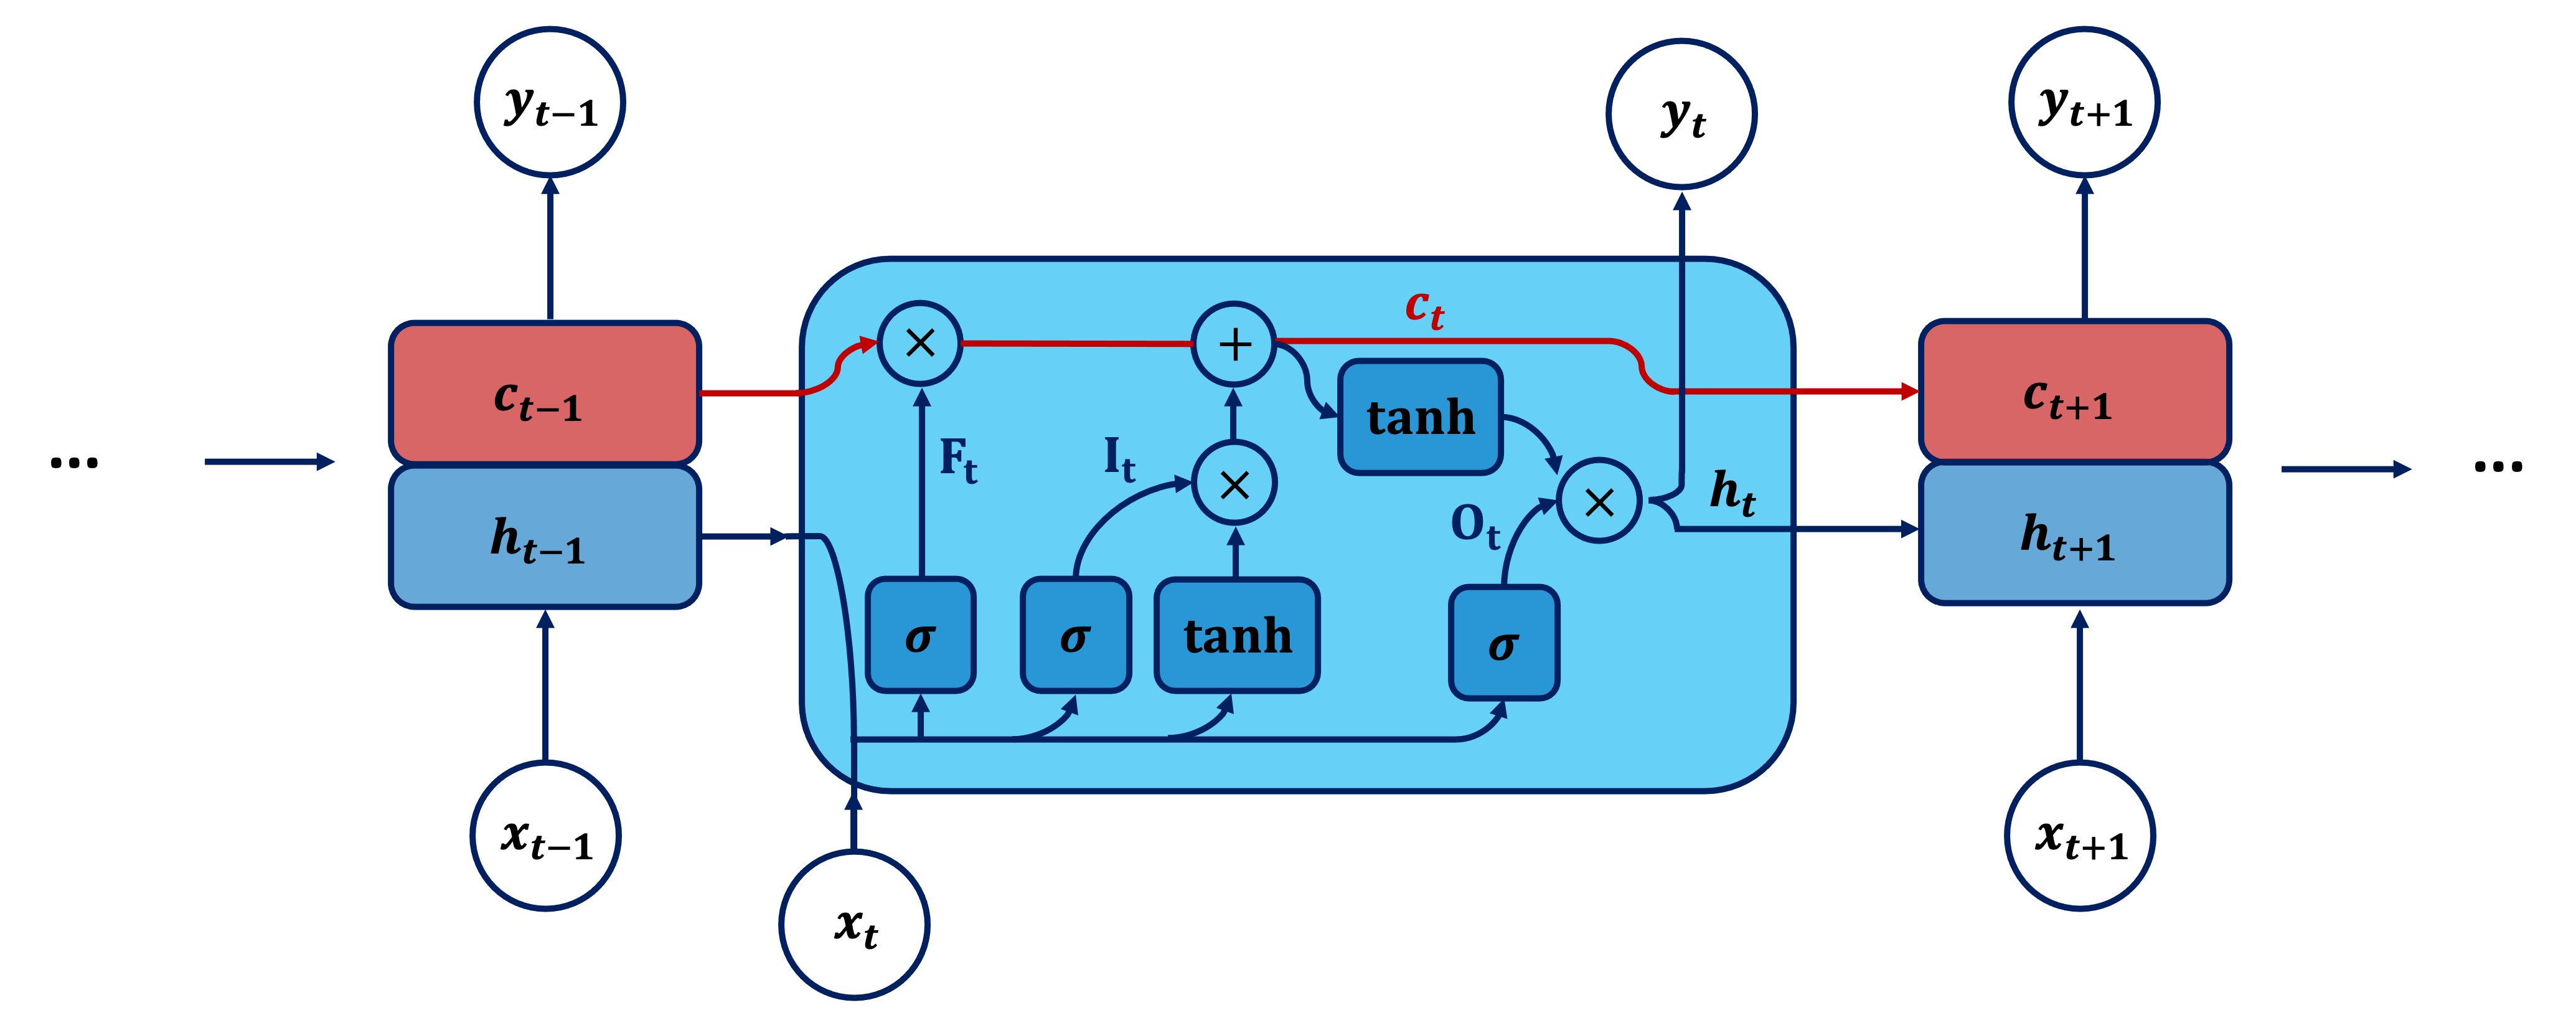
\includegraphics[scale=0.5]{Images/ML/lstm.png}
    \caption{An LSTM cell. Arrows and lines that merge imply concatenation of the inputs, the $\times$, $+$, and tanh are element-wise operations and the $\sigma$ are different layered transformations (1-layer feed-forward network). $F_t$ is the forget gate of the memory cell $c$, $I_t$ the input gate, and $O_t$ the output gate. } 
    \label{fig:lstmCell}
\end{figure}

%\subsubsection{Gated Recurrent Unit} 
%The Gated Recurrent Unit (\gls{gru}) is another advantageous design to improve the %memory of a recurrent-like network without using as many parameters as an \gls{lstm} %\cite{gruPaper}. There is no output gate and only one internal hidden state $h_t$ is %required. This architecture comes in different versions, with the fully gated version %presented in Figure~\ref{fig:gruCell}. It only requires two gates: the \textit{update %gate} $Z$ and the \textit{reset gate} $R$. The former lets the model decide how much of %the past information should be kept and the latter is used to forget past information.
%
%\begin{figure}[h!]
%    \center
%    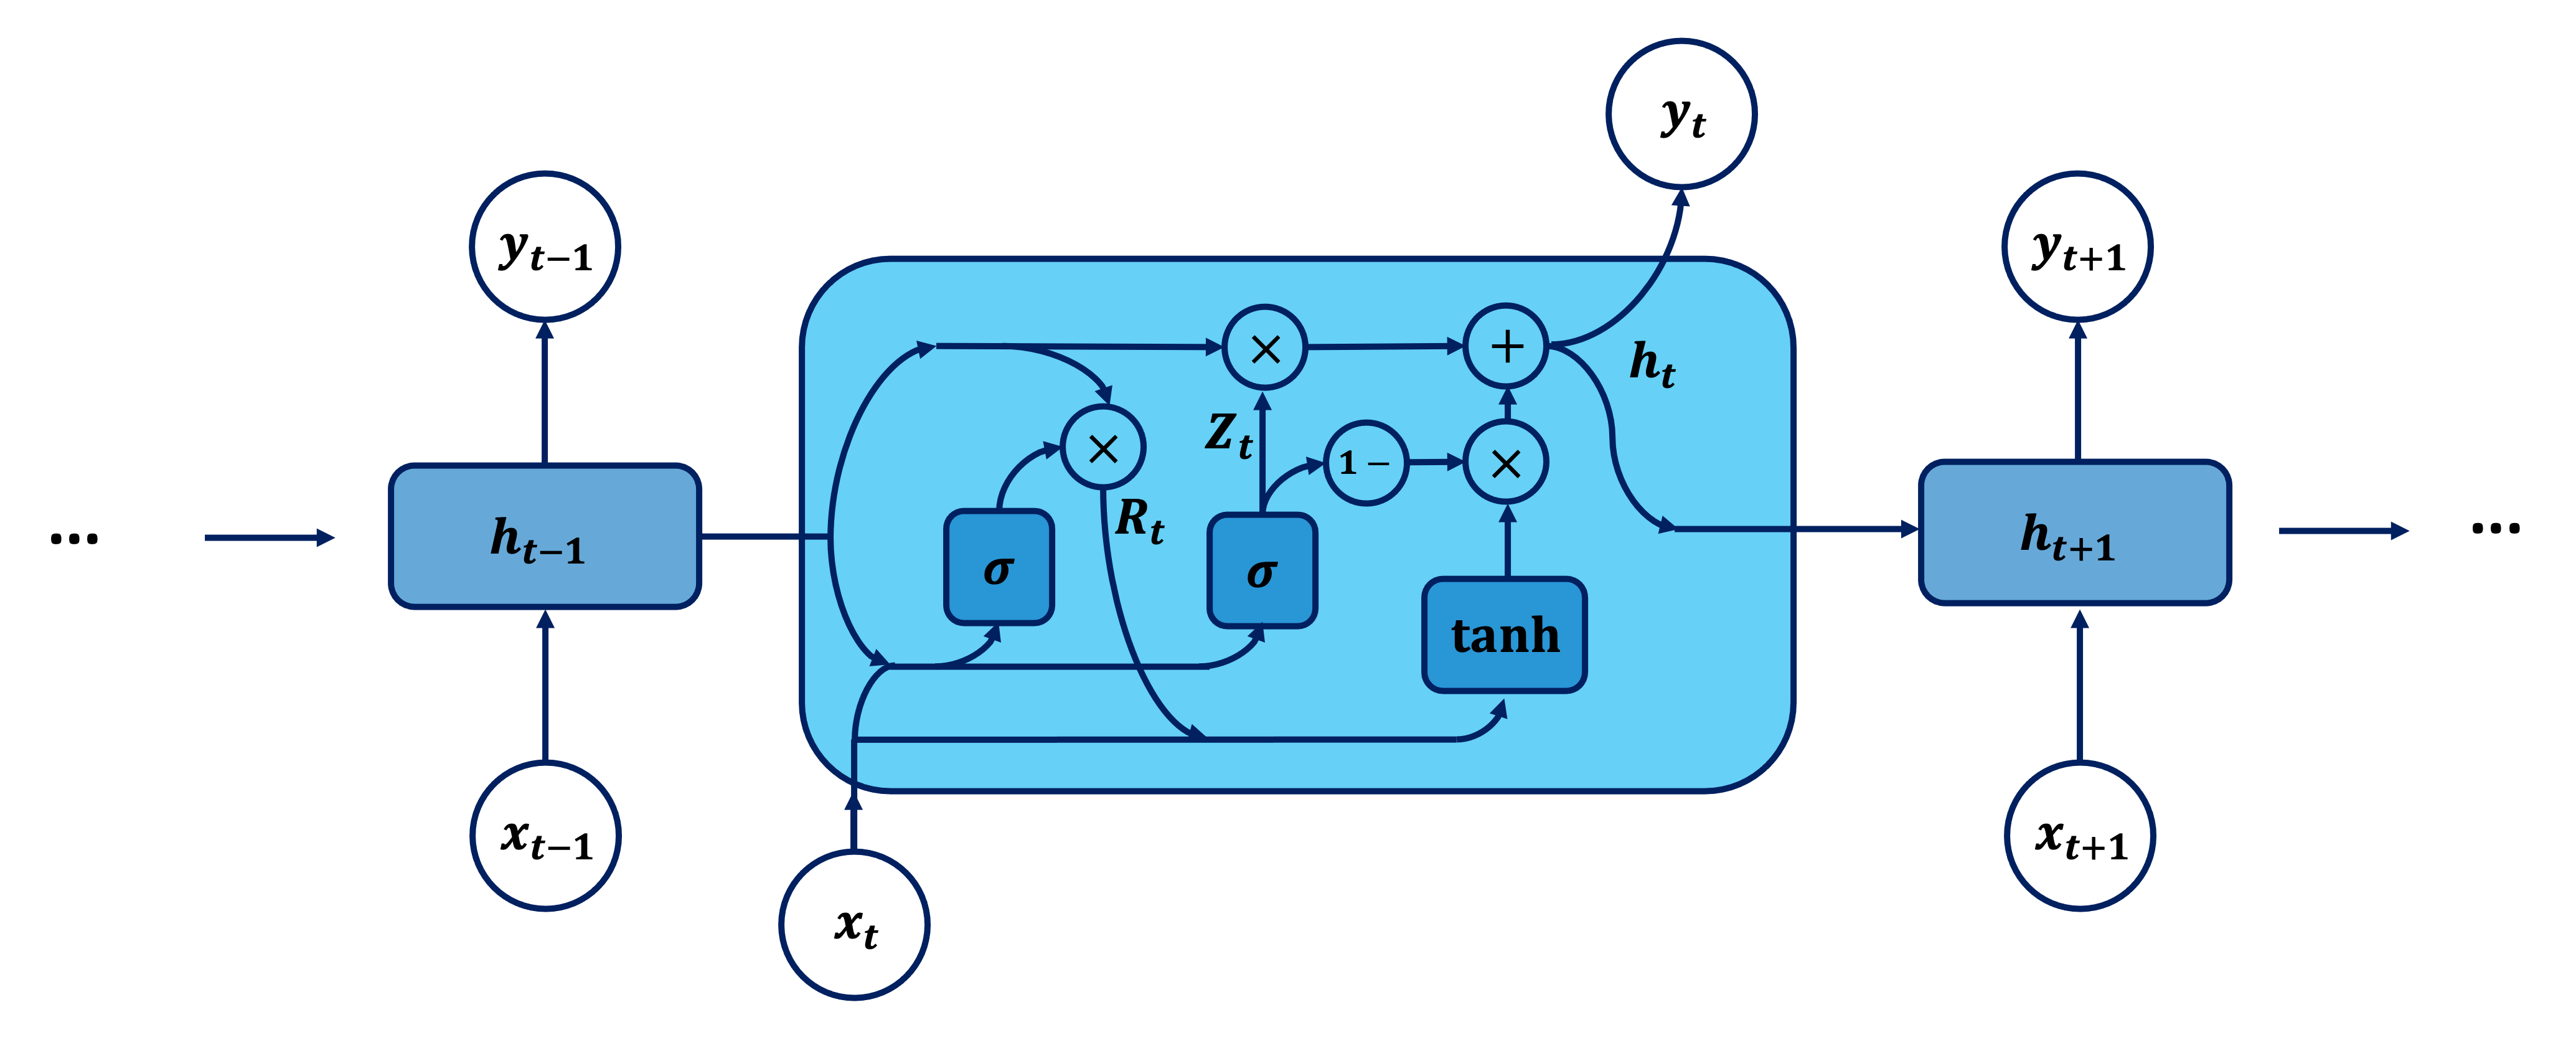
\includegraphics[scale=0.5]{Images/ML/gru.png}
%    \caption{A Gated Recurrent Unit cell (fully-gated version). Arrows and lines that %merge imply concatenation of the inputs, the $\times$, $+$, tanh, and ``1 - '' are %element-wise operations - the last one outputting the vector 1 minus its inputs - %and the $\sigma$ are two different layered transformations (1-layer feed-forward %network) with sigmoid-like activation function. $Z_t$ is the update gate and $R_t$ %the reset gate. } 
%    \label{fig:gruCell}
%\end{figure}

\glspl{rnn} and their modification have been designed for ordered sequence analysis and have had great results in such settings. Ordered sequences are natural in language analysis. The choice to sequentially analyse the tokens of a sequence with memory lets \gls{rnn}-based models operate similarly to Turing Machines, endowing them with the powerful representational flexibility of Universal Turing Machine \cite{NEURIPS2021_ef452c63}. A significant drawback however is the impossibility to fully parallelise the processing of sequence due to the strict ordering, making \gls{rnn} expensive models to train. The main motivation behind the transformer design, introduced in section \ref{sec:transformer}, is to fix this crucial weakness.

\paragraph{Pros:}
\begin{itemize}
    \item \textit{Sequential Processing:} \glspl{rnn} are designed to handle sequential data, making them suitable for tasks with temporal dependencies.
    \item \textit{Flexibility:} \glspl{rnn} can operate on input sequences of variable length.
    \item \textit{Memory:} \glspl{rnn} have a memory mechanism that allows them to retain information about previous inputs.
\end{itemize}

\paragraph{Cons:}
\begin{itemize}
    \item \textit{Vanishing and Exploding Gradients:} Training deep \glspl{rnn} can suffer from vanishing and exploding gradient problems.
    \item \textit{Limited Short-Term Memory:} Traditional \glspl{rnn} struggle to capture long-range dependencies due to their limited short-term memory. 
    \item \textit{Complexity:} While the \gls{lstm} architecture can mitigate the two points above, the cost is a more complex architecture that is harder to train. 
    \item \textit{Interpretability:} The internal workings of a \gls{rnn} is challenging to interpret.
\end{itemize}

\subsection{Convolutional Neural Networks}
Convolutional Neural Networks (\gls{cnn}) \cite{NIPS198953c3bce6, NIPS2012_c399862d} have emerged as a powerful class of deep learning models that are particularly effective in computer vision tasks, including image and video analysis. The architecture consists of convolutional layers - implementing the fundamental convolution operation-, pooling layers, and \glspl{dnn}. This architecture, presented in Figure~\ref{fig:cnnDesign}, enables \gls{cnn} to automatically learn hierarchical representations of features while respecting properties of image-based data: spaciality (pixels have a position), locality (pixel share information within their neighbourhood), and symmetries.

\begin{figure}[h!]
    \center
    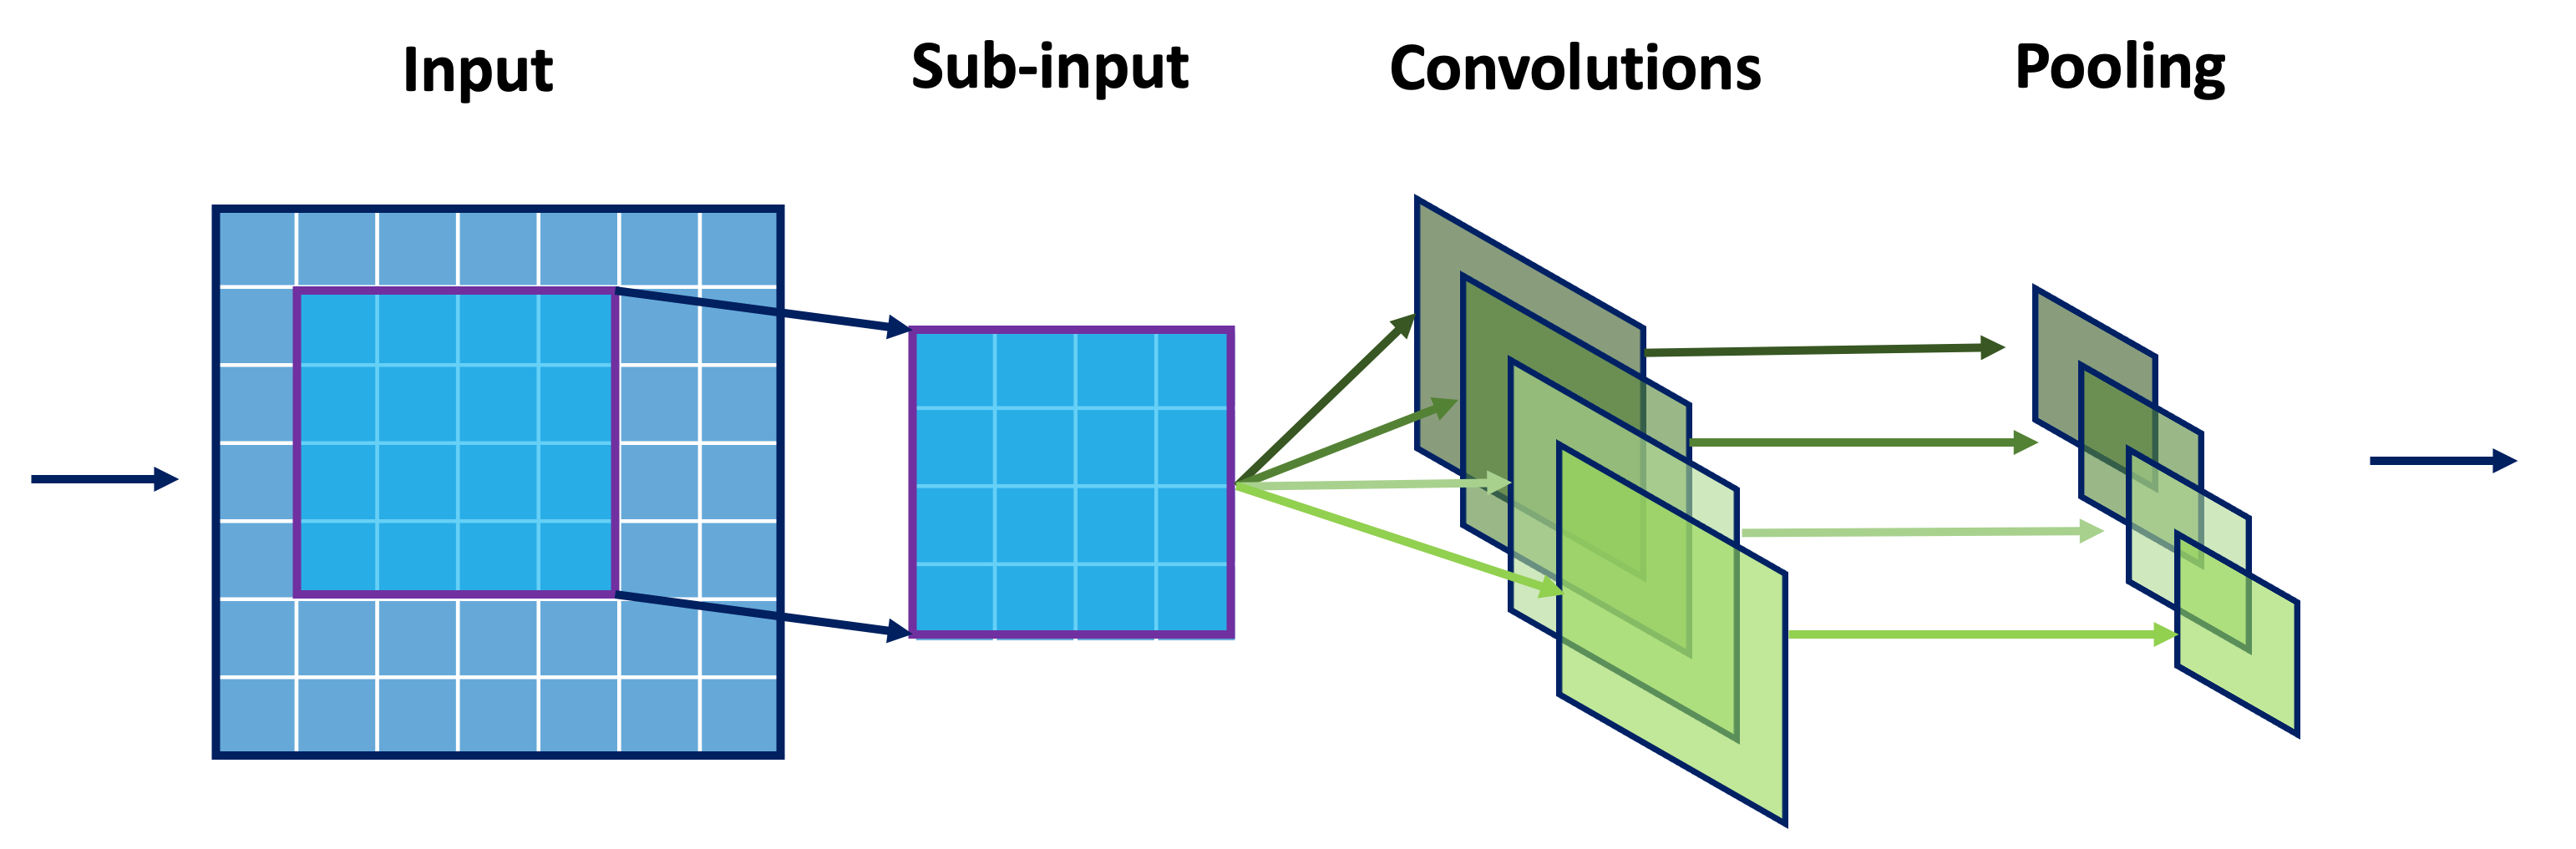
\includegraphics[width=0.9\textwidth]{Images/ML/cnn.png}
    \caption{A layer of a convolutional neural network, implementing a convolution with 4 kernels followed by a pooling operation. This design can be stacked to create deep architecture, and combined with a feed-forward neural network, after flattening the output at some depth, before reaching the final loss function layer.} 
    \label{fig:cnnDesign}
\end{figure}

The \gls{cnn} leverage convolutional layers to extract local patterns and features from input data. Convolutional operations are applied to the input data by multiplying entry-by-entry a learnable \textit{kernel} or \textit{filter}, represented by a matrix of weights of smaller dimension than the total image size, with an equal size subpart of the input and applying an activation function. The size of the filter or kernel restricts the processing of the input to a given \textit{receptive field} dimension, and this window is passed over the full input image by moving it by a defined \textit{stride} length. Pooling layers are then used to reduce spatial dimensions and retain important features. This process is parallelisable for an image with multiple channels. For classification and regression, a \gls{cnn} typically stacks several convolutional and pooling layers before leading to a fully connected neural network ``flattening'' the last representation to make predictions. \textit{Flattening} refers to the process of transforming the input image, represented as a matrix $\mathbb{R}^{x} \times \mathbb{R}^{y}$, into a vector $\mathbb{R}^{x \times y}$. \\

\gls{cnn}-based models, such as AlexNet \cite{NIPS2012_c399862d} and ResNet \cite{resNetPaper}, have demonstrated state-of-the-art performance in various computer vision tasks. A main advantage of the convolution operation on an image of size $x \times y$ is the reduction of the number of artificial neurons required to process the image, which helps to regularise the network. For a given image:
\begin{itemize}
    \item A \gls{dnn} given the flatten the image requires $x \times y$ neurons. 
    \item A \gls{cnn} with $k$ kernels of size $\alpha \times \beta$ requires $k \times \alpha \times \beta$ artificial neurons. 
\end{itemize}
For example, for an image of size 100 $\times$ 100, a \gls{dnn} requires 10,000 neurons while a \gls{cnn} can process the image with only 25 units if a single kernel of size 5 $\times$ 5 is used. Typical pooling functions are the \textit{maxPooling} or the \textit{sumPooling}, which, respectively, take the largest element or the sum in each window of their input, with specific hyperparameters governing the size and the movements of the window.

\paragraph{Pros:}
\begin{itemize}
    \item \textit{Feature Learning:} \glspl{cnn} automatically learn hierarchical representations of features on multidimensional data.
    \item \textit{Spatial Hierarchies:} convolutional and pooling layers enable the model to capture spatial hierarchies in the input data while respecting the properties of images. 
    \item \textit{State-of-the-Art Performance:} \glspl{cnn} have achieved state-of-the-art performance in image classification, object detection, and segmentation tasks.
\end{itemize}

\paragraph{Cons:}
\begin{itemize}
    \item \textit{Computational Complexity:} training deep \glspl{cnn} is computationally intensive.
    \item \textit{Large Datasets:} \gls{cnn} often require large datasets for effective training.
    \item \textit{Interpretability:} The internal workings of \glspl{cnn} are challenging to interpret.
\end{itemize}

\subsection{Graph Neural Networks}\label{chapter-GNN}
Recentely, \glspl{gnn} have garned attention for their ability to model and analyse complex relationships within graph-structured data \cite{graphNetRef}. Originally designed for tasks such as node classification and link prediction, \glspl{gnn} have found applications in diverse domains such as social networks modelling, recommendation systems, and physics, for modelling the dynamic of a $N$-body system, performing tracks reconstruction, and identifying particles. \glspl{gnn} operate on graph-structured data, where nodes or vertices represent entities, and edges represent relationships between these entities. The functioning of \glspl{gnn} involves iterative aggregation of information from neighbouring nodes and updating of the edges, allowing them to capture both local and global structures defined by the graph. An interesting feature of graphs is that the input information does not need to be given a rigid structure. Consequently, graph-based methods have a much greater representation power than image- or sequence-based ones. Graphs are in fact able to represent arbitrary relational structures, as defined by directional weighted edges \cite{graphInductiveBias}. A particular feature arising from this property is that graphs are permutation equivariant: the order of nodes can be rearranged without impact. \\

\begin{figure}[h!]
    \center
    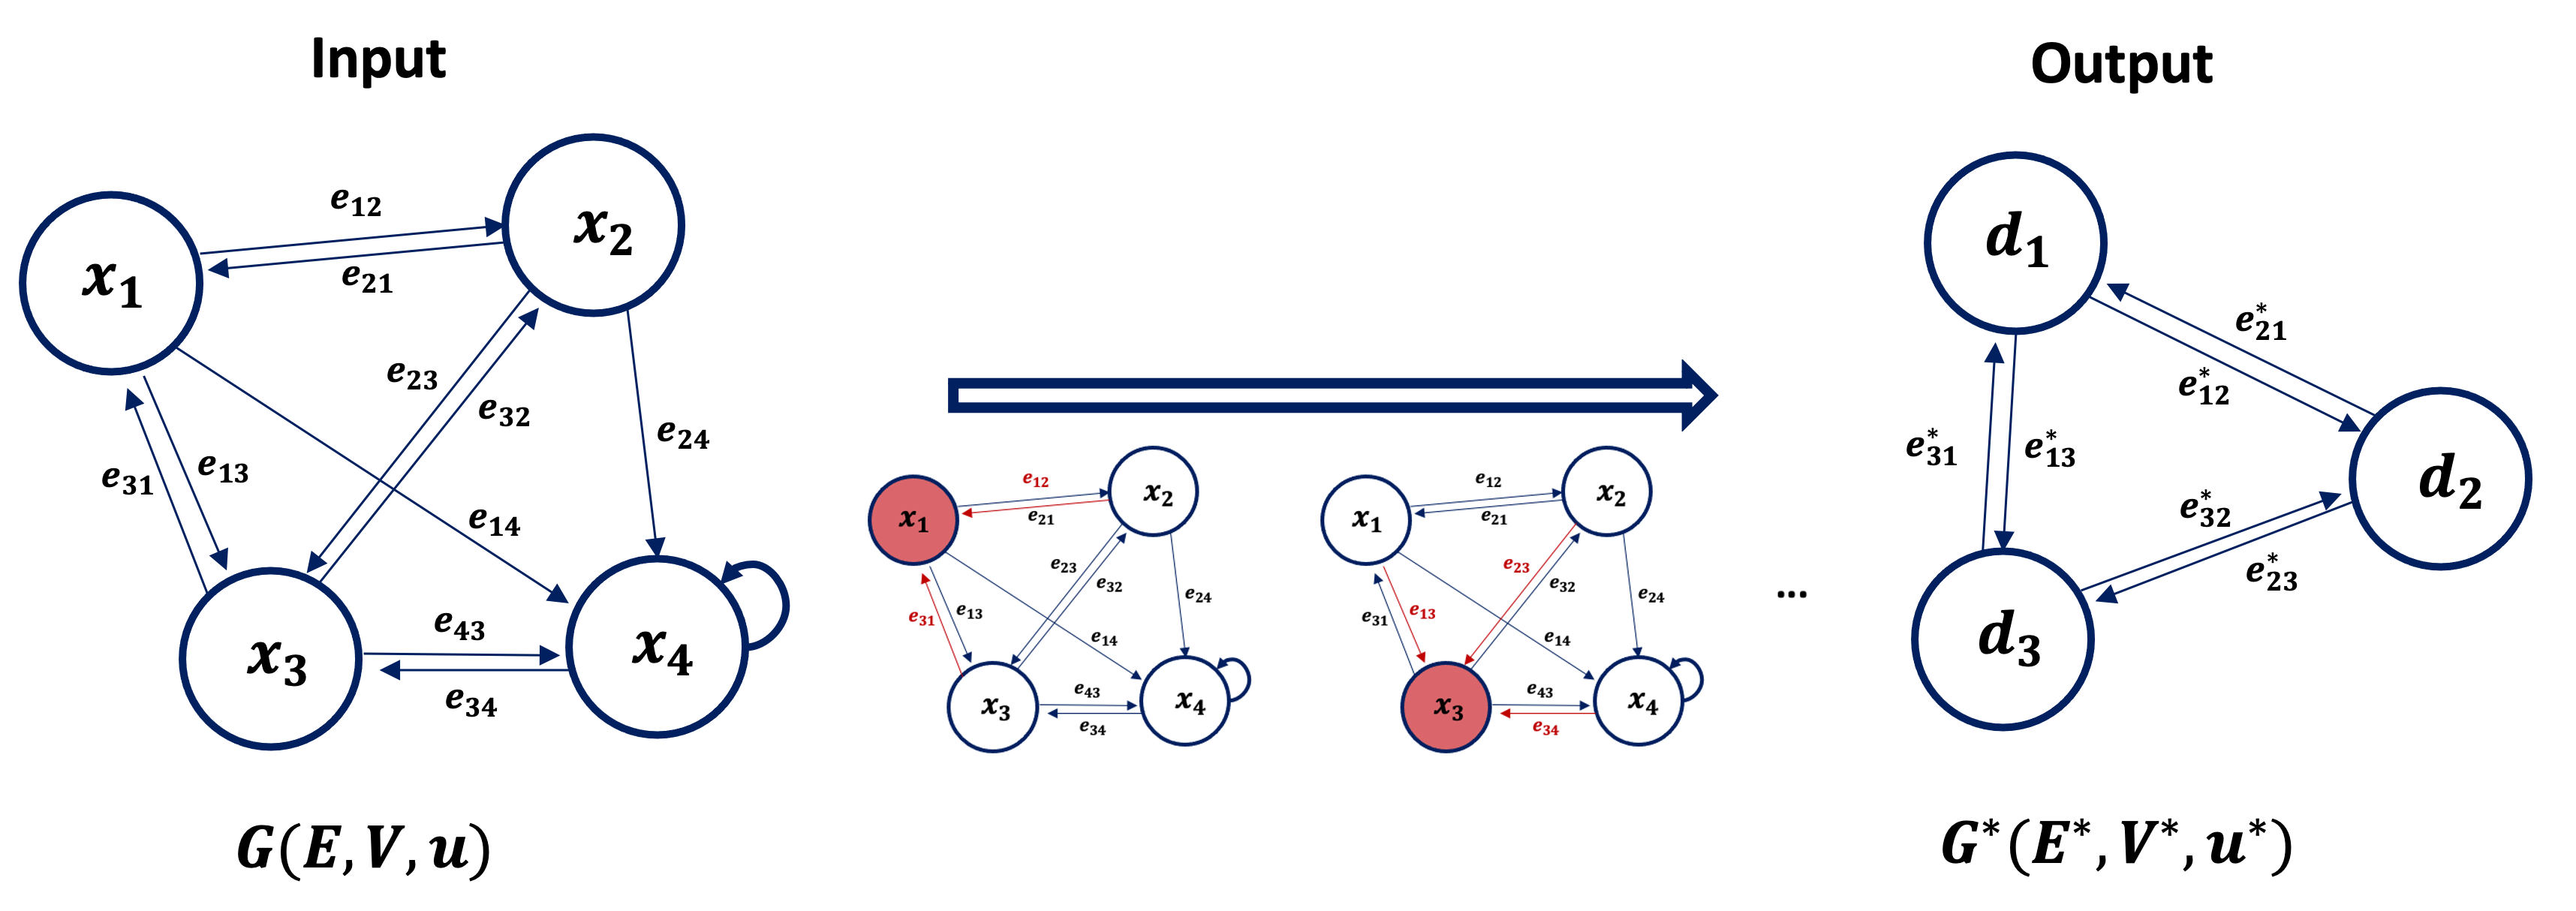
\includegraphics[width=\textwidth]{Images/ML/gnn.png}
    \caption{A graph neural network update on a directed graph $G(V, E, u)$ with a global representation $u$, four initial nodes $\in V$ and edges $e_{ij} \in E$ connecting nodes $i \rightarrow j$. By analysing the neighbours of each node, the graph is updated to a new graph $G^*(V^*, E^*, u^*)$.} %(in the notation of the text, each node is given a different integer index $k$ and written $(e_k, r_k, s_k)$, with $r_k = j$ and $s_k = i$)
    \label{fig:gnnScheme}
\end{figure}

A \gls{gnn} architecture consists of multiple layers of message-passing operations. Each layer updates the node representations by aggregating information from neighbouring nodes, as schematised in Figure~\ref{fig:gnnScheme}. Different architectures implement different update processes for the graph, with popular \gls{gnn} architectures being Graph Convolutional Networks (GCNs) \cite{gcnPaper} and Graph Attention Network \cite{velickovic2018graph}. In this thesis, the notation adopted is to represent a graph $G$ has a tuple of three integers:
\begin{enumerate}
    \item $E = \{(e_k, r_k, s_k)\}_{k=1:N^e}$ the set of edges, with each edge having a real vector of features $e_k \in \mathbb{R}^e$ and storing the index of the receiver (sender) as $r_k$ ($s_k$).
    \item $V = \{v\}_{i=1:N^v}$ the set of nodes, each node having a real vector of features $v_i \in \mathbb{R}^v$.
    \item $u$, a global attribute of the graph modelled by a real vector of features $u \in \mathbb{R}^u$. 
\end{enumerate}

\begin{algorithm}
    \caption{Steps of Computation in a Full Graph Network Block \cite{graphInductiveBias}}
    \label{algo:graph_network}
    \begin{algorithmic}[1]
    \Function{GraphNetworkUpdate}{$E, V, u$}
        \For{$k \in \{1 \ldots N^e\}$}
            \State $e^*_k \gets \phi^e(e_k, v_{r_k}, v_{s_k}, u)$
        \EndFor

        \For{$i \in \{1 \ldots N^n\}$}
            \State Let $E_i^* = \{(e^*_k, r_k, s_k)\}$ for $k = 1 : N^e$ where $r_k = i$
            \State $\overline{e^*_i} \gets \rho^{e \to v}(E^*_i)$
            \State $v^*_i \gets \phi^v(\overline{e^*_i}, v_i, u)$
        \EndFor

        \State Let $V^* = \{v^*\}_{i=1}^{N^v}$
        \State Let $E^* = \{(e^*_k, r_k, s_k)\}_{k=1}^{N^e}$
        \State $\overline{e^*} \gets \rho_{e \to u}(E^*)$
        \State $\overline{v^*} \gets \rho_{v \to u}(V^*)$
        \State $u^* \gets \phi_u(\overline{e^*}, \overline{v^*}, u)$

        \State \Return $(E^*, V^*, u^*)$
    \EndFunction
    \end{algorithmic}
\end{algorithm}

The most general graph update algorithm to describe an update stage of a full \gls{gnn} block is described in Algorithm \ref{algo:graph_network}. Essentially, for a given step the input is a graph $G(E, V, u)$ that is updated into a new graph $G^*(E^*, V^*, u^*)$ by first updating the edges $e \in E$, then modifying the nodes $v \in V$, and finally the global representation $u$. The update rule leverages different neural networks $\phi$ and aggregation function $\rho$. The aggregation function must accept a variable number of inputs with permutation invariance to output a single element per group and is typically implemented with the sum or max pooling. This global update is decomposed into successive steps: 
\begin{itemize}
    \item Updates the edges, with a \gls{dnn} $\phi^e$ mapping each of the input edges, their respective receiver and sender nodes, and the global state $u$ to output a new edge feature vector $e^*_k$ for each edge $k$: $e^*_k = \phi^e(e_k, v_{r_k}, v_{s_k}, u)$. The new edges are stored in a set $E^*$. 
    \item Before updating a vertex $i$ represented by $v_i$, the $E_i^*$ updated edges connecting to $i$ are pooled locally over the node as $\overline{e^*_i} = \rho^{e \rightarrow v}(E_i^*)$.
    \item The vertex is then updated with a \gls{dnn} $\phi^v$ mapping the pooled representation of the edges $\overline{e^*_i}$ connected to the vertex being updated, the input vertex feature $v_i$, and the global representation $u$ to update $v_i \rightarrow v^*_i = \phi^v(\overline{e^*_i}, v_i, u)$. The new vertices are stored in $V^*$.
    \item The set of edges is updated by a global pooling $\overline{e^*} = \rho^{e \rightarrow u}(E^*)$.
    \item The set of vertices is updated by a global pooling $\overline{v^*} = \rho^{v \rightarrow u}(V^*)$.
    \item The global representation is updated by \gls{dnn} $\phi^u$ mapping $u^* = \phi^u(\overline{e^*}, \overline{v^*}, u)$, with the globally pooled updated edges ($\overline{e^*}$) and vertices ($\overline{v^*}$). 
\end{itemize} 
This formulation of a graph as a message-passing with edges update device is the most complete architecture of a \gls{gnn}. The design is however flexible: for example, \glspl{rnn} or \glspl{cnn} can be used instead of \glspl{dnn}. Furthermore, many specialisations of the structures exist to reduce the degree of complexity of the model and avoid overfitting or convergence issues, as listed in Figure~\ref{fig:diverseGNN}. A notable example for this thesis is the Deep Set architecture \cite{NIPS2017f22e4747}, designed to run specifically on sets where the ordering does not matter. It essentially simplifies the graph network by dropping altogether the edges and considering instead a fully connected graph with static edges, with an update of the global representation only based on pooled node information: 
\[v^*_i = \phi^v(\overline{e^*_i}, v_i, u) = \phi^v(v_i, u),\] 
\[\overline{V^*} = \rho^{v \rightarrow u} = \sum_i v^*_i,\] 
\[u^* = \phi^u(\overline{e^*}, \overline{v^*}, u) = \phi^u( \overline{v^*}, u).\] This is somewhat similar to PointNet, a \gls{gnn} designed to analyse sets of 3D points, that uses an analogous update with max-aggregation instead of sum pooling after updating the nodes in two steps \cite{pointNet}.  

\begin{figure}[h!]
    \centering
    \begin{subfigure}[b]{0.49\textwidth}
        \centering
        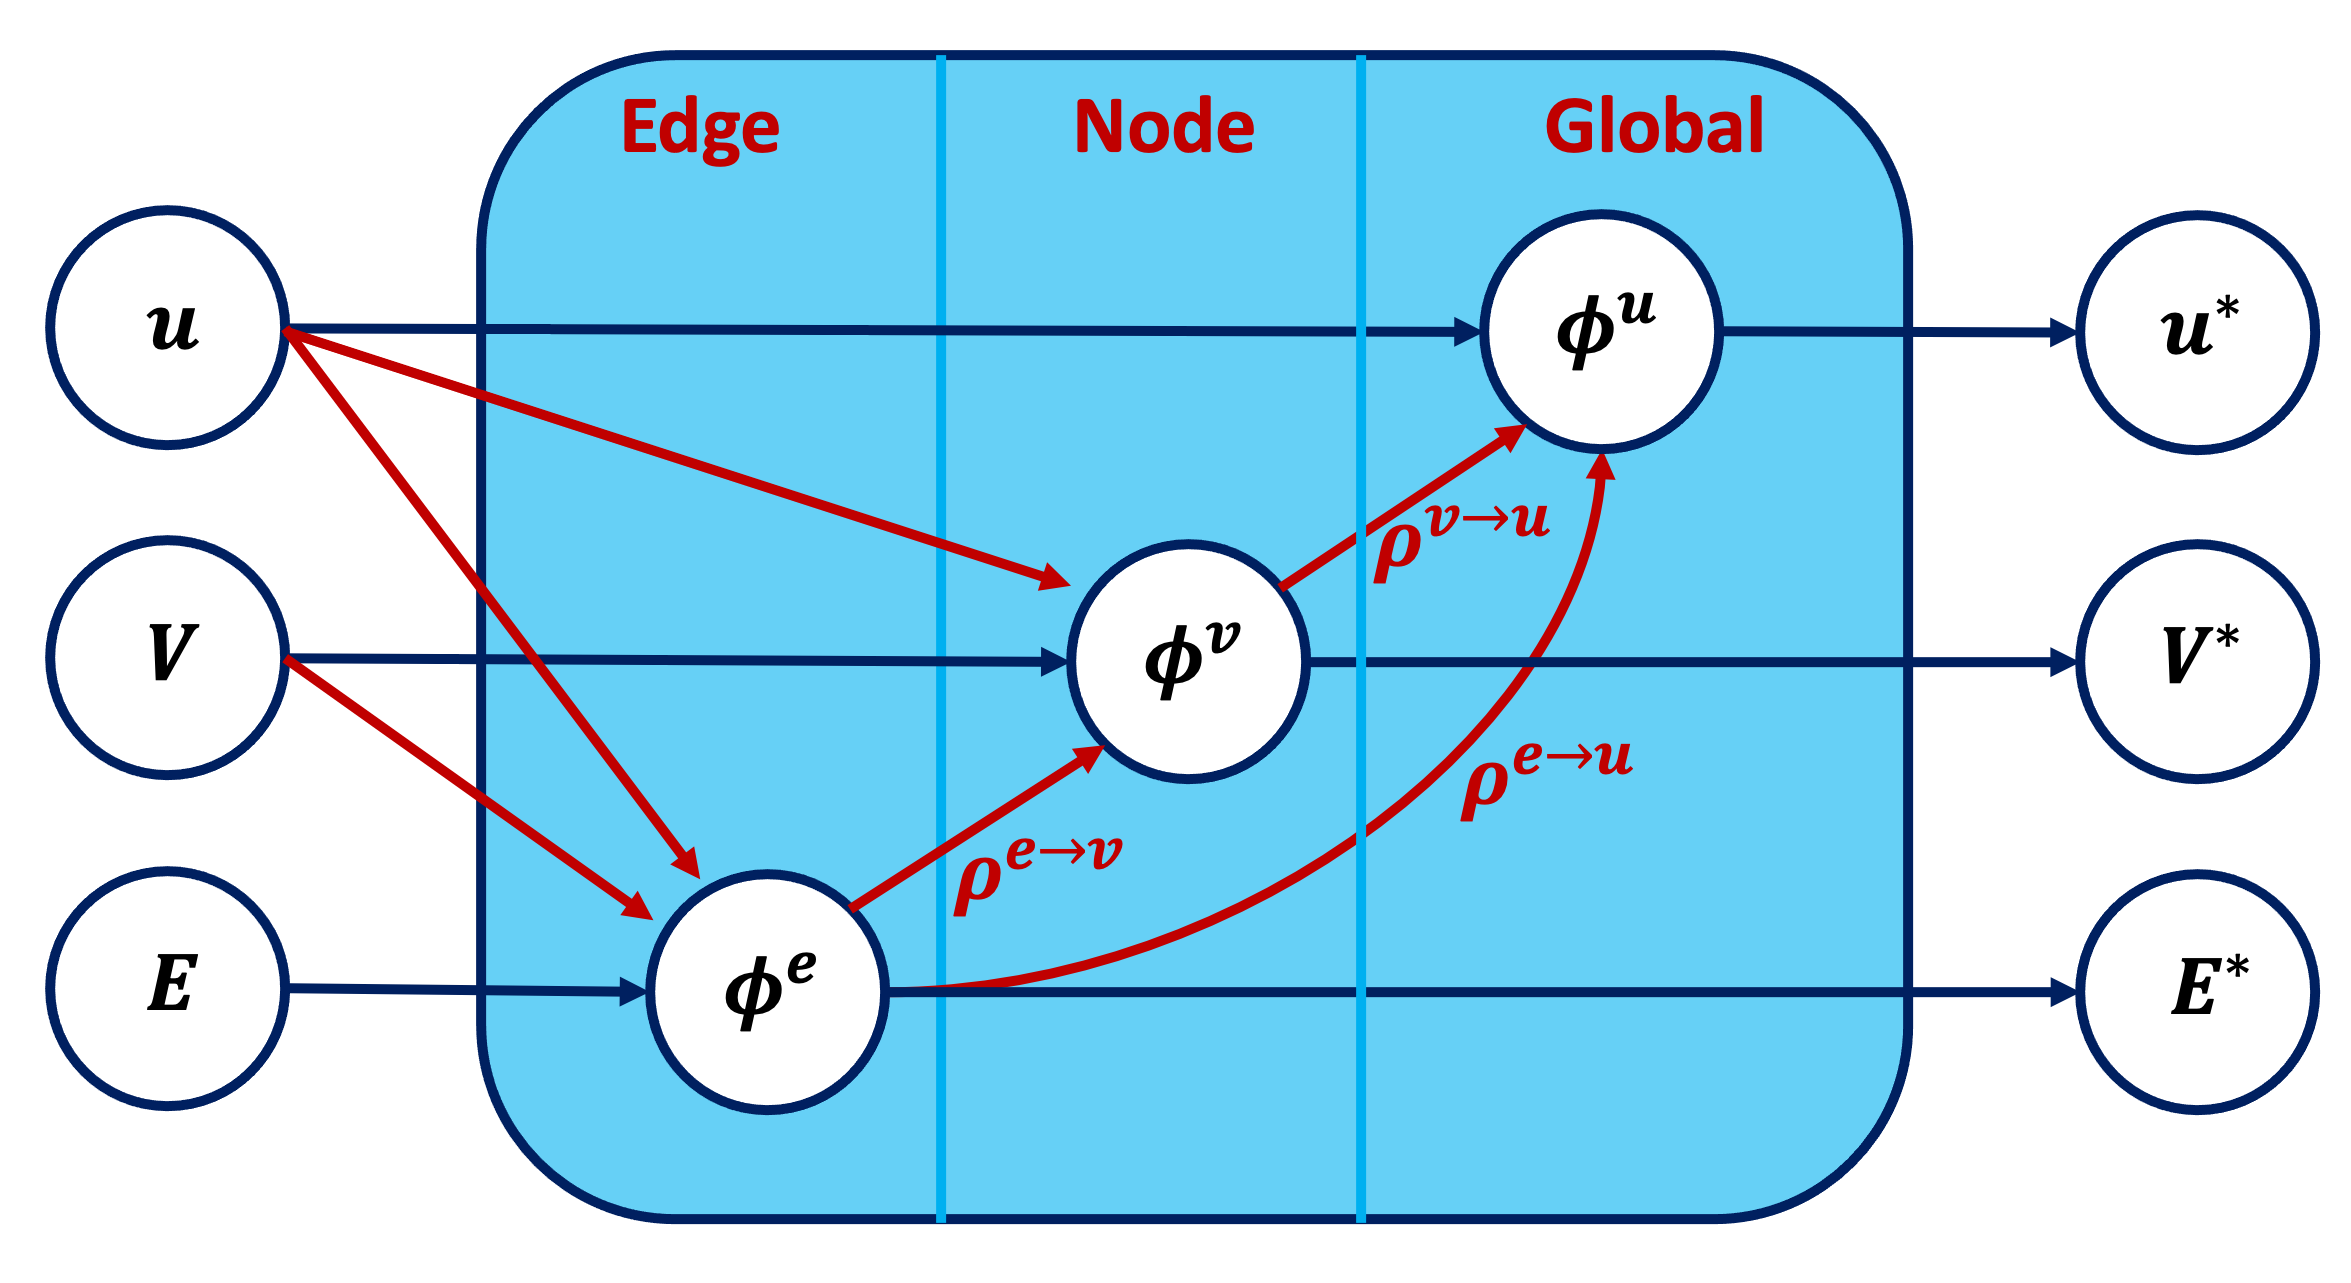
\includegraphics[scale=0.43]{Images/ML/fullGNN.png}
        \caption{Full \gls{gnn}.} 
        \label{fig:diverseGNNfull}
    \end{subfigure}
    \hfill
    \begin{subfigure}[b]{0.49\textwidth}
        \centering
        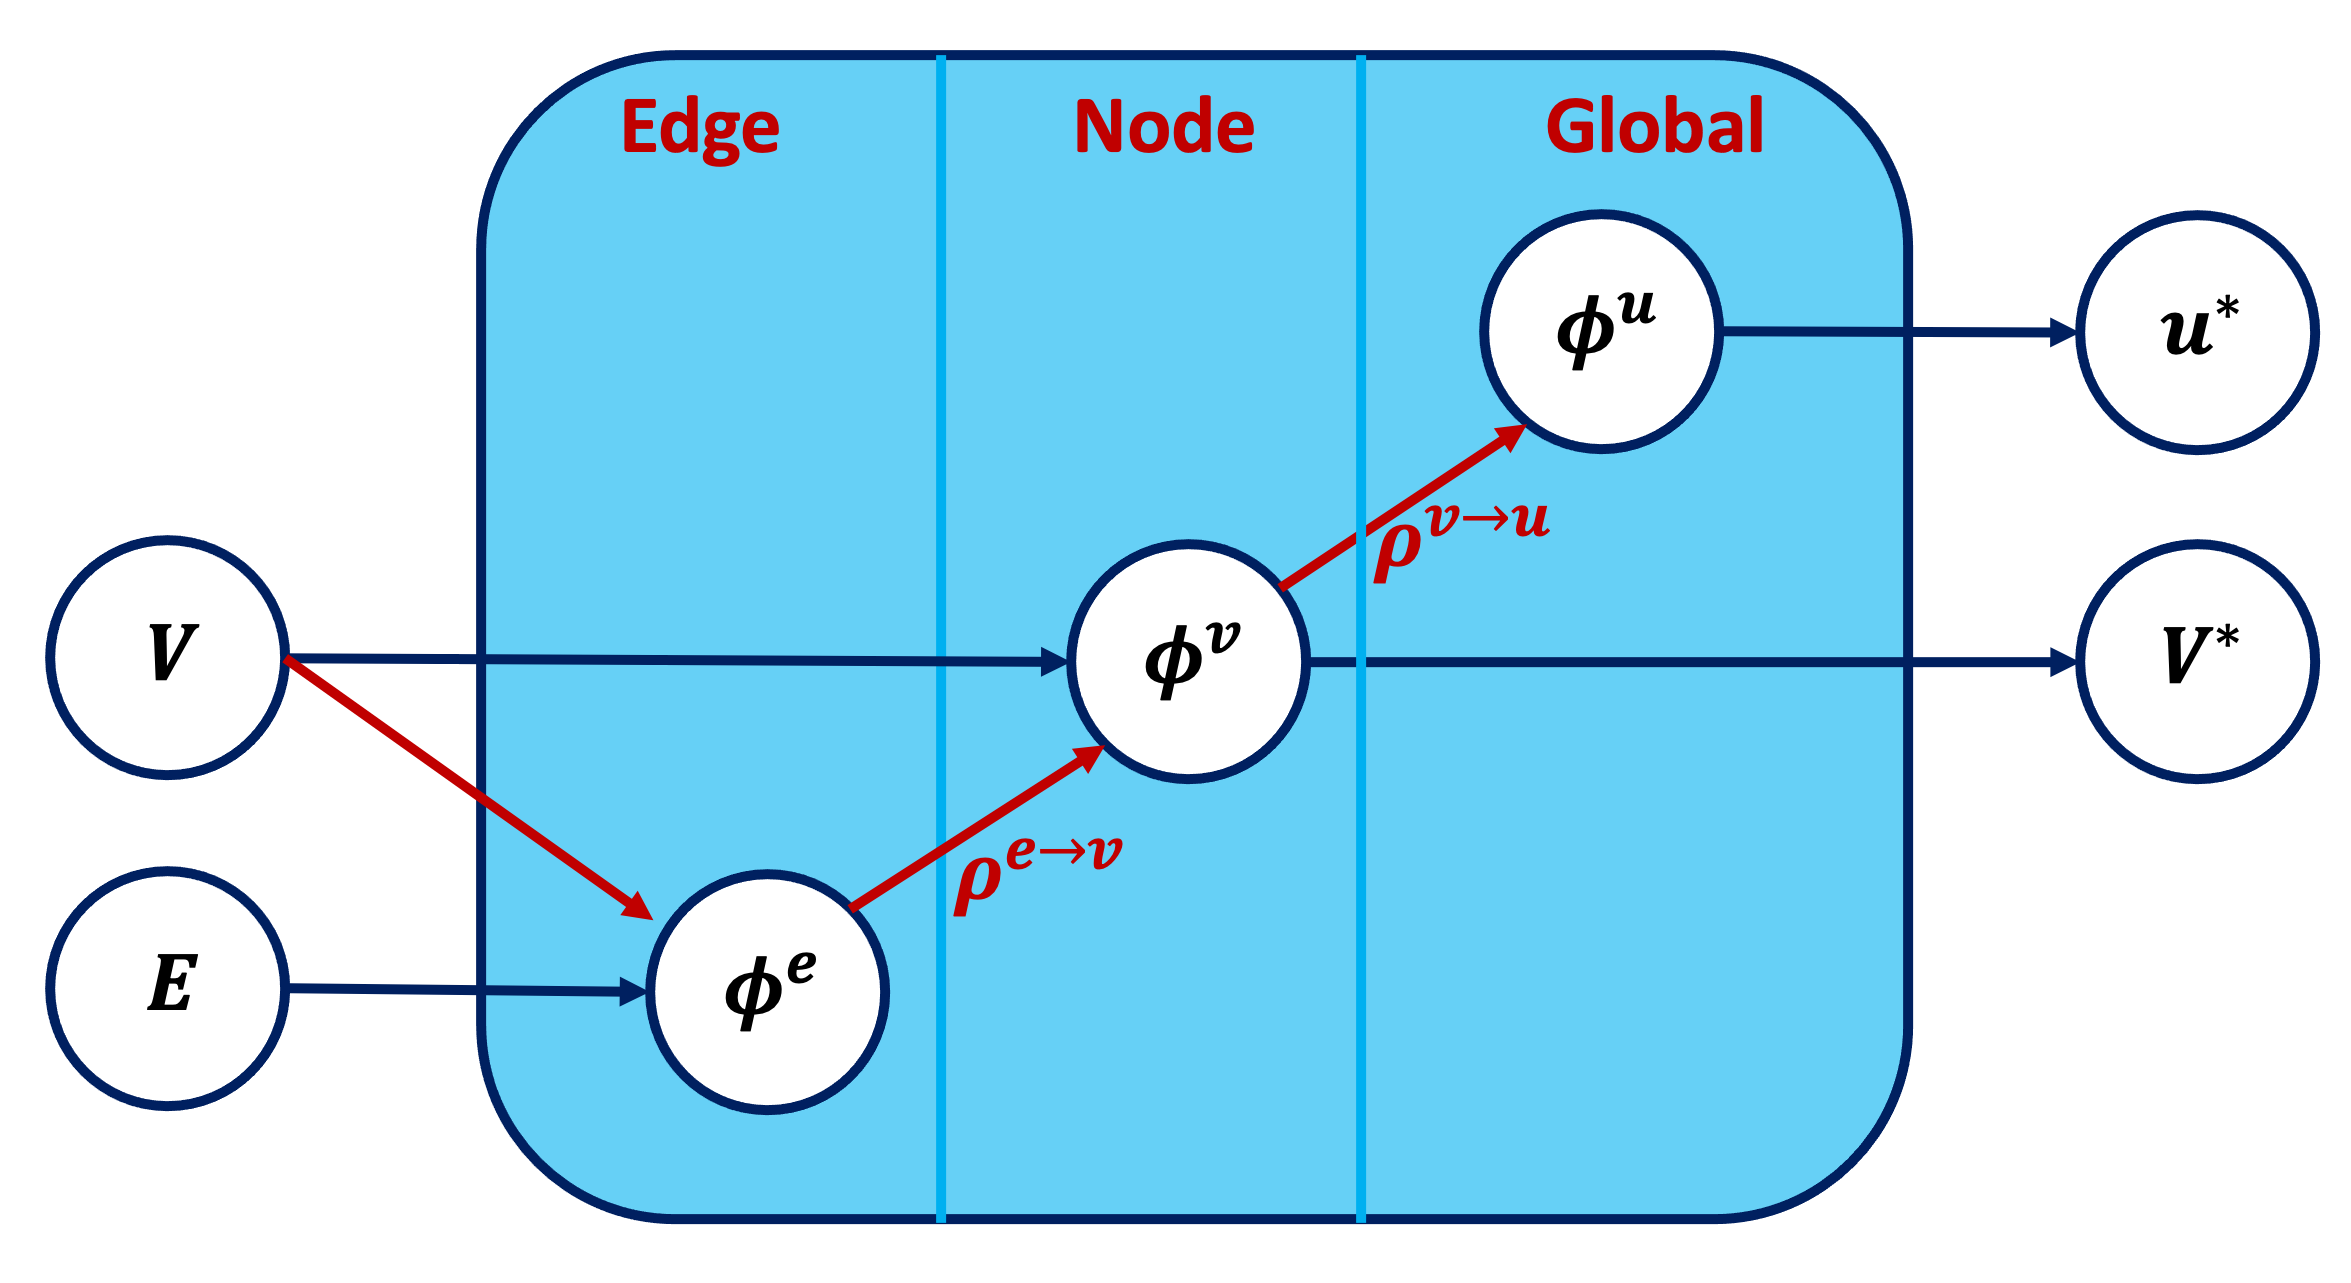
\includegraphics[scale=0.43]{Images/ML/messagepassingNN.png}
        \caption{Message-passing \gls{gnn}.} 
        \label{fig:pullsFTAGmp}
    \end{subfigure}
    \\  % newline
    \begin{subfigure}[b]{0.49\textwidth}
        \centering
        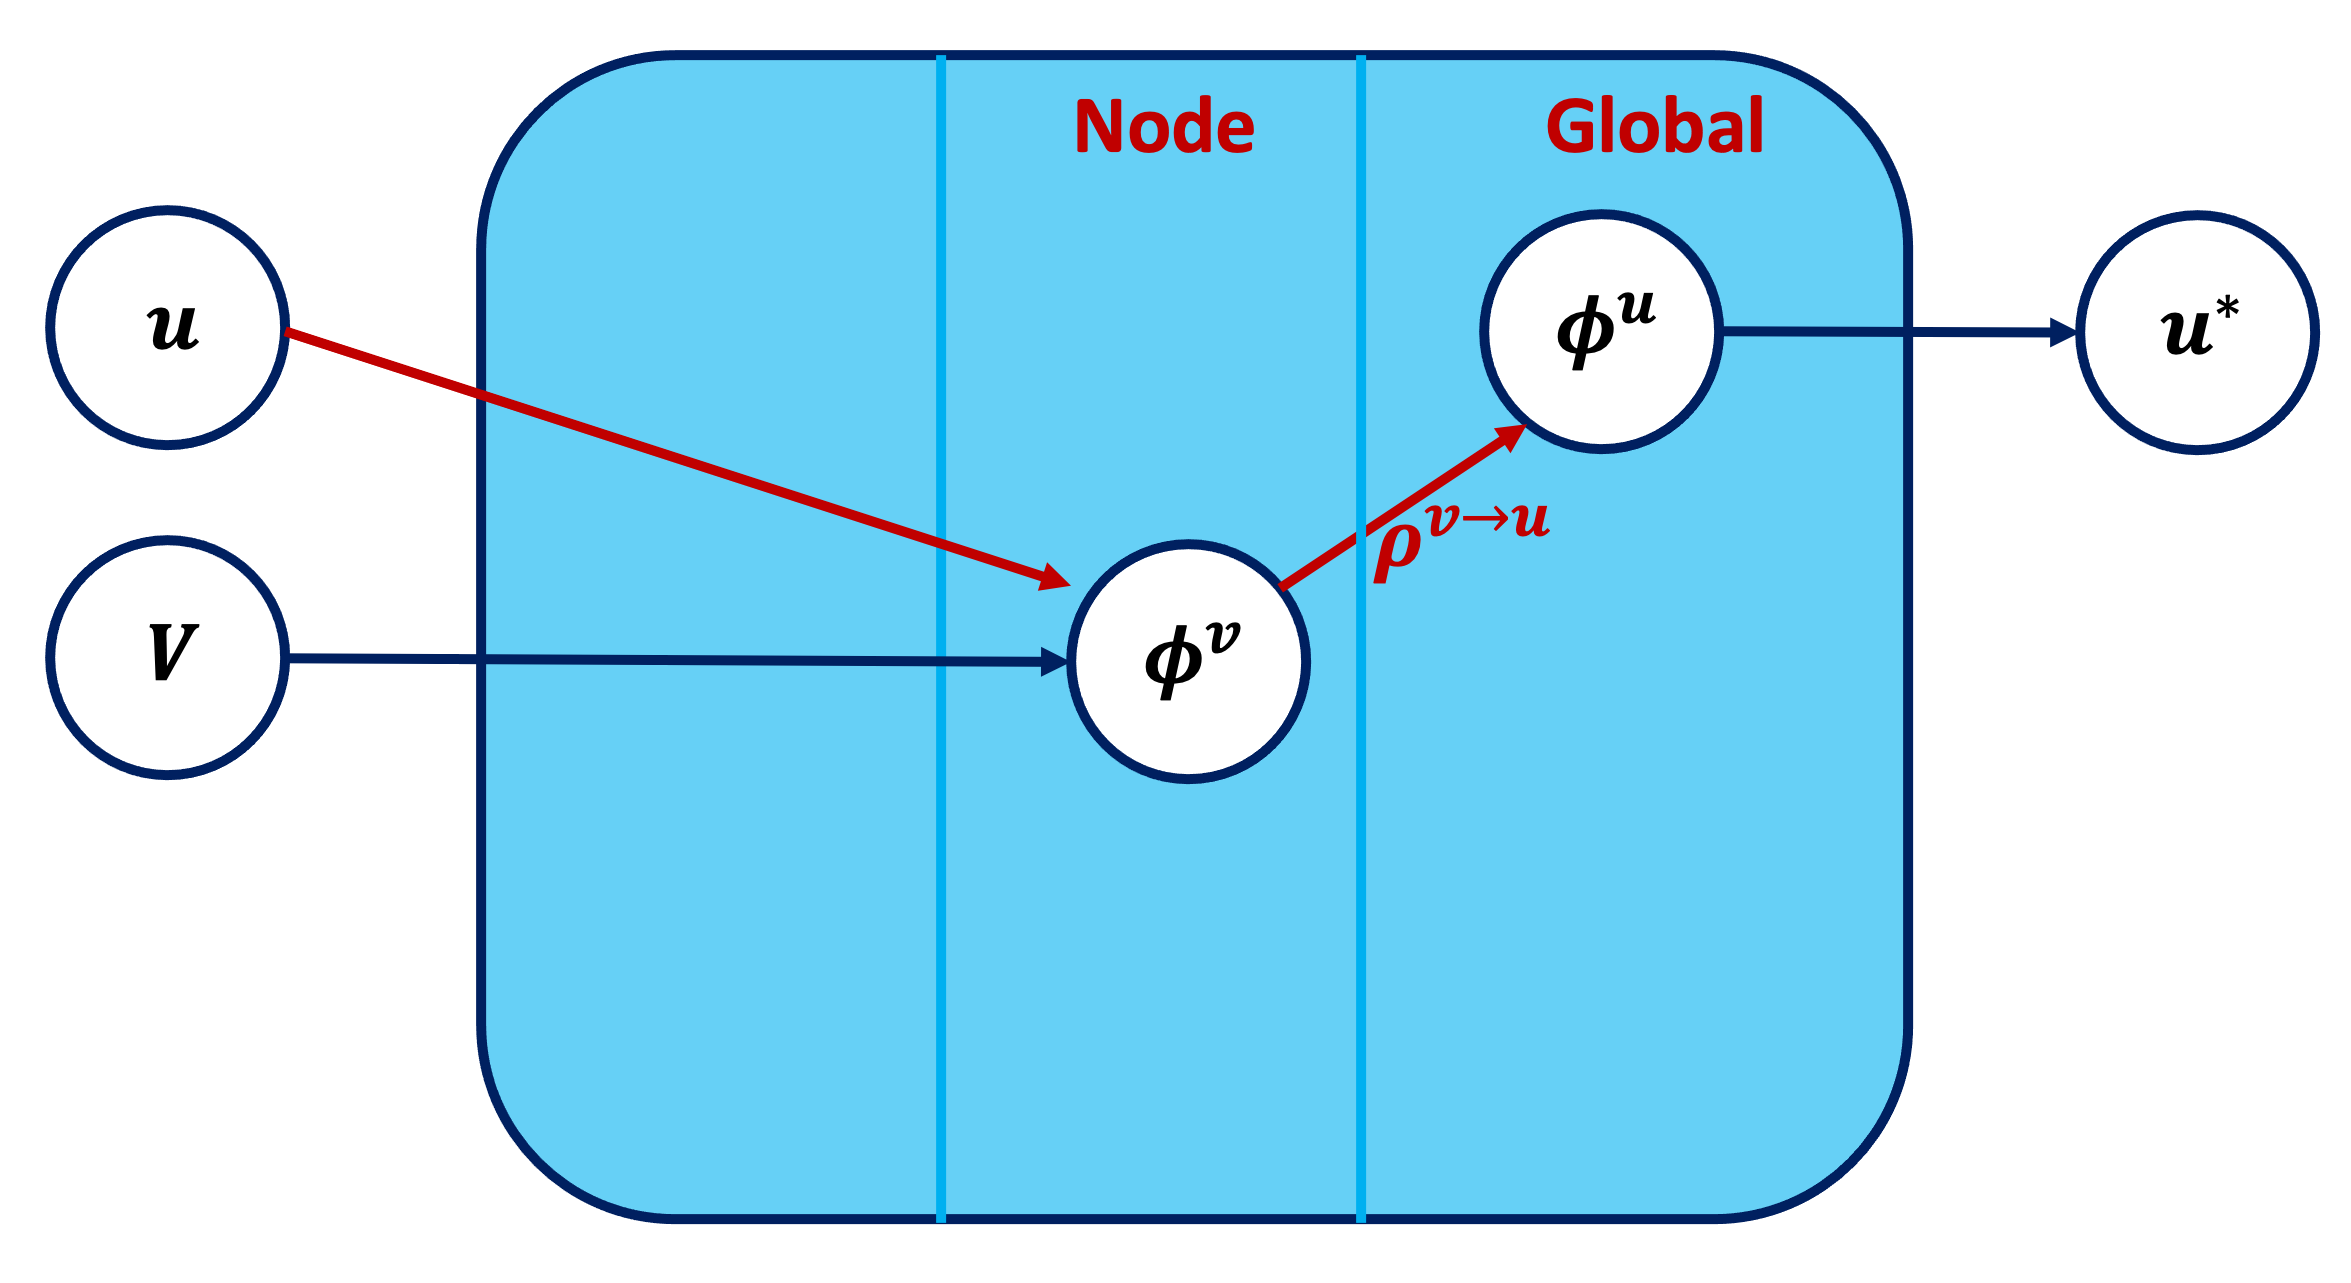
\includegraphics[scale=0.43]{Images/ML/deepSet.png}
        \caption{Deep Set.} 
        \label{fig:deepSetFig}
    \end{subfigure}
    \hfill
    \begin{subfigure}[b]{0.49\textwidth}
        \centering
        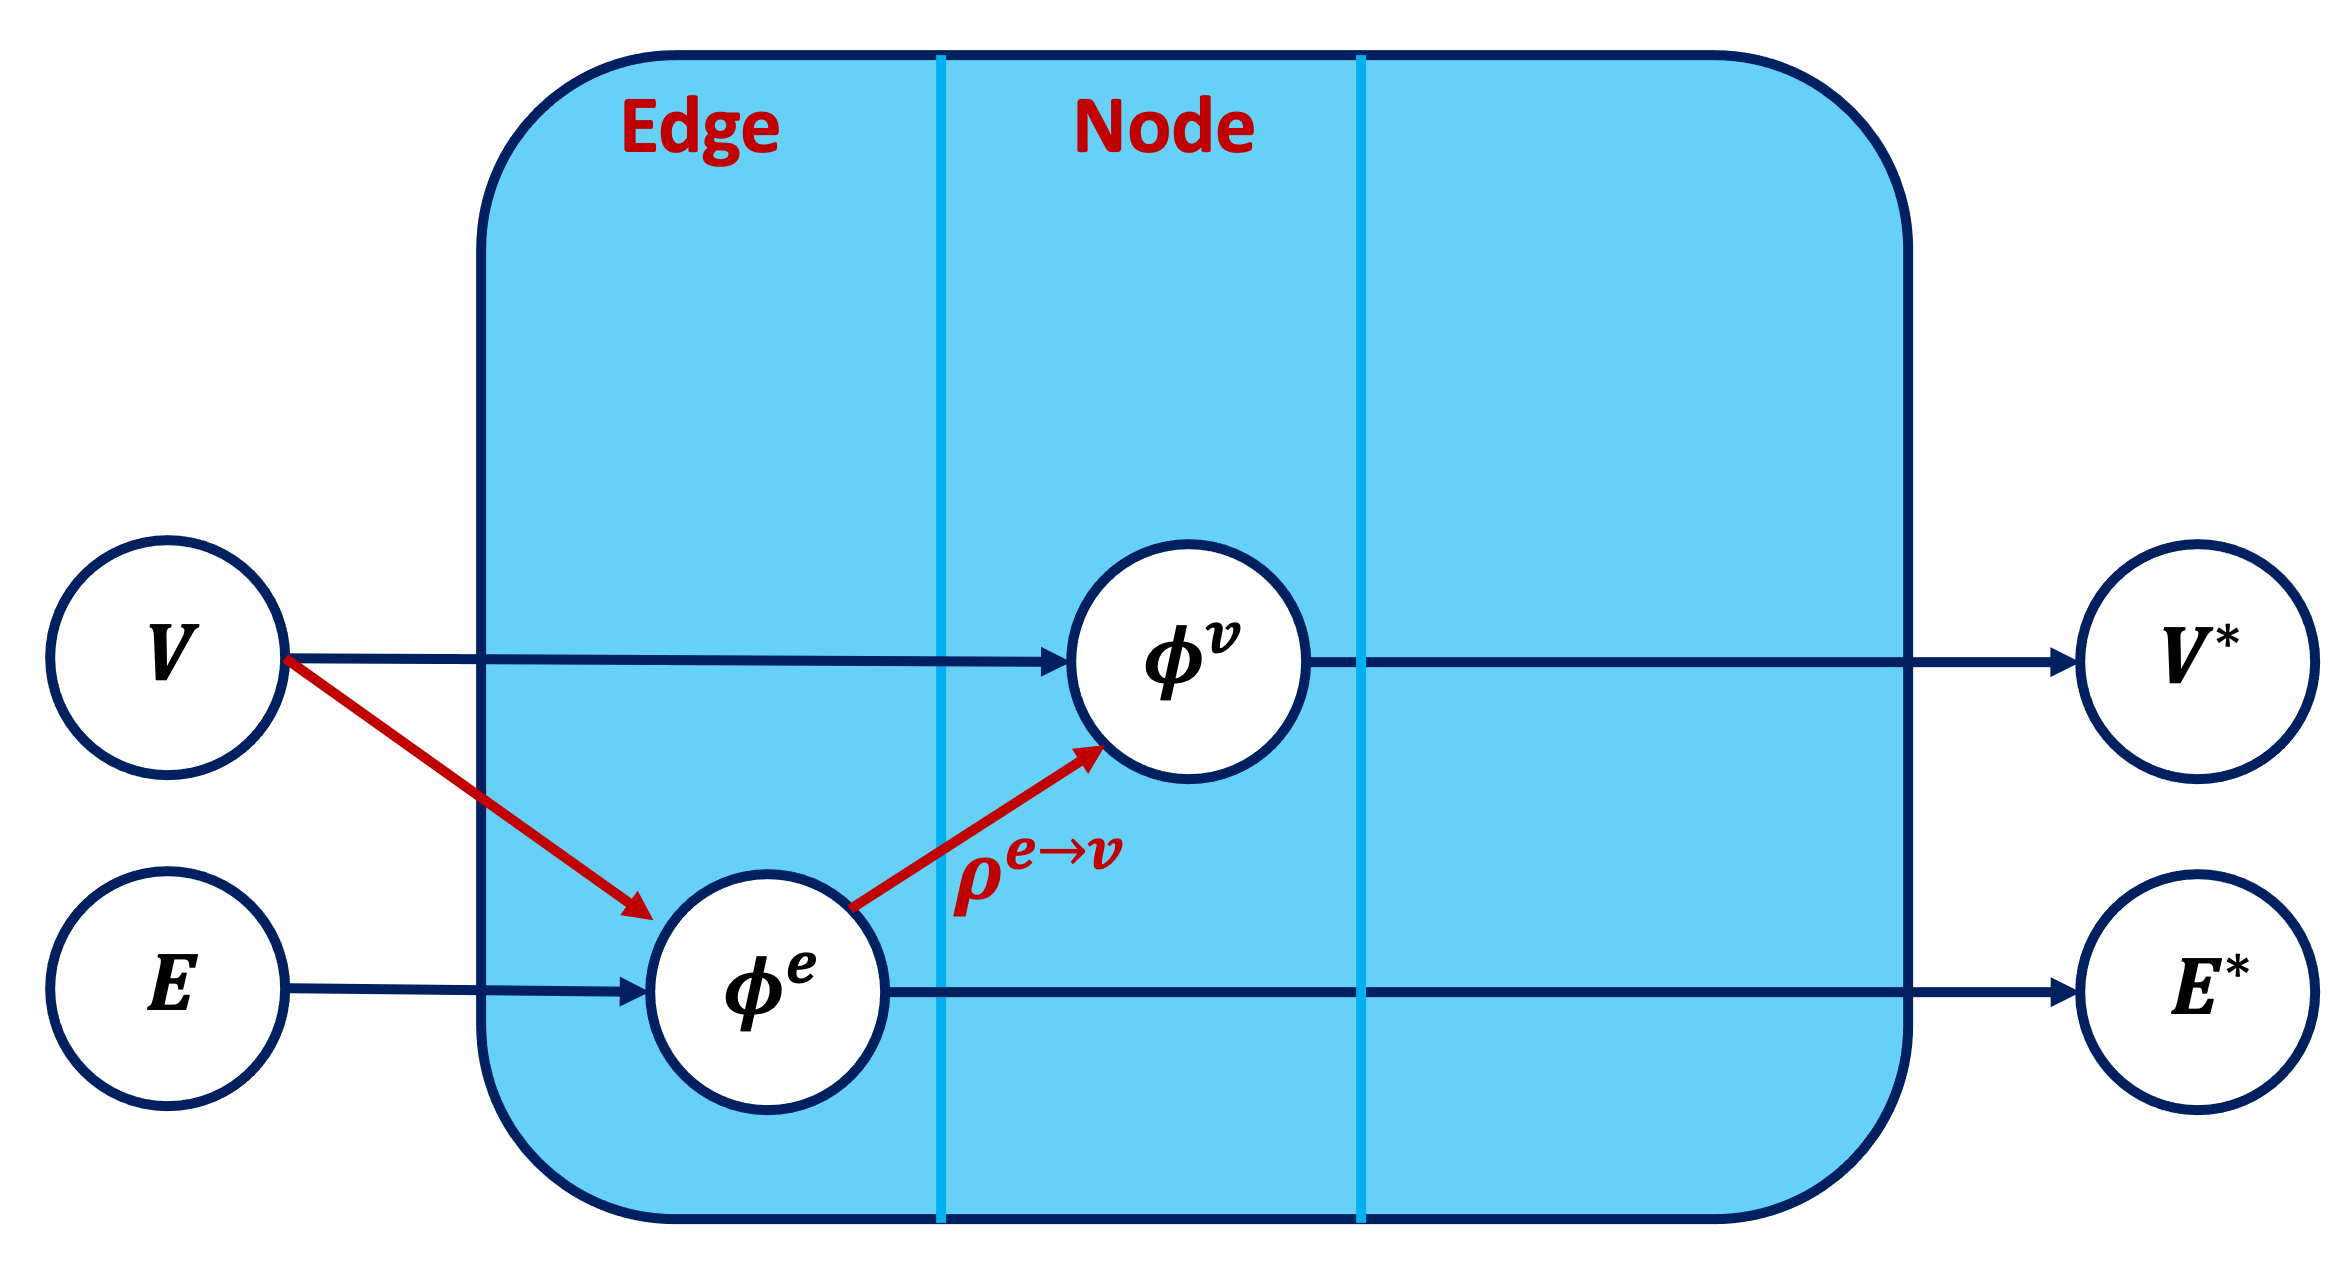
\includegraphics[scale=0.43]{Images/ML/nlnn.png}
        \caption{Non-local \gls{nn}.} 
        \label{fig:pullsFTAGnlnn}
    \end{subfigure}
    \caption{Different types of \gls{gnn} update rules, defining different \gls{gnn} architectures \cite{graphInductiveBias}.}
    \label{fig:diverseGNN}
\end{figure} 

A different approach introduced in \cite{nlnnPaper} defines the non-local neural network, unifying different types of \textit{attention}-based architecture. Attention is an essential feature of modern deep learning: it refers to a weighted version of the inputs, with weights standing for the degree of attention to be given to the different parts. Attention is not restricted to \gls{gnn} but is easily encapsulated in its formalism. As will be shown in the next section, the transformer is a special case of a non-local \gls{nn}. In this section, only the \gls{gat} is introduced for the sake of conciseness \cite{velickovic2018graph}. \glspl{gat} implement a learnable weighting of the neighbours of the node being updated. When updating node $v_i$, a score is computed for each of the connected neigbours $v_j$ of $v_i$ by a \gls{nn} mapping \[e(v_i, v_j) = \phi(v_i, v_j) = a^T \text{ leakyReLU}([W v_i, Wv_j]),\] where the nodes $v_i, v_j \in \mathbb{R}^d$ are connected and the operation implements an embedding of the two nodes to a dimension $d'$ with two learnable parameters: $a \in \mathbb{R}^{2d'}$ and $W \in \mathbb{R}^{d' \times d}$. The operator $[,]$ stands for matrix concatenation. These scores are then combined for each node $i$ over its neighbours $\{j\}$ to give $\alpha_{ij}$ attention scores \[ \alpha_{ij} = \text{softmax}_j (e(v_i, v_j)) = \frac{\exp(e(v_i, v_j))}{\sum_{j' \in \text{neighours of i}}e(v_i, v_{j'})}.\] The final step is to leverage these attention weights when updating each node $v_i$ as \[v^*_i = \sigma\left(\sum_{j} \alpha_{ij} W^v v_j \right),\] where the sum over $j$ is taken over neighbouring nodes of $i$, $\sigma$ is an activation function, and $W^v$ is another matrix of learnable parameters.

\paragraph{Pros:}
\begin{itemize}
    \item \textit{Modeling Graph Structure:} \glspl{gnn} naturally handle graph-structured data, making them well-suited for tasks involving abritrary relationships between entities.
    \item \textit{State-of-the-Art Performance:} \glspl{gnn} have achieved state-of-the-art results in various graph-related tasks.
\end{itemize}

\paragraph{Cons:}
\begin{itemize}
    \item \textit{Computational Complexity:} training \glspl{gnn} can be computationally expensive.
    \item \textit{Limited Global Context:} some \gls{gnn} architectures may struggle to capture long-range dependencies in graphs, limiting their ability to consider global context.
    \item \textit{Interpretability:} \glspl{gnn} are not directly interpretable.
\end{itemize}

\subsection{The Rise of the Transformers}\label{sec:transformer}
The transformer architecture, introduced in 2017 \cite{NIPS_transformerPaper}, has become a foundational and ubiquitous design across machine learning. It has significantly impacted the field, enabling the development of state-of-the-art models such as BERT \cite{devlin-etal-2019-bert} and GPT \cite{radford2018improving}. More recently, the transformer is also spearheading a revolution in computer vision tasks thanks to the generalisation of the architecture into the Vision Transformer (ViT) \cite{vitPaper}.\\

The transformer architecture is based on the mechanism of self-attention introduced in the previous section. It removes the sequential processing of \gls{rnn} by favouring a fully parallelisable approach, allowing for efficient computation on dedicated hardware. The key components in the transformer are the self-attention mechanism and position-wise feed-forward networks. Self-attention allows the model to weigh the importance of different words or tokens in a sequence for each token. This mechanism enables the model to capture long-range dependencies in the input data without the added complexity of \gls{lstm}. Strictly speaking, the input of a transformer is an unordered sequence that has no strict order. For \gls{nlp}, the ordering is built into the model with position-wise embedding, giving the model a handle to determine the index of the token in the sequence. In computer vision, the vision transformer first splits the input image $x$ into patches of fixed size, flattens them into a vector, and maps them with a learnable positional embedding before processing them as a classical transformer.

\begin{figure}[h!]
    \center
    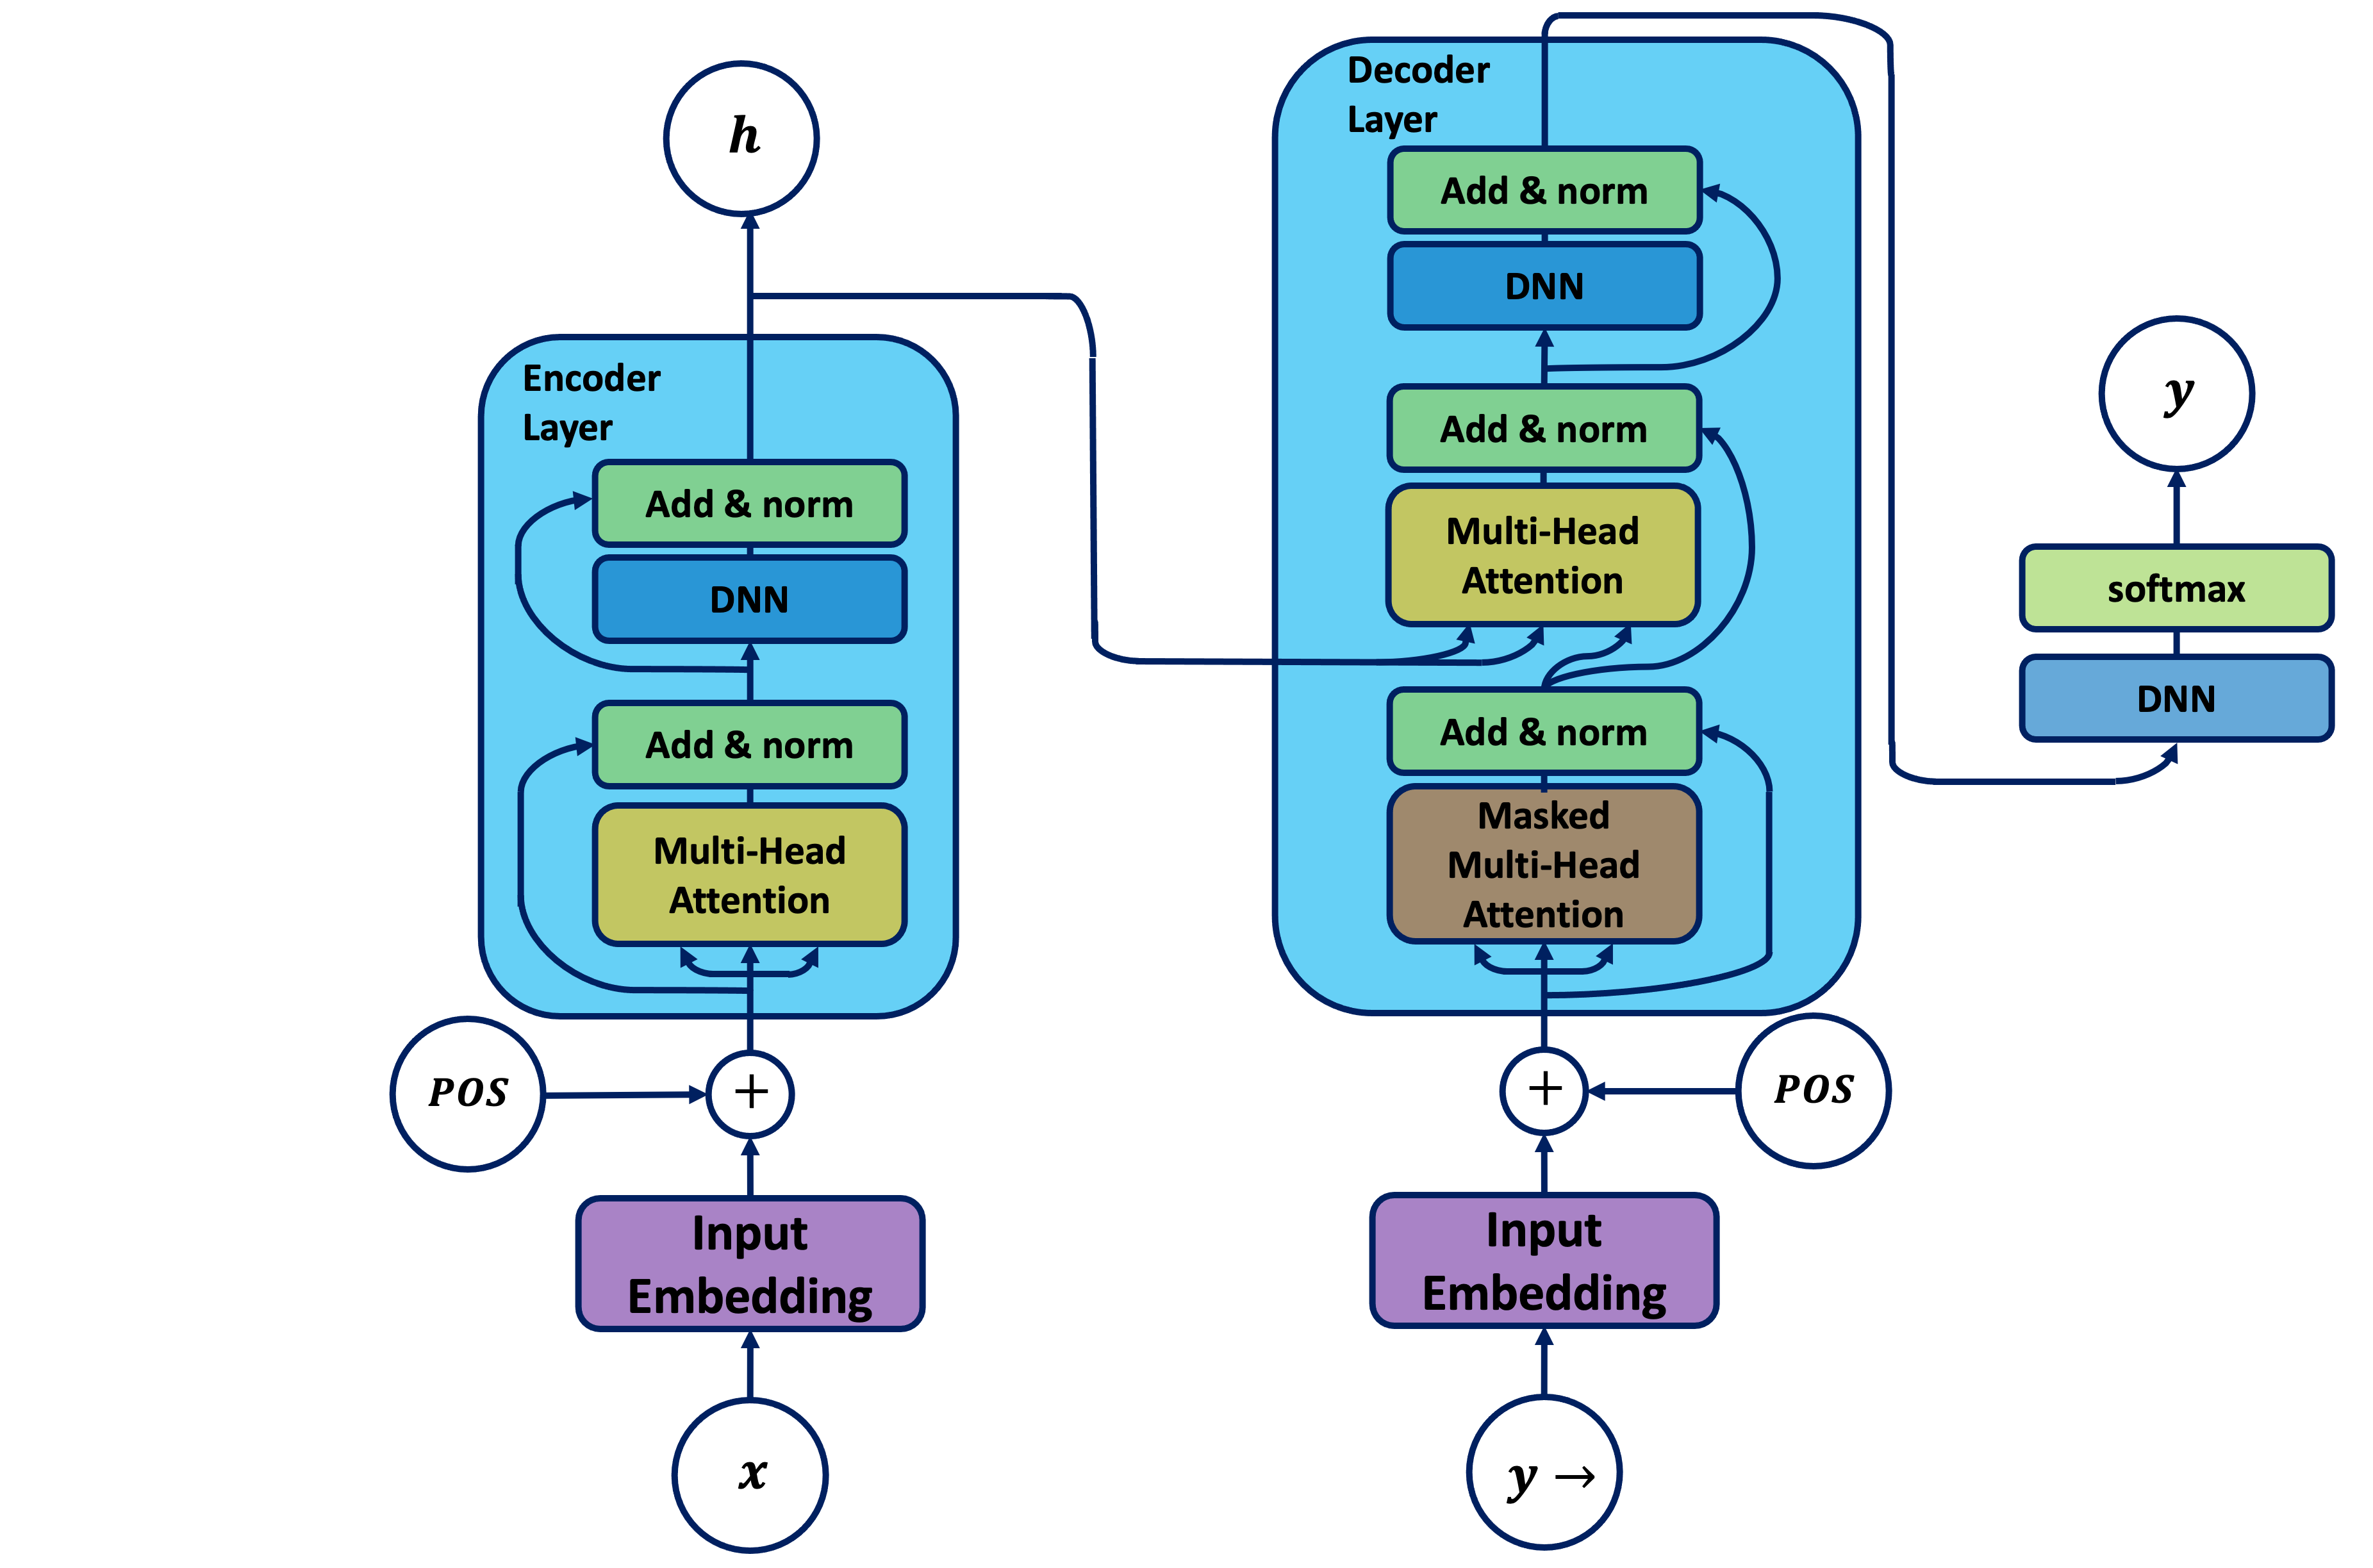
\includegraphics[width=\textwidth]{Images/ML/transformer.png}
    \caption{The full transformer architecture, combining an encoder and a decoder each made of an arbitrary number of layers. The input $x$ is first embedded with a dedicated mapping which can, when order matters, be supplemented with positional embedding. The encoder generates an internal representation $h$ that is passed to the decoder. This component, depicted on the right, produces the next output using the internal representation $y$ and the output shifted to the right - to force output tokens to only access prior information.} 
    \label{fig:tranfoArchi}
\end{figure}

The general transformer architecture, presented in Figure~\ref{fig:tranfoArchi}, consists of an encoder and a decoder. The decoder works in an autoregressive way, combining the current outputs $y_{t<T}$ with an internal representation $h$ built by the encoder to generate the next output tokens $y_{T}$. Both the encoder and the decoder are composed of multiple layers, each containing a multi-head self-attention mechanism and position-wise feed-forward networks (\gls{dnn}). The decoder is further endowed with a masked attention layer, for the output to compute self-attention with information accessible before the token's position. The attention mechanism allows the model to focus on different parts of the input sequence, while the feed-forward networks provide additional non-linear transformations. Residual connexions are added to let the gradients propagate efficiently in-depth and layer normalisation is used after each block to avoid vanishing or exploding gradients and improve training speed \cite{ba2016layer}. This type of normalisation scales each activation (each neuron) by subtracting the empirical mean and dividing by the standard deviation per data point. \\

The attention mechanism maps the queries and a set of key-value pairs to an output as defined in Equation \ref{eq:scdotatt} and schematised in Figure~\ref{fig:scaledDotAtt}, with query $Q \in \mathbb{R}^{d_k \times d_q}$, key $K \in \mathbb{R}^{d_k \times d_v}$, and value $V \in \mathbb{R}^{d_v}$ and the output is a vector $\mathbb{R}^{d_q \times d_v}$ of values reweighted by the attention scores. This combines $d_q$ different queries of the $d_k$ keys mapping to $d_v$ values. Therefore, Equation \ref{eq:scdotatt} implements for each query a weighted sum of the values, based on a compatibility function established by comparing the queries and keys:
\begin{equation}\label{eq:scdotatt}
    \text{Attention}(Q, K, V) = \text{softmax}\left( \frac{Q^T \, K}{\sqrt{d_k}}\right) V,
\end{equation} 
where the scaling by $\sqrt{d_k}$ is implemented to reduce the magnitude of the dot product $Q^T K$ and avoid landing in regions of saturation of the subsequent softmax, which is applied per row of the formed attention matrix. This scaled dot-product attention mechanism leverages the extensive research into numerical optimisation of matrix multiplications, making this operation less time and memory-consuming than using a \gls{dnn} mapping to compute the attention - a technique referred to as \textit{additive attention} \cite{Bahdanau2014NeuralMT}. As shown in Figure~\ref{fig:mulitheadAtt}, multi-head attention runs this dot-product attention in parallel for $h$ different heads, each head $h_i$ ($i = 1, ..., h$) implementing a separate learnable projection from the input $Q$, $K$, $V$ with linear transformations of respective weights $W_i^Q \in \mathbb{R}^{d \times d_k}$, $W_i^K \in \mathbb{R}^{d \times d_k}$, and $W_i^Q \in \mathbb{R}^{d \times d_v}$, where $N$ is the length of the sequence, $d$ is the model dimension and $h$ the number of heads: \[Q_i = Q W_i^Q, \quad K_i = K W_i^K, \quad V_i = V W_i^V,\] \[H_i = \text{Attention}(QW_i^Q, KW_i^K, VW_i^V).\] The multi-head module then concatenates the $h$ different heads $H_i$ outputs and applies another linear tranformation of parameters $W^O \in \mathbb{R}^{hd_v \times d}$ \[\text{Multi-Head Attention}(Q, K, V) = \left[H_1, ..., H_h\right]W^o .\] In multi-head attention, there are therefore 3 different learnable projections $W_i^Q$, $W_i^K$, and $W_i^V$ per head and a single global projection $W^O$ for the output of the cell. Self-attention is a special case in which the input of the cell is not a tuple $(Q, K, V)$ of distinctive vectors but a single input $x \in \mathbb{R}^{N \times d_v}$ that is mapped out to the tuple with the learnable projections: \[Q = xW_i^Q, \quad K = xW_i^K, \quad V = xW_i^V.\]

\begin{figure}[h!]
    \centering
    \begin{subfigure}[b]{0.49\textwidth}
        \centering
        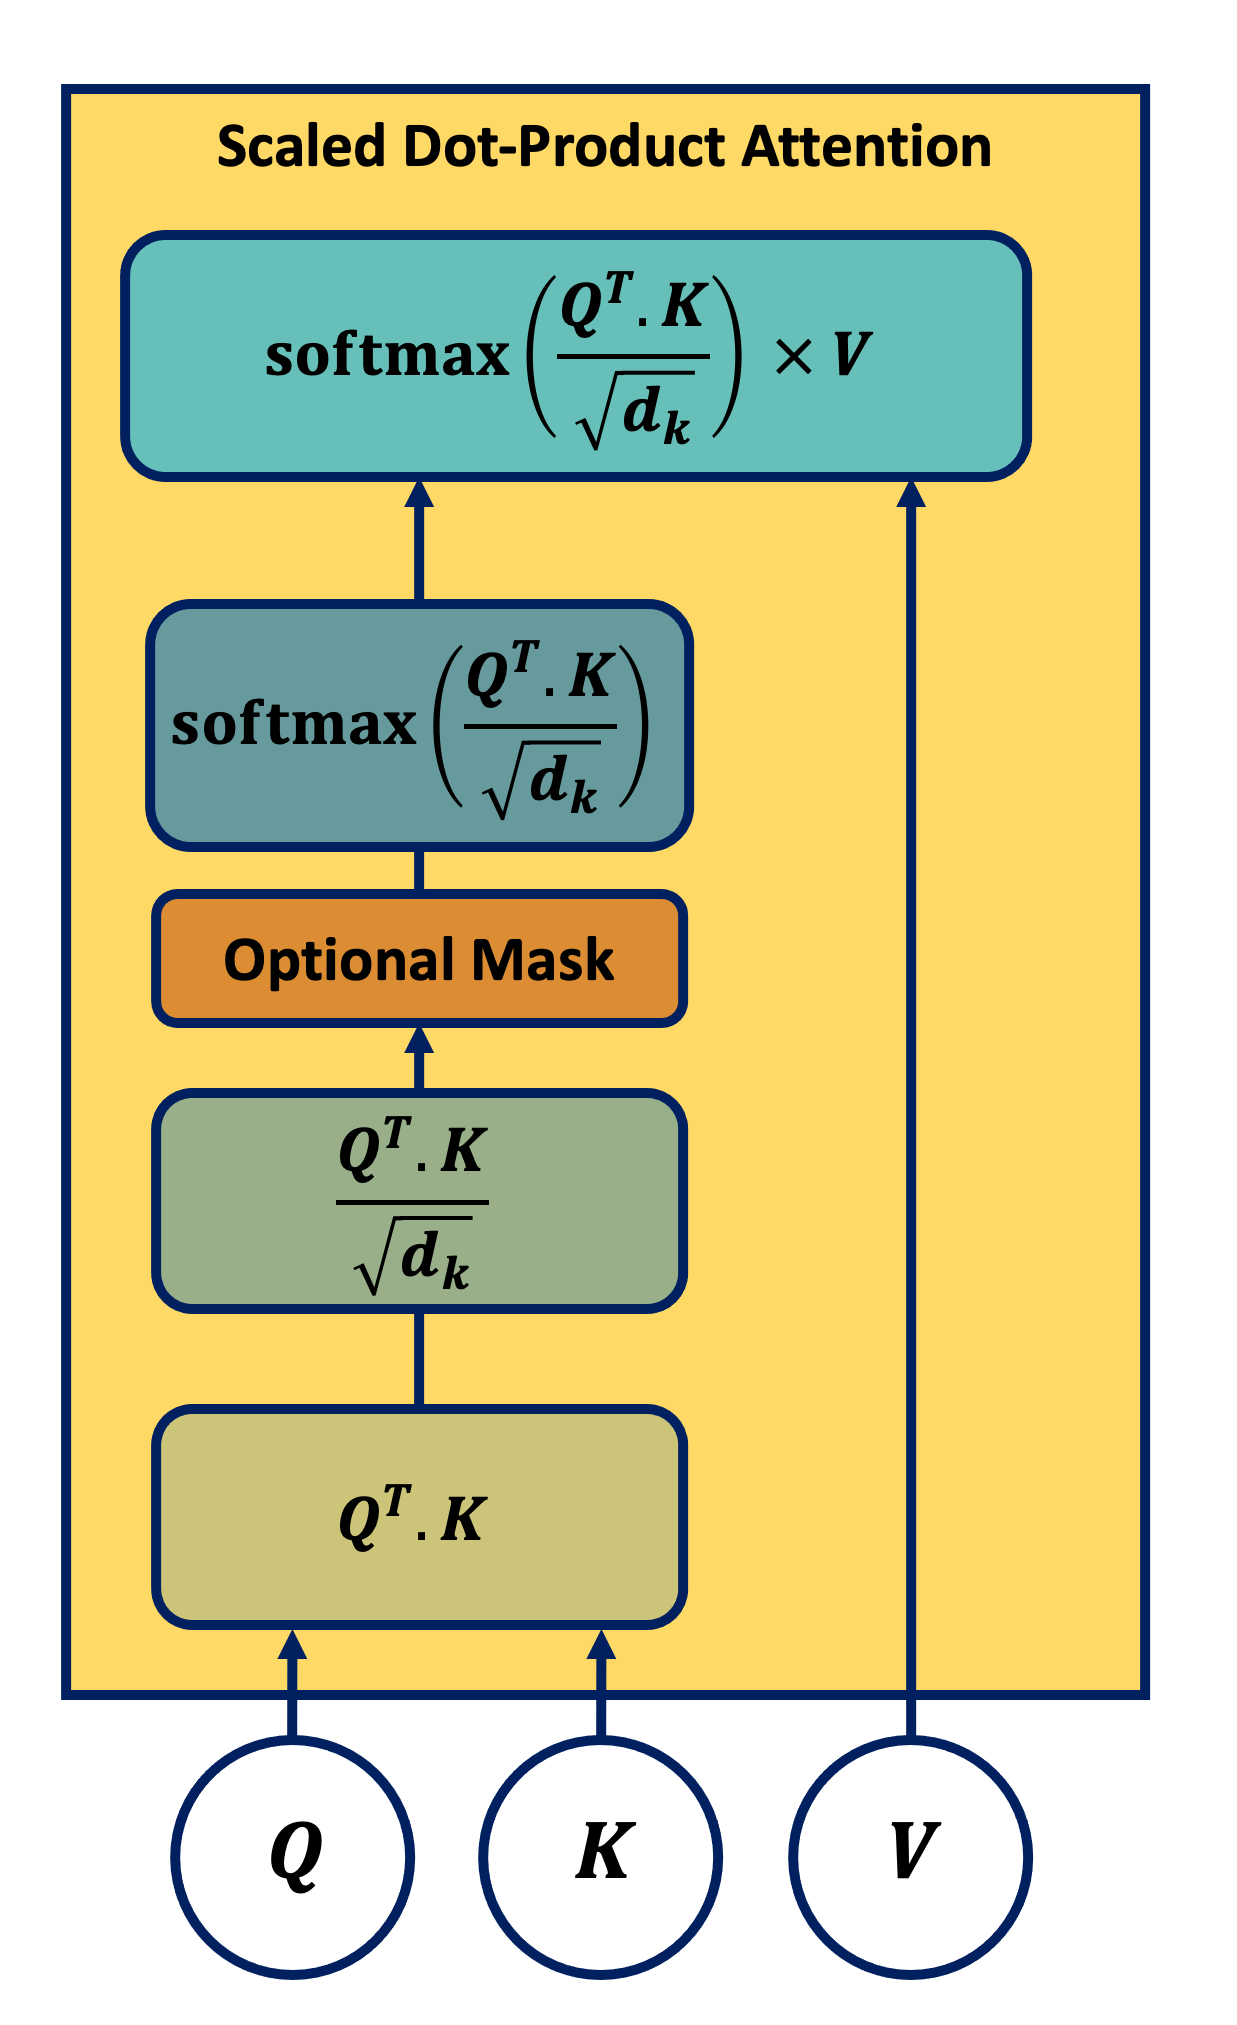
\includegraphics[scale=0.65]{Images/ML/scaledDotAtt.png}
        \caption{Scaled dot-product attention with optional masking.} 
        \label{fig:scaledDotAtt}
    \end{subfigure}
    \hfill
    \begin{subfigure}[b]{0.5\textwidth}
        \centering
        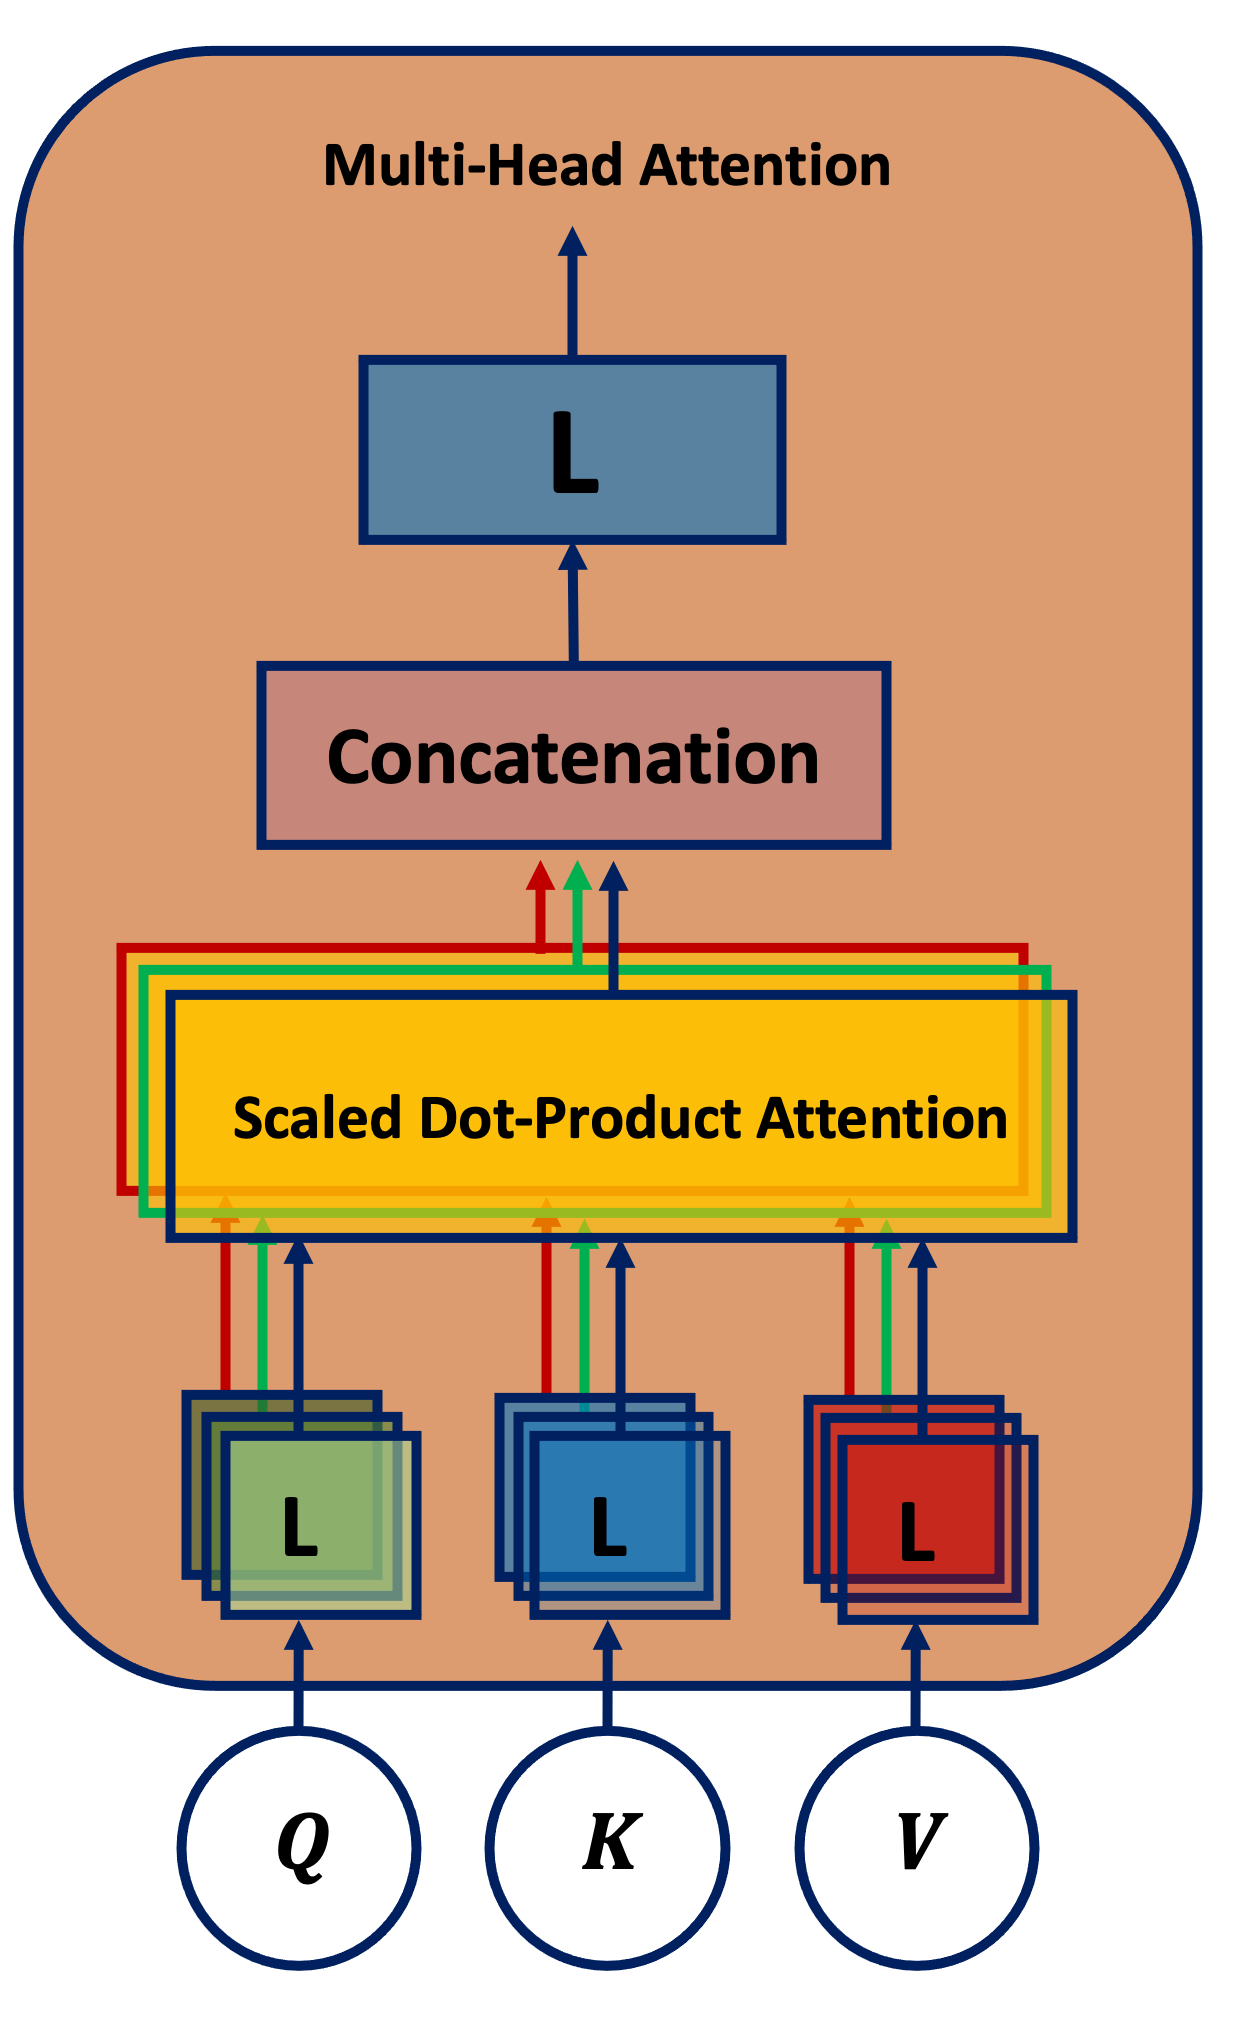
\includegraphics[scale=0.65]{Images/ML/multiHeadAtt.png}
        \caption{Multi-head attention module, where $L$ stands for a linear transformation of the input.} 
        \label{fig:mulitheadAtt}
    \end{subfigure}
    \caption{Multi-head attention mechanism in a transformer. The core operation is an optionally masked scaled dot-product of the queries $Q$, keys $K$, and values $V$. A head consists of three (optionally different) linear projections of the tuple $(Q, K, V)$, each leading to a separate scaled dot-product. The multi-head modules then concatenate all the different head results and finish with another linear transformation.}
    \label{fig:transAtt}
\end{figure} 

\paragraph{Pros:}
\begin{itemize}
    \item \textit{Versatility:} the transformer architecture has been successfully applied to various \gls{nlp} and computer vision tasks.
    \item \textit{Parallelisation:} the architecture is efficiently parallelised, speeding up the computations.
    \item \textit{Capturing Dependencies:} the self-attention mechanism enables the model to capture complex long-range dependencies.
    \item \textit{Stability:} transformers benefit from inbuilt regularisation effects due to residual connexions and normalisation layers. Models based on this structure can therefore simply scale in complexity and resist well to overtraining.
\end{itemize}

\paragraph{Cons:}
\begin{itemize}
    \item \textit{Computational Complexity:} large transformer are computationally expensive to train.
    \item \textit{Interpretability:} the attention mechanism is challenging to interpret.
    \item \textit{Data Dependency:} transformer models require large amounts of data for effective training, limiting their application in domains with limited statistics.
\end{itemize}

\section{Training and Optimising Deep Learning Models}
Training and optimising neural network involve a combination of selecting appropriate architectures, fine-tuning the hyperparameters that are not learnt by backpropagation, and employing acceleration techniques to improve efficiency and convergence. In this section, key aspects of the training process are explored.

\subsection{Training Algorithms}
When optimising the learnable parameters of a model, different training algorithms can be deployed to update the weights. All strategies are refinements of the gradient descent rule of Equation \ref{eq:gradientdescent}, and each method has different advantages. The two main approaches are: 
\begin{itemize}[leftmargin=*]
    \item \gls{sgd}: instead of deriving the gradients on the whole dataset (full-batch), the expectated gradient over a random sub-batch of $b$ elements is taken, hence the stochastic behaviour \[ \nabla w = \frac{1}{b} \sum_{s=1}^b \nabla w_s,\] with $\nabla w_s$ the gradient of the parameter $w$ computed for a single data point. A common observation is that for sub-batches - from now on referred to as just \textit{batches} - of sufficient size $b$, the statistical estimator of the gradient based on the batch is unbiased. This greatly reduces the time needed to compute the gradient and naturally splits the loop over the dataset into different iterations called \textit{steps}, at which a batch is passed through the network, a beneficial feature in the case of large datasets that would not fit in memory. This has also an effect on the regularisation of the model, as each per-batch gradient has a larger variance than a full-batch, making it harder for the model to overtrain but slowing the convergence to an optimum. 
    \item Adam is an algorithm published in 2014 leveraging an adaptive moment estimation approach as well as batch processing \cite{adamPaper}. The moment in this sense is analogous to the physical moment and encapsulates the dynamic of the optimisation as driven by gradient descent. The fundamental idea is that larger gradients indicate a steeper slope that can be quickly traversed so that any slowing-down due to a changing curvature of the objective function landscape can be mitigated from to the inertia of the previous gradients. This behaviour is implemented as an exponentially decaying moving average: the moment $m^t_w$ of weight $w$ at step $t$ is updated with a gradient forgetting factor $\beta_1 \in [0, 1[$ such that \[ m_t \leftarrow \beta_1 m^{t-1}_w + (1 - \beta_1) \nabla w_s^t,\] where the previous contribution is successively multiplied by $\beta_1$, reducing the importance of earlier gradients progressively. Additionally, another element is taken into account in the gradient descent rule: the second moment $(\nabla w_s^t)^2$. This tracks the magnitude of the gradient and, by multiplying the gradient update by a term inversely proportional to the second moment, accelerates the gradient updates in flatter regions of the objective landscape giving small gradient magnitudes with the term \[ v_t \leftarrow \beta_2 v^{t-1}_w + (1 - \beta_2) (\nabla w_s^t)^2,\] where a second-moment forgetting factor $\beta_2 \in [0, 1[$ is introduced. To avoid biasing the gradient update, both the momentum (first moment) and the second moment are corrected with \[\hat{m}^t_w \leftarrow \frac{m^t_w}{1 - \beta_1} \quad \text{ and } \quad  \hat{v}^t_w \leftarrow \frac{v^t_w}{1 - \beta_2}.\] The two contributions are then combined into a single gradient descent step as
    \begin{equation}\label{eq:adam}
        w^{t} \leftarrow w^{t-1} - lr \times \frac{\hat{m}^t_w}{\sqrt{\hat{v}^t_w} + \epsilon},
    \end{equation}
    where a very small $\epsilon$ is added for numerical stability.
\end{itemize}

A key hyperparameter in any gradient descent-based algorithm is the learning rate $lr$. There is no evident choice for this parameter and suitable values have to be derived on a case-by-case approach. A useful technique to let the training process converge to a good minimum of the loss function and avoid unsuitable local minima is to adopt a \textit{learning rate schedule}, modifying the parameter throughout training to resolve different parts of the loss function landscape. Initially, a relatively large $lr$ allows the model to quickly update its weights in the direction of the minimum. If the rate is kept too high, the weights will not be able to approach the minimum and will overshoot or ``bounce' around the optimal set. To avoid this, the scheduler reduces the learning rate so that smaller steps can be taken later to approach the chosen optimum. At the beginning, the rate is typically not set to its maximum to move the gradient updates to a valley of interest. An equivalent choice is to modify the batch size while keeping the $lr$ fixed \cite{smith2017decay}. This has also a regularising effect on the gradient: small batch sizes capture large variances and let the optimisation make drastic changes of orientation in the optimising function landscape, thereby avoiding unsatisfactory local minima. Larger batch sizes stabilise the direction of descent, thereby offering a lower variance but potentially biased estimates towards a minimum. Combining these two characteristics at different epochs of the training is an effective way to improve the training performance. Some methods, such as Adam, have other specific hyperparameters that should be optimised.

\subsection{Regularisation}
Regularisation techniques are applied in the architecture and training procedure to prevent overfitting. Common methods include \textit{dropout}, which randomly drops connexions or neurons during training and L2 (L1) regularisations that penalises large weights proportionally to a penalisation parameter $\lambda$ times the sum of the squared (absolute value) of the weights. Both $p$ and $\lambda$ require careful optimisation as regularising the model can introduce bias and hit the overall performance. Additionally, batch normalisation is a technique that normalises the inputs of a layer over the batch, reducing internal covariate shifts. It helps stabilise and accelerate the training process. This is distinct from the layer normalisation used in the transformer architecture, as the normalisation is carried over the batch samples rather than the activations. 

\subsection{Architecture \& Hyperparameters Optimisation}
Several characteristics of the network need to be optimised: 
\begin{itemize}[leftmargin=*]
    \item \textit{Architecture Selection:} choosing the right architecture is crucial for the success of a \gls{nn}. Factors to consider include the complexity of the task, the nature of the data, and the desired trade-off between model complexity and interpretability. Limits in computing power should be factored in. Elements of the architecture include the type of \gls{ml} chosen (\gls{bdt}, \gls{dnn}, transformer, ...), the choice of activation functions (\gls{relu}, tanh, ...), and the number of layers, nodes, and connexions between the units.
    \item \textit{Hyperparameter Tuning:} optimising the hyperparameters - parameters that are not optimised through backpropagation of the loss - is essential for achieving the best possible performance. Key hyperparameters include optimiser-related parameters such as the learning rate, the batchsize, regularisation parameters, and initialisation of the weights and biases.
\end{itemize}
The optimisation process for both hyperparameter tuning and architecture selection is expensive: the model must be trained with different combinations of hyperparameters or architecture to evaluate their respective performance and uncover the best-performing options. Techniques such as grid search, random search, and Bayesian optimisation can be employed to efficiently explore the hyperparameter space. Architecture search is usually performed by trial and error, with the \gls{ml} literature offering little insight into what models might best perform in specific situations. 

\subsection{Acceleration Techniques}
Training an \gls{ml} model is often a computationally demanding task that can be carried out more effectively on specifically designed hardware and with some tricks in the process. 
\begin{itemize}[leftmargin=*]
    \item \textit{Parallel Dataloading:} can significantly speed up the training process. Instead of preparing a single batch, multiple batches can be loaded by different processing units in parallel to avoid this bottleneck. 
    \item \textit{Early Stopping:} prevents overfitting and save computation time by interrupting the training when the performance saturates.
    \item  \textit{Hardware Accelerators:} specialised hardware accelerators can accelerate the training. The \glsfirst{gpu} is specially designed to perform matrix operations in parallel, and therefore well suited for \gls{ml}. Utilising \glspl{gpu} for training and inference can give substantial speedups compared to \gls{cpu}-based computing. 
    \item \textit{Transfer Learning:} leverages pre-trained models on large datasets and applies them to a new task. The idea is that there are some fundamental similarities between the new task and the task used to pre-train the foundational model giving the latter a headstart. Fine-tuning these models on specific tasks or connecting additional modules can significantly reduce the required training time and data compared to training from scratch. This approach is becoming increasingly fashionable, as larger \textit{foundational} models trained on multiple tasks with huge datasets can then be applied to a specific task, with the pre-trained weights either kept fixed or modified for the new task. Such large foundational models are already available in \gls{nlp} (e.g., the 7 billion parameters transformer Mistral 7B \cite{jiang2023mistral}) and computer vision (e.g., the 500 million parameters Florence-2 \cite{xiao2023florence2}).
\end{itemize}
Training and optimising deep learning models involve a combination of careful architectural choices, hyperparameter tuning, and the use of acceleration techniques. Selecting the most appropriate techniques is a task-specific challenge that depends on available resources and trade-offs between training time, model performance, and interpretability.
